%==============================================================================
%  Handbook of Triaxial Hopkinson Pressure Bar Testing and Experiments
%
%  Author : Qianbing Zhang
%  Affil. : Department of Civil and Environmental Engineering,
%           Monash University, Wellington Road, Clayton, VIC 3800, Australia
%  Contact: qianbing.zhang@monash.edu
%
%  Compiles with pdfLaTeX (TeX Live 2022+).
%==============================================================================

\documentclass[11pt,a4paper,openany]{book}
\raggedbottom

% ---------------- Packages -----------------------------------------------------
\usepackage[utf8]{inputenc}
\usepackage[T1]{fontenc}
\usepackage{lmodern}
\usepackage{microtype}
\usepackage[margin=2.5cm,headheight=14pt]{geometry}
\usepackage{amsmath,amssymb,amsfonts,amsthm}
\usepackage{mathtools}
\usepackage{bm}
\usepackage{empheq}
\usepackage{siunitx}
% siunitx v3 removed \SI and \SIrange; v2 provided them. Compatibility shim:
\providecommand{\SI}[2]{\qty{#1}{#2}}
\providecommand{\SIrange}[3]{\qtyrange{#1}{#2}{#3}}
\usepackage{graphicx}
\usepackage{xcolor}
\usepackage{tcolorbox}
\IfFileExists{pdfcol.sty}{%
  \tcbuselibrary{breakable}%
  \newcommand{\tcbmaybeBreakable}{breakable}%
}{%
  \newcommand{\tcbmaybeBreakable}{}%
}
\usepackage{booktabs}
\usepackage{array}
\usepackage{longtable}
\usepackage{multicol}
\usepackage{enumitem}
\usepackage{titlesec}
\usepackage{fancyhdr}
\usepackage{tikz}
\usetikzlibrary{arrows.meta,positioning,calc,decorations.pathreplacing,patterns}
\usepackage[backend=biber,style=numeric,sorting=none,maxbibnames=99]{biblatex}
\usepackage{hyperref}

% ---------------- Colours ------------------------------------------------------
\definecolor{deepblue}{RGB}{31,56,100}
\definecolor{midblue}{RGB}{46,117,182}
\definecolor{accentpink}{RGB}{170,40,90}
\definecolor{accentcyan}{RGB}{0,140,170}
\definecolor{warnorange}{RGB}{210,110,20}
\definecolor{dangerred}{RGB}{180,40,60}
\definecolor{boxgrey}{RGB}{245,247,250}
\definecolor{rulegrey}{RGB}{210,215,225}
\setlength{\parskip}{6pt plus 2pt minus 1pt}
% ---------------- Hyperref -----------------------------------------------------
\hypersetup{
  colorlinks=true,
  linkcolor=deepblue,
  citecolor=midblue,
  urlcolor=midblue,
  pdftitle={Handbook of Triaxial Hopkinson Pressure Bar Testing and Experiments},
  pdfauthor={Qianbing Zhang},
  pdfsubject={Triaxial split Hopkinson pressure bar testing of geomaterials},
  pdfkeywords={SHPB, Tri-HB, dynamic testing, stress wave, damage mechanics, DEM}
}

% ---------------- Title formatting --------------------------------------------
\titleformat{\chapter}[display]
  {\normalfont\huge\bfseries\color{deepblue}}
  {\filright\Large\chaptertitlename\ \thechapter}
  {1ex}
  {\vspace{0.6ex}{\color{rulegrey}\titlerule[0.8pt]}\vspace{1ex}\Huge\filright}
\titlespacing*{\chapter}{0pt}{-20pt}{30pt}

\titleformat{\section}
  {\Large\bfseries\color{deepblue}}
  {\thesection}{0.6em}{}
  [\vspace{2pt}{\color{rulegrey}\hrule height 0.4pt}]
\titleformat{\subsection}
  {\large\bfseries\color{midblue}}
  {\thesubsection}{0.6em}{}
\titleformat{\subsubsection}
  {\normalsize\bfseries\color{midblue}}
  {\thesubsubsection}{0.6em}{}

% ---------------- Page style ---------------------------------------------------
\pagestyle{fancy}
\fancyhf{}
\fancyhead[LE,RO]{\small\color{deepblue}\thepage}
\fancyhead[LO]{\small\color{deepblue}\nouppercase{\rightmark}}
\fancyhead[RE]{\small\color{deepblue}\nouppercase{\leftmark}}
\renewcommand{\headrulewidth}{0.4pt}
\renewcommand{\headrule}{\color{rulegrey}\hrule height 0.4pt}

\fancypagestyle{plain}{%
  \fancyhf{}%
  \fancyfoot[C]{\small\thepage}%
  \renewcommand{\headrulewidth}{0pt}%
}

% ---------------- Custom boxes -------------------------------------------------
\newtcolorbox{conceptbox}[1][]{
  colback=boxgrey, colframe=midblue,
  boxrule=0.6pt, arc=2pt,
  fonttitle=\bfseries\color{white},
  coltitle=white, colbacktitle=midblue,
  title={#1}, \tcbmaybeBreakable,
  left=8pt, right=8pt, top=6pt, bottom=6pt
}
\newtcolorbox{stepbox}[1][]{
  colback=white, colframe=accentcyan,
  boxrule=0.8pt, arc=1pt,
  fonttitle=\bfseries\color{white},
  coltitle=white, colbacktitle=accentcyan,
  title={#1}, \tcbmaybeBreakable,
  left=8pt, right=8pt, top=6pt, bottom=6pt
}
\newtcolorbox{warningbox}[1][]{
  colback=boxgrey, colframe=warnorange,
  boxrule=0.8pt, arc=1pt,
  fonttitle=\bfseries\color{white},
  coltitle=white, colbacktitle=warnorange,
  title={#1}, \tcbmaybeBreakable,
  left=8pt, right=8pt, top=6pt, bottom=6pt
}
\newtcolorbox{newfeature}[1][]{
  colback=boxgrey, colframe=accentpink,
  boxrule=0.8pt, arc=1pt,
  fonttitle=\bfseries\color{white},
  coltitle=white, colbacktitle=accentpink,
  title={#1}, \tcbmaybeBreakable,
  left=8pt, right=8pt, top=6pt, bottom=6pt
}

% ---------------- Theorems / definitions ---------------------------------------
\newtheoremstyle{handbook}{1em}{1em}{}{}{\bfseries\color{deepblue}}{.}{0.5em}{}
\theoremstyle{handbook}
\newtheorem{definition}{Definition}[chapter]
\newtheorem{remark}{Remark}[chapter]

% ---------------- Maths shortcuts ----------------------------------------------
\newcommand{\sig}{\sigma}
\newcommand{\eps}{\varepsilon}
\newcommand{\epsdot}{\dot\eps}
\newcommand{\Cz}{C_0}
\newcommand{\Ab}{A_b}
\newcommand{\As}{A_s}
\newcommand{\Ls}{L_s}
\newcommand{\sigprop}{\sig_{\text{prop}}}
\newcommand{\sigpeak}{\sig_{\text{peak}}}
\DeclareMathOperator{\tr}{tr}
\DeclareMathOperator{\sgn}{sgn}

% ---------------- Bibliography -------------------------------------------------
\addbibresource{handbook_trihb V6.bib}

%==============================================================================
%  FRONT MATTER
%==============================================================================
\begin{document}
\frontmatter

% ---------------- Title page --------------------------------------------------
\thispagestyle{empty}
\begin{titlepage}
\centering
\vspace*{2cm}

{\Huge\bfseries\color{deepblue} Handbook of}\\[6pt]
{\Huge\bfseries\color{deepblue} Triaxial Hopkinson Pressure Bar}\\[6pt]
{\Huge\bfseries\color{deepblue} Testing and Experiments}\\[14pt]

{\color{rulegrey}\rule{0.7\textwidth}{0.6pt}}\\[14pt]

{\Large\itshape Theory, Apparatus, and the Virtual Tri-HB\\
Integrated Computational Workspace}\\[10pt]

{\Large\itshape A reference for postgraduate students, researchers,\\
and laboratory practitioners}\\[40pt]

{\Large\bfseries Qianbing Zhang}\\[6pt]
{\normalsize Department of Civil and Environmental Engineering}\\
{\normalsize Monash University}\\
{\normalsize Wellington Road, Clayton, VIC 3800, Australia}\\
{\normalsize\href{mailto:qianbing.zhang@monash.edu}{qianbing.zhang@monash.edu}}\\[60pt]

\vfill
{\large First Edition \textbullet\ Version 6}\\[6pt]
{\normalsize \today}
\end{titlepage}

% ---------------- Copyright / disclaimer page ---------------------------------
\thispagestyle{empty}
\null\vfill
\noindent\textit{Handbook of Triaxial Hopkinson Pressure Bar Testing and Experiments}\\
First edition, Version 6 (aligned with the four-family
\texttt{tri\_hb\_integrated.py} workspace: six-step workflow, true-triaxial
Lode and rate-dependent failure envelope, energy-balance-consistent damage
dissipation, and the Stage-1 orthotropic damage tensor).

\bigskip
\noindent\copyright\ \the\year\ Qianbing Zhang. All rights reserved.

\bigskip
\noindent This handbook is the companion reference for the
\texttt{tri\_hb\_integrated.py} computational workspace developed within the
Tri-HB Research Group, Monash University. Reproduction of any part of this
work for commercial purposes requires the written permission of the author.
Reproduction for academic teaching and non-commercial research is permitted
provided appropriate citation is given.

\bigskip
\noindent\textbf{Suggested citation:}\\
Zhang, Q.\ (\the\year). \textit{Handbook of Triaxial Hopkinson Pressure Bar
Testing and Experiments}. First Edition. Department of Civil and Environmental
Engineering, Monash University, Clayton, VIC, Australia.

\bigskip
\noindent\textbf{Disclaimer.} The procedures described herein involve the
acceleration of solid bodies to high velocities and the release of large
amounts of stored electrical and elastic energy. The author and Monash
University accept no liability for personal injury, equipment damage, or
research outcomes arising from the use of this material. Readers are
responsible for ensuring that any physical implementation conforms to the
safety regulations of their host institution.
\vfill

% ---------------- Preface -----------------------------------------------------
\chapter*{Preface}
\addcontentsline{toc}{chapter}{Preface}
\markboth{Preface}{Preface}

\noindent This handbook documents the theory, apparatus, and computational
workflow of the triaxial Hopkinson pressure bar (Tri-HB) facility developed by
the Rock Mechanics and Dynamics group at Monash University, together with its
digital twin, the \emph{Virtual Tri-HB Integrated Workspace}
(\texttt{tri\_hb\_integrated.py}). The material is intended as a self-contained
reference for postgraduate students in geomechanics, mining engineering,
civil engineering, and applied mechanics, and as a working document for
laboratory practitioners commissioning or using comparable equipment.

The Tri-HB facility extends the classical split Hopkinson pressure bar (SHPB)
of Kolsky \cite{Kolsky1949} along three orthogonal axes, enabling controlled
dynamic loading on cubic specimens under independent triaxial pre-stress. Four
loading modes are documented: (i) the classical gas-gun mode, in which a
projectile launches a compressive pulse on a single bar; (ii) electromagnetic
uniaxial mode, in which the projectile is replaced by a programmable
electromagnetic pulse generator that produces a clean half-sine waveform of
independently tunable amplitude and duration; (iii) electromagnetic
asynchronous triaxial mode, in which three orthogonal pulses fire with
independent time delays, allowing the influence of loading order on dynamic
failure to be isolated; and (iv) electromagnetic symmetric multidirectional
mode, in which opposing bar pairs fire simultaneously and the resulting
constructive wave superposition delivers specimen stresses that are inaccessible
in any one-sided configuration without bar plasticity.

The handbook is organised in three parts. Part~I (Chapters~\ref{ch:intro}
and~\ref{ch:foundations}) develops the theoretical foundations common to all
modes: the one-dimensional wave equation in elastic bars, force and velocity
continuity at specimen faces, the three-wave method, and the algebra of
acoustic impedance. Part~II (Chapters~\ref{ch:mode1}--\ref{ch:comparison})
treats each of the six physics branches in turn, deriving the relevant wave
equations from first principles and presenting worked numerical examples.
Part~III (Chapters~\ref{ch:integrated}--\ref{ch:wavedamage}) documents the
integrated computational workspace, its data-reduction routines, and the
wave--stress-path--damage validation pipeline.

Every equation in the handbook is derived from declared first principles. A
deliberate choice has been made to retain the elementary derivations even where
more abstract or compact forms exist, on the grounds that the handbook is
intended to be \emph{used} for laboratory work and student supervision. Each
worked example has been independently checked against the deployed digital
twin, and the parameter ranges quoted (bar elastic limit, pre-stress envelope,
strain-rate window) reflect the calibration of the Monash facility at the time
of publication.

The author thanks members of the Monash Rock Mechanics and Dynamics group for
discussions during the development of the Tri-HB facility and the
computational workspace, and the postgraduate students whose questions over
several teaching cycles informed the explanatory structure adopted here.
Corrections, suggestions, and reports of typographical errors are gratefully
received at \texttt{qianbing.zhang@monash.edu}.

\bigskip
\begin{flushright}
\textit{Qianbing Zhang}\\
Clayton, Victoria\\
\today
\end{flushright}

% ---------------- Table of contents -------------------------------------------
\cleardoublepage
\pdfbookmark[0]{Contents}{toc}
\tableofcontents

% ---------------- Nomenclature -----------------------------------------------
\cleardoublepage
\chapter*{Nomenclature}
\addcontentsline{toc}{chapter}{Nomenclature}
\markboth{Nomenclature}{Nomenclature}

\section*{Roman symbols}
\begingroup
\setlength{\parskip}{0pt}
\begin{tabular}{@{}p{3.2cm}p{10cm}p{2cm}@{}}
\toprule
\textbf{Symbol} & \textbf{Meaning} & \textbf{Units} \\
\midrule
$A$ & Failure-surface intercept constant & MPa \\
$\Ab$ & Bar cross-sectional area & m\textsuperscript{2} \\
$\As$ & Specimen cross-sectional area & m\textsuperscript{2} \\
$a_\theta$ & Lode-angle amplitude in failure surface & -- \\
$B$ & Failure-surface pressure coefficient & -- \\
$b_{\text{rate}}$ & Rate-hardening coefficient (DIF slope) & -- \\
$c_p$ & Constrained (P-wave) wave speed in the specimen & m/s \\
$c_s$ & Shear (S-wave) wave speed in the specimen & m/s \\
$\Cz$ & Longitudinal bar wave speed, $\Cz=\sqrt{E_b/\rho_b}$ & m/s \\
$D$ & Scalar damage variable & -- \\
$\dot D$ & Damage rate & s\textsuperscript{-1} \\
$D_c$ & Central damage fraction (DEM descriptor) & -- \\
$d$ & Bar or specimen diameter & m \\
$E$, $E_b$, $E_s$ & Young's modulus (general, bar, specimen) & Pa \\
$F$ & Failure index, $F=q/q_f$ & -- \\
$F_0$ & Failure-index normalisation & -- \\
$F_1$, $F_2$ & Force at the two specimen faces & N \\
$f$, $g$ & d'Alembert wave functions (right- and left-going) & -- \\
$G$ & Shear modulus & Pa \\
$h(\theta)$ & Lode-angle correction in failure surface & -- \\
$J_2$, $J_3$ & Second and third invariants of the deviatoric stress & MPa\textsuperscript{2}, MPa\textsuperscript{3} \\
$K$ & Bulk modulus & Pa \\
$k_{\text{conf}}$ & Mohr--Coulomb confinement coefficient & -- \\
$L_g$ & Strain-gauge distance from specimen face & m \\
$\Ls$ & Specimen loading length & m \\
\bottomrule
\end{tabular}
\endgroup

\clearpage
\section*{Roman symbols (continued)}
\begingroup
\setlength{\parskip}{0pt}
\begin{tabular}{@{}p{3.2cm}p{10cm}p{2cm}@{}}
\toprule
\textbf{Symbol} & \textbf{Meaning} & \textbf{Units} \\
\midrule
$L_{\text{striker}}$ & Striker bar length & m \\
$M$ & Constrained (P-wave) modulus & Pa \\
$m$ & Overstress exponent in damage law & -- \\
$n$ & Failure-surface pressure exponent & -- \\
$p$ & Mean (hydrostatic) pressure, $p=\tfrac{1}{3}\tr\bm\sig$ & MPa \\
$q$ & Mises equivalent (deviatoric) stress & MPa \\
$q_f$ & Failure-surface deviatoric stress at given $p$, $\theta$ & MPa \\
$r$ & Reflection / superposition amplitude ratio & -- \\
$S_x$ & Damage symmetry index (DEM descriptor) & -- \\
$s_i$ & Deviatoric stress component, $s_i=\sig_i-p$ & MPa \\
$t$ & Time & s \\
$t_{\text{eq}}$ & Stress-equilibrium time window & s \\
$t_{\text{travel}}$ & Wave travel time across specimen, $t_{\text{travel}}=\Ls/c_p$ & s \\
$u(x,t)$ & Axial displacement in the bar & m \\
$V$ & Striker impact velocity & m/s \\
$V_s$ & Specimen volume, $V_s=\As\Ls$ & m\textsuperscript{3} \\
$v$ & Particle velocity at specimen face & m/s \\
$W$ & Energy (per unit volume or total) & J or J/m\textsuperscript{3} \\
$x$ & Axial coordinate along bar & m \\
$Z$ & Acoustic impedance, $Z=\rho\,c$ & kg\,m\textsuperscript{-2}\,s\textsuperscript{-1} \\
\bottomrule
\end{tabular}
\endgroup

\section*{Greek symbols}
\begingroup
\setlength{\parskip}{0pt}
\begin{tabular}{@{}p{3.2cm}p{10cm}p{2cm}@{}}
\toprule
\textbf{Symbol} & \textbf{Meaning} & \textbf{Units} \\
\midrule
$\alpha$ & Damage saturation exponent & -- \\
$\beta$ & Damage rate exponent & -- \\
$\Delta t$ & Inter-axis pulse delay & s \\
$\Delta t^\ast$ & Normalised delay, $\Delta t^\ast=\Delta t/t_{\text{travel}}$ & -- \\
$\eps$ & Strain (axial, specimen, or bar) & -- \\
$\eps_I,\,\eps_R,\,\eps_T$ & Incident, reflected, transmitted bar strains & -- \\
$\eps_I^{\pm}$ & Incident strain in the $\pm$ direction (symmetric mode) & -- \\
$\eps_v$ & Volumetric strain & -- \\
$\epsdot$ & Strain rate & s\textsuperscript{-1} \\
$\epsdot_{\text{eq}}$ & Equivalent (deviatoric) strain rate & s\textsuperscript{-1} \\
$\epsdot_0$ & Reference strain rate in damage law & s\textsuperscript{-1} \\
$\eta_{\text{sup}}$ & Superposition factor at specimen centre & -- \\
$\theta$ & Lode angle & rad \\
$\nu$ & Poisson's ratio & -- \\
$\rho$, $\rho_b$, $\rho_s$ & Density (general, bar, specimen) & kg/m\textsuperscript{3} \\
$\sig$ & Stress (axial, specimen, or bar) & MPa \\
$\sig_1,\,\sig_2,\,\sig_3$ & Principal pre-stresses on the three orthogonal axes & MPa \\
$\sig_{c0}$ & Quasi-static uniaxial compressive strength & MPa \\
$\sigpeak$ & Peak amplitude of incident pulse & MPa \\
$\sigprop$ & Bar proportional limit & MPa \\
$\sig_Y$ & Bar yield stress & MPa \\
$\tau$ & Pulse duration & s \\
$\tau_D$ & Damage time scale & s \\
\bottomrule
\end{tabular}
\endgroup

\section*{Abbreviations}
\begingroup
\setlength{\parskip}{0pt}
\begin{tabular}{@{}p{3cm}p{12cm}@{}}
\toprule
\textbf{Abbreviation} & \textbf{Meaning} \\
\midrule
DEM & Discrete Element Method \\
DIF & Dynamic Increase Factor \\
EM & Electromagnetic \\
SHPB & Split Hopkinson Pressure Bar \\
Tri-HB & Triaxial Hopkinson Bar \\
UCS & Uniaxial Compressive Strength \\
\bottomrule
\end{tabular}
\endgroup


%==============================================================================
%  MAIN MATTER
%==============================================================================
\mainmatter

%==============================================================================
\chapter{Introduction}\label{ch:intro}
%==============================================================================

The split Hopkinson pressure bar (SHPB), conceived by Kolsky in 1949
\cite{Kolsky1949} on the foundation laid by John and Bertram Hopkinson, has
become the standard apparatus for measuring the stress--strain response of
solids in the strain-rate window
$\epsdot \in \SIrange{e2}{e4}{s^{-1}}$ \cite{Lindholm1964,FollansbeeFrantz1983}.
For geomaterials and brittle solids, where the dynamic strength can be several
times the quasi-static value, the SHPB is the principal source of
constitutive data informing rock blasting, tunnel stability under seismic load,
projectile impact, and rockburst hazard \cite{ZhangZhao2014,WangZhang2026}.

The conventional SHPB is a one-dimensional instrument: a striker bar launches
a compressive pulse along a single axis. Real engineering loadings, however,
are rarely uniaxial. Blast loading drives multiaxial pulses with finite
phase lag; in-situ rockmasses sit under static triaxial confinement before
they receive the dynamic loading; and the constitutive behaviour of porous
rocks under simultaneous deviatoric and volumetric loading cannot be inferred
from uniaxial data alone. These limitations motivated the development of
triaxial Hopkinson bar (Tri-HB) facilities \cite{Liu2019,Zhang2019Tri},
in which three pairs of orthogonal bars apply independently controlled dynamic
pulses on a cubic specimen held under independently controlled triaxial
pre-stress.

The Streamlit \emph{Test Configuration} panel presents \textbf{four top-level
loading families}: \emph{Gas-gun uniaxial SHPB}, \emph{Confinement-chamber
SHPB}, \emph{Gas-gun Tri-HB static--dynamic loading}, and
\emph{Electromagnetic programmable loading}. The first three are single
physics branches; the fourth (electromagnetic) exposes a secondary
\emph{EM topology} selector with three branches, so the facility realises
\textbf{six physics branches} in total. This handbook documents each branch as
a numbered ``Mode'' for clarity; the mapping to the four-family interface is
given after the list.

\begin{enumerate}[leftmargin=2.4em,itemsep=4pt]
\item \textbf{Mode 1 -- Gas-gun uniaxial} (classical SHPB), \emph{family:
      Gas-gun uniaxial SHPB}. A pneumatically
      launched striker bar strikes the incident bar; a copper or rubber pulse
      shaper smooths the otherwise near-rectangular striker pulse into a
      half-sine incident wave, which the digital twin models directly as a
      half-sine of the same peak amplitude and striker round-trip duration.
      The specimen is loaded along a single axis, with no active confining
      pressure.
\item \textbf{Mode 2 -- Confinement-chamber SHPB}, \emph{family:
      Confinement-chamber SHPB}. A cylindrical specimen
      is held inside a pressurised confining chamber (oil-filled vessel or
      elastomeric sleeve) that delivers axisymmetric lateral pressure
      $\sig_2=\sig_3=p_c$. The axial baseline $\sig_1$ is applied through
      a hydraulic cylinder on the X line, as in the Monash system, while
      the dynamic pulse is launched by the gas gun on the incident bar.
      This is the most widely used triaxial-SHPB configuration in the
      literature, but it cannot probe non-axisymmetric stress states.
\item \textbf{Mode 3 -- Monash Tri-HB}: gas-gun coupled static--dynamic
      triaxial loading, \emph{family: Gas-gun Tri-HB static--dynamic loading}.
      Same gas-gun X-axis hardware as Modes~1 and~2, but
      replaces the passive confining chamber with active orthogonal bar
      pairs and hydraulic cylinders on the Y and Z axes. This delivers
      independently controlled $\sig_1,\sig_2,\sig_3$ and live monitoring
      of the lateral wave response on four output bars
      \cite{Liu2019,Zhang2019Tri}, enabling true triaxial dynamic loading
      of cubic specimens.
\item \textbf{Mode 4 -- Electromagnetic uniaxial}, \emph{family:
      Electromagnetic programmable loading; EM topology: single-axis,
      one-sided}. A capacitor-bank-driven coil generates a clean half-sine
      pulse on a single bar, with independently tunable amplitude and
      duration.
\item \textbf{Mode 5 -- Electromagnetic asynchronous triaxial}, \emph{family:
      Electromagnetic programmable loading; EM topology: multi-axis,
      one-sided}. Three orthogonal pulses fire with programmable inter-axis
      delays, exposing the path-dependence of dynamic failure.
\item \textbf{Mode 6 -- Electromagnetic symmetric multidirectional},
      \emph{family: Electromagnetic programmable loading; EM topology:
      symmetric opposing pairs}. Opposing bar pairs fire simultaneously,
      constructively superposing in force while cancelling in momentum and
      doubling the achievable specimen stress without exceeding the bar
      elastic limit \cite{xie2021}.
\end{enumerate}

\noindent\textbf{Interface mapping.} The \emph{Test Configuration} panel shows
the four loading families above. Selecting \emph{Electromagnetic programmable
loading} reveals the \emph{EM topology} selector with three options that
correspond to the three EM modes:
\emph{single-axis, one-sided} (Mode~4), \emph{multi-axis, one-sided}
(Mode~5), and \emph{symmetric opposing pairs} (Mode~6). The exported
configuration retains the machine-readable fields
\texttt{loading\_family}, \texttt{em\_topology}, \texttt{active\_axes}, and
\texttt{mode}, so the four-family interface remains traceable to the
numbered modes and the handbook equations.

\noindent All branches permit static pre-stress in the range
\SIrange{0}{50}{MPa} for the current Monash digital twin.  The stress
components are independent in the true-triaxial branches, linked as
$\sig_2=\sig_3=p_c$ in the confinement-chamber branch, and tied to a
single hydrostatic value $p_0=\sig_1=\sig_2=\sig_3$ when the full
symmetric $\pm X\pm Y\pm Z$ hydrostatic topology is selected.

The handbook is intended to be read in conjunction with the
\emph{Virtual Tri-HB Integrated Workspace}, a Streamlit-based digital twin
(file \texttt{tri\_hb\_integrated.py}) that bundles six analysis steps into
one shared experimental setup: (1) configuration and simulation or reduction
of bar-gauge data; (2) wave propagation modelling and equilibrium analysis;
(3) stress-path and invariant analysis; (4) damage evolution and DEM/
experimental validation; (5) a publication-ready summary of all results; and
(6) generation of both a short run report and a presentation deck (LaTeX +
PDF) from the current run. A separate \emph{Validation \& publication plan}
page renders the live calibration/validation document. The workspace is
described in detail in Chapters~\ref{ch:integrated}--\ref{ch:wavedamage}.

\section{The Monash Tri-HB system}\label{sec:monash-trihb}

The experimental work documented in this handbook was carried out on the
triaxial Hopkinson bar system at Monash University, used for dynamic
uniaxial, biaxial, and triaxial strength testing of rocks
\cite{Liu2019,Zhang2019Tri}. The system comprises a dynamic loading
subsystem (a gas gun and a cylindrical striker bar), three independent pairs
of square steel bars (42CrMo steel, cross-section
\SI{50}{mm}$\times$\SI{50}{mm}) aligned orthogonally along the X, Y, and Z
directions, three hydraulic cylinders (pressure capacity up to \SI{50}{MPa}),
a strong platform, six high-strength steel reaction frames, and a
multi-channel high-speed data-acquisition system.

Along the X (axial) direction, the gas-gun loading train consists of a
striker barrel (\SI{1.5}{m}), an incident bar (\SI{2.5}{m}), a transmission
bar (\SI{2}{m}), an absorption bar (\SI{0.5}{m}), a hydraulic load cylinder,
and a moment-trap device. Along the Y and Z directions, four steel output
bars (\SI{2}{m} each) apply confining pressure through hydraulic load
cylinders and simultaneously monitor the output waves. Overall, the
apparatus occupies \SI{8}{m} in the horizontal X direction, \SI{5}{m} in the
horizontal Y direction, and \SI{5}{m} in the vertical Z direction.

During a test, quasi-static pre-stresses are applied independently in the
three orthogonal directions on a cubic specimen by two horizontal hydraulic
cylinders and one vertical hydraulic cylinder, while the dynamic load is
delivered by launching the striker bar from the gas gun. This arrangement
realises triaxial static--dynamic coupled loading, allowing the influence of
the triaxial quasi-static pre-stress on the dynamic behaviour of rocks to be
investigated systematically. The six physics branches described above are
realised on this physical platform (Modes~1--3, with the cylindrical
specimen of Mode~2 and the cubic specimen of Mode~3) and on its
electromagnetic extension and digital twin (Modes~4--6).

\section{Scope and assumed background}

The handbook assumes familiarity with linear elasticity, continuum mechanics
at the level of an undergraduate solid mechanics course, and elementary
numerical methods. Specialised topics --- dispersion correction, damage
mechanics, stress-path analysis, and discrete element validation --- are
developed from first principles where required.

The principal omissions, which the reader should consult elsewhere, are:
high-frequency Pochhammer--Chree dispersion at the wavelength level
\cite{Davies1948,GrahamPC}, the design of pulse shapers
\cite{FrewForrestal2002}, and the detailed electromagnetic design of the
pulse generator. These are treated in the references cited.

\section{Notation conventions}

Stresses are reported in MPa unless otherwise stated. Compressive stresses
and strains are taken as \emph{positive}, in keeping with the geomechanics
literature. For bar wave analysis, the incident wave $\eps_I$ is therefore
positive, and the reflected wave $\eps_R$ at a softer specimen is
\emph{negative} (tensile). The transmitted wave $\eps_T$ is positive for a
compressive specimen response. Where a result is more naturally expressed in
the tensile-positive convention of elasticity, the convention is stated
explicitly at the point of use.

Time is in seconds, except in worked examples where microseconds are used for
clarity. Strain rates are in s\textsuperscript{-1}.

%==============================================================================
\chapter{Theoretical foundations}\label{ch:foundations}
%==============================================================================

This chapter develops the equations common to all six physics branches. The
treatment follows the classical exposition of Kolsky \cite{Kolsky1949,Kolsky1963}
with notational alignment to the modern SHPB literature
\cite{ChenSong2011,GrayHandbook}.

\section{The one-dimensional wave equation in the bar}\label{sec:wave-eq}

Each pressure bar in the Tri-HB system is a long, slender rod of high-strength
steel (typically 42CrMo). Provided the dominant wavelength is much greater
than the bar diameter --- a condition satisfied for all pulses considered here
--- the axial displacement $u(x,t)$ obeys the one-dimensional elastic wave
equation \cite{Graff1975}:
\begin{equation}
  \frac{\partial^{2}u}{\partial t^{2}} \;=\; \Cz^{2}\,\frac{\partial^{2}u}{\partial x^{2}},
  \qquad
  \Cz \;=\; \sqrt{\frac{E_b}{\rho_b}} .
  \label{eq:wave-eq}
\end{equation}
For 42CrMo steel ($E_b = \SI{210}{GPa}$, $\rho_b = \SI{7850}{kg/m^{3}}$) the
nominal bar wave speed is $\Cz \approx \SI{5172}{m/s}$. The Step~1 sidebar of
the digital twin exposes $E_b$ and $\Cz$ as editable inputs so that a
different bar material, or a dispersion-corrected calibrated speed, may be
entered without code changes.

The general solution of \eqref{eq:wave-eq} is the d'Alembert decomposition
\begin{equation}
  u(x,t) \;=\; f(x - \Cz t) \;+\; g(x + \Cz t),
  \label{eq:dAlembert}
\end{equation}
where $f$ propagates in the $+x$ direction and $g$ in the $-x$ direction. The
corresponding axial strain and particle velocity are
\begin{equation}
  \eps(x,t) \;=\; \frac{\partial u}{\partial x} \;=\; f'(x-\Cz t) + g'(x+\Cz t),
\end{equation}
\begin{equation}
  v(x,t) \;=\; \frac{\partial u}{\partial t} \;=\; -\Cz\,f'(x-\Cz t) + \Cz\,g'(x+\Cz t).
\end{equation}
For a wave travelling purely in the $+x$ direction these collapse to the
\emph{Hopkinson identity}
\begin{empheq}[box=\fbox]{equation}
  v(x,t) \;=\; -\Cz\,\eps(x,t),
  \label{eq:v-eps}
\end{empheq}
which is the cornerstone of bar-gauge analysis: the particle velocity is
directly proportional to the strain measured by the gauge, with the bar wave
speed as the constant of proportionality.

\subsection{Acoustic impedance}

The acoustic impedance of a linear elastic medium is
\begin{equation}
  Z \;=\; \rho\,c,
\end{equation}
where $\rho$ is the density and $c$ the relevant wave speed. For a 42CrMo
steel bar $Z_b \approx \SI{40.6e6}{kg\,m^{-2}\,s^{-1}}$. The product $E_b\Ab/\Cz
= Z_b\,\Ab$ has units of mass-flux per unit time, often called the
\emph{mechanical impedance} of the bar; it sets the scale of force/velocity
coupling at every interface.

\subsection{Reflection and transmission at a planar interface}

When a plane wave in medium~1 (impedance $Z_1$) impinges normally on the
interface with medium~2 (impedance $Z_2$), continuity of traction and
velocity yields the classical Fresnel--type relations for stress amplitudes
\cite{Graff1975}:
\begin{equation}
  R \;=\; \frac{\sig_R}{\sig_I} \;=\; \frac{Z_2 - Z_1}{Z_2 + Z_1},
  \qquad
  T \;=\; \frac{\sig_T}{\sig_I} \;=\; \frac{2 Z_2}{Z_1 + Z_2}.
  \label{eq:Fresnel}
\end{equation}
For a soft specimen ($Z_s < Z_b$) between two steel bars, $R < 0$: the
reflected pulse is tensile, which is the source of the negative-going
$\eps_R$ recorded in compression SHPB tests on brittle solids. For a stiff
specimen ($Z_s > Z_b$), $R > 0$: the reflected pulse is compressive. This
sign-flip is a diagnostic check on the analysis.

\subsection{Pochhammer--Chree dispersion}\label{sec:dispersion}

The one-dimensional wave equation \eqref{eq:wave-eq} assumes that all axial
fibres of the bar move in phase, which holds only in the long-wavelength
limit. The exact solution for an axisymmetric infinite cylinder of radius
$a$ is the Pochhammer--Chree mode of dispersion \cite{Davies1948,GrahamPC},
in which the phase velocity $c_\phi$ depends on the dimensionless wavenumber
$ka$:
\begin{equation}
  c_\phi(ka) \;=\; \Cz\,\Phi(ka,\nu_b),
\end{equation}
where $\Phi$ is computed from the lowest root of the Pochhammer--Chree
characteristic equation, and $\nu_b$ is the bar Poisson's ratio. For
$ka \lesssim 0.1$, $\Phi \approx 1$ to within a fraction of one percent; for
$ka \sim 1$, $\Phi$ decreases by typically \SI{5}{\percent}, depending on
$\nu_b$. An unshaped rectangular pulse contains arbitrarily high $ka$
harmonics and is therefore prone to spurious oscillations as the pulse
propagates; the half-sine pulse of the electromagnetic modes and the
pulse-shaped (half-sine) gas-gun modes both concentrate energy at
$ka \ll 1$ and are essentially dispersion-free for the geometries used here.
This is the reason the digital twin represents every loading mode, including
the gas-gun modes, with a smooth half-sine incident wave.

A working rule is that bar dispersion is negligible provided
\begin{equation}
  \frac{a}{c_\phi\,\tau_r} \;\lesssim\; 0.1,
  \label{eq:dispersion-rule}
\end{equation}
where $\tau_r$ is the pulse rise time. For a \SI{50}{mm} square bar
($a_{\text{eq}} \approx \SI{28}{mm}$) with $\Cz = \SI{5172}{m/s}$, a rise
time $\tau_r > \SI{50}{\micro s}$ satisfies this rule comfortably.

\section{Force and velocity continuity at a specimen face}

Each face of the specimen is bonded acoustically to one bar end. At the
incident-bar / specimen interface, the wave
field in the bar is
\begin{equation}
  \eps_{\text{bar}}(x,t) \;=\; \eps_I(t - x/\Cz) + \eps_R(t + x/\Cz),
\end{equation}
where the second term represents the wave reflected from the specimen back
into the bar. Force and velocity at the bar end (taken as $x=0$) are
\begin{align}
  F_1(t) &\;=\; E_b\Ab\bigl[\eps_I(t) + \eps_R(t)\bigr],
  \label{eq:F1} \\
  v_1(t) &\;=\; \Cz\bigl[\eps_I(t) - \eps_R(t)\bigr].
  \label{eq:v1}
\end{align}
On the opposite specimen face, the transmission bar carries only an outgoing
(rightward-propagating) wave $\eps_T$:
\begin{align}
  F_2(t) &\;=\; E_b\Ab\,\eps_T(t),
  \label{eq:F2} \\
  v_2(t) &\;=\; \Cz\,\eps_T(t).
  \label{eq:v2}
\end{align}

\begin{conceptbox}[Sign convention]
$\eps_I>0$: compressive incident wave.
$\eps_R<0$: tensile reflection (specimen softer than bar, the usual case).
$\eps_T>0$: compressive transmission.
For a stiff specimen ($Z_s>Z_b$), $\eps_R>0$ instead, and this serves as a
diagnostic of impedance match.
\end{conceptbox}

\section{The three-wave method}\label{sec:three-wave}

The specimen, of cross-section $\As$ and loading length $\Ls$, is small
compared with the bar wavelength. After a few internal reverberations
($t \gtrsim 3\,t_{\text{travel}}$ with $t_{\text{travel}}=\Ls/c_p$ the wave
travel time across the specimen), dynamic stress equilibrium
$F_1\approx F_2$ is achieved. Under this condition, the specimen stress and
strain rate follow from the two-face boundary conditions
\eqref{eq:F1}--\eqref{eq:v2}:
\begin{empheq}[box=\fbox]{align}
  \sig_s(t) &\;=\; \frac{F_1+F_2}{2\As}
              \;=\; \frac{E_b\Ab}{2\As}\,\bigl[\eps_I(t)+\eps_R(t)+\eps_T(t)\bigr],
  \label{eq:sig3wave}\\[2pt]
  \epsdot_s(t) &\;=\; \frac{v_1-v_2}{\Ls}
                \;=\; \frac{\Cz}{\Ls}\,\bigl[\eps_I(t)-\eps_R(t)-\eps_T(t)\bigr],
  \label{eq:epsdot3wave}\\[2pt]
  \eps_s(t) &\;=\; \int_{0}^{t}\!\epsdot_s(\tau)\,d\tau.
  \label{eq:eps3wave}
\end{empheq}
These are the \emph{three-wave equations}. They are universal: they hold
whether the pulse is launched by a striker bar, an electromagnetic
generator, or any other source, and they require no constitutive assumption
about the specimen. The bars serve as diagnostic instruments only.

\subsection{The one-wave (transmitted-wave) form}\label{sec:one-wave}

Under perfect stress equilibrium $\eps_I+\eps_R=\eps_T$, the three-wave
equations collapse to:
\begin{empheq}[box=\fbox]{equation}
  \sig_s(t) \;=\; \frac{E_b\Ab}{\As}\,\eps_T(t),
  \qquad
  \epsdot_s(t) \;=\; -\,\frac{2\Cz}{\Ls}\,\eps_R(t).
  \label{eq:1wave}
\end{empheq}
The stress comes from a single bar gauge (the transmitted-wave gauge); the
strain rate, from the reflected gauge alone. Equations
\eqref{eq:sig3wave} and \eqref{eq:1wave} should agree in the equilibrium
window; their divergence is a quantitative measure of non-equilibrium
\cite{RaviChandar2002}. The Step~1 data reducer of the digital twin offers
both forms.

\subsection{Stress equilibrium criterion}

The standard quantitative criterion for stress equilibrium
\cite{RaviChandar2002,Zhou2010} is
\begin{equation}
  \mathcal{R}(t) \;\equiv\; \frac{|F_1(t)-F_2(t)|}{\tfrac{1}{2}\bigl(F_1(t)+F_2(t)\bigr)} \;<\; 0.05,
  \label{eq:equilibrium}
\end{equation}
that is, the force imbalance is less than \SI{5}{\percent} of the mean
force. The time at which this is first achieved scales with the wave
travel time \cite{DaviesHunter1963}:
\begin{equation}
  t_{\text{eq}} \;\approx\; (3\text{ to }5)\,t_{\text{travel}}
  \;=\; (3\text{ to }5)\,\frac{\Ls}{c_p}.
  \label{eq:t-eq}
\end{equation}
For granite ($c_p \approx \SI{4700}{m/s}$) and $\Ls = \SI{50}{mm}$,
$t_{\text{travel}} \approx \SI{10.6}{\micro s}$, giving
$t_{\text{eq}} \approx \SIrange{32}{53}{\micro s}$. Brittle specimens that
fail before $t_{\text{eq}}$ should be tested with a slower rise time or a
shorter $\Ls$.

\subsection{Specimen aspect ratio}\label{sec:aspect-ratio}

For uniaxial compression tests, friction at the bar/specimen interfaces
introduces lateral constraint that artificially inflates the apparent
strength. The standard recommendation \cite{DaviesHunter1963,ChenSong2011}
is a specimen aspect ratio
\begin{equation}
  \frac{\Ls}{d_s} \;\in\; [0.5,\,1.0],
\end{equation}
with the lower bound favoured for high-rate tests (to minimise
$t_{\text{travel}}$) and the upper bound for low-rate or quasi-static
comparisons. Lubrication of the specimen ends (PTFE shim, MoS$_2$ grease)
further reduces the friction correction. The \SI{50}{mm} cubic specimens
used in the Tri-HB facility correspond to $\Ls/d_s = 1.0$ on each axis.

\section{Bar plasticity envelope}\label{sec:bar-plasticity}

The three-wave method, and indeed all of the analysis in this handbook,
assumes that the bars remain linearly elastic. In the current Streamlit
digital twin, the 42CrMo bar proportional limit is set to
$\sigprop=\SI{1000}{MPa}$. Whenever the stress
carried by any bar exceeds this value, the wave equation \eqref{eq:wave-eq}
is no longer valid, and the gauge signal cannot be interpreted by linear
analysis. This single constraint defines the operating envelope of the
facility:
\begin{empheq}[box=\fbox]{equation}
  \sig_{\text{bar}}^{\max} \;\le\; \sigprop = \SI{1000}{MPa}.
  \label{eq:bar-limit}
\end{empheq}
The digital twin implements a three-tier visual warning system:
\emph{caution} at $0.85\,\sigprop$ (yellow), \emph{warning} at $\sigprop$
(orange), and \emph{critical} at the yield stress
$\sig_Y = \SI{1080}{MPa}$ (red). Every test, simulated or planned, should
clear the caution tier.

\section{Triaxial pre-stress on the three orthogonal axes}\label{sec:prestress}

Every Tri-HB test admits independent quasi-static pre-stress on each of the
three principal axes, applied through servo-controlled hydraulic cylinders
\emph{before} the dynamic pulse arrives. The three pre-stresses are denoted
$\sig_1$ on the X (loading) axis, $\sig_2$ on Y, and $\sig_3$ on Z, with
slider range \SIrange{0}{50}{MPa} per axis in the current digital-twin
calibration.

The static and dynamic stress contributions superpose linearly during the
dynamic event:
\begin{empheq}[box=\fbox]{align}
  \sig_X^{\text{total}}(t) &\;=\; \sig_1^{\text{static}} + \sig_X^{\text{dyn}}(t), \notag\\
  \sig_Y^{\text{total}}(t) &\;=\; \sig_2^{\text{static}} + \sig_Y^{\text{dyn}}(t),
  \label{eq:superpose-static}\\
  \sig_Z^{\text{total}}(t) &\;=\; \sig_3^{\text{static}} + \sig_Z^{\text{dyn}}(t). \notag
\end{empheq}

The roles played by the three pre-stresses are physically distinct:
\begin{itemize}[leftmargin=*,itemsep=4pt]
  \item \textbf{$\sig_1$ is an axial baseline.} Because X is the loading
        direction, $\sig_1$ does not strengthen the specimen against the
        dynamic pulse: it shifts the entire $\sig$--$\eps$ curve upward by
        a constant. Increasing $\sig_1$ raises the recorded total axial
        stress but does not change the peak \emph{rock} strength.
  \item \textbf{$\sig_2$ and $\sig_3$ are confining stresses.} Because Y
        and Z are perpendicular to X, they confine the specimen and
        \emph{strengthen} it through the Mohr--Coulomb mechanism. To a
        good approximation, for low-to-moderate confinement,
        \begin{equation}
          \sig_{\text{peak}}^{\text{rock}}
          \;=\; \bigl(\sig_{c0} + k_{\text{conf}}\,\max(\sig_2,\sig_3)\bigr)\cdot\text{DIF},
          \label{eq:peak-strength}
        \end{equation}
        where DIF is the dynamic-increase factor introduced in
        \S\ref{sec:DIF}.
\end{itemize}

\begin{conceptbox}[Why the bar gauges do not record the pre-stress]
The static pre-stress is held by the hydraulic cylinders and reacted by the
bars and the specimen as a single static elastic system at zero frequency.
The bar gauges are calibrated to the pre-event baseline, which is
\emph{subtracted} during data acquisition. The wave-analysis equations
operate exclusively on the dynamic component; the static pre-stress is
added back at the reporting stage through \eqref{eq:superpose-static}.
\end{conceptbox}

\section{Dynamic increase factor}\label{sec:DIF}

The strength of geomaterials at high strain rates exceeds the quasi-static
value. For uniaxial compression, the rate dependence is conventionally
described by a Dynamic Increase Factor (DIF) of the form
\cite{CEBFIP1990,GrotePuzrinRavichandran2001}
\begin{equation}
  \text{DIF} \;=\; \frac{\sig_c(\epsdot)}{\sig_c(\epsdot_{\text{ref}})}
  \;=\; 1 + b_{\text{rate}}\,\log_{10}
  \!\left(\frac{\max(\epsdot,\epsdot_{\text{ref}})}
  {\epsdot_{\text{ref}}}\right),
  \qquad \epsdot_{\text{ref}}=\SI{1e-5}{s^{-1}}.
  \label{eq:DIF}
\end{equation}
The current Streamlit implementation uses this single linear-log DIF law
across the simulator's planning strain-rate window. Bilinear or sigmoidal
high-rate DIF laws can be used in a separate calibration study, but they
are not applied by the default simulator presets. Representative
rate-hardening coefficients $b_{\text{rate}}$ and reference rates
$\epsdot_{\text{ref}}$ are tabulated in Appendix~\ref{app:tables}.

\section{Specimen lateral response and Poisson coupling}\label{sec:lateral}

The Monash Tri-HB and the electromagnetic triaxial modes (Modes~3--6) carry
\emph{two} output bars on each lateral axis --- one bonded to each
opposing face of the cubic specimen. The lateral expansion of the
specimen drives an outgoing compressive wave in both bars simultaneously,
and the lateral dynamic stress follows the same two-bar averaging
principle as the X-axis three-wave method
\cite{Liu2019,Zhang2019Tri}:
\begin{empheq}[box=\fbox]{align}
  \sig_y^{\text{dyn}}(t) &\;=\; \frac{E_b\Ab}{2\As}\,
    \bigl[\eps_{y1}(t)+\eps_{y2}(t)\bigr],
  \label{eq:lateral-y} \\[4pt]
  \sig_z^{\text{dyn}}(t) &\;=\; \frac{E_b\Ab}{2\As}\,
    \bigl[\eps_{z1}(t)+\eps_{z2}(t)\bigr],
  \label{eq:lateral-z}
\end{empheq}
where $\eps_{y1},\eps_{y2}$ are the strain-gauge signals on the two
Y-axis output bars (faces $+Y$ and $-Y$), and $\eps_{z1},\eps_{z2}$
likewise on the two Z-axis bars. The factor of $1/2$ in the prefactor is
identical to that of the three-wave method \eqref{eq:sig3wave}: it is the
ratio of \emph{average} face force to specimen cross-sectional area, with
both opposing faces contributing equally.

The associated lateral strain histories are obtained by integrating the
sum of the two opposing-face velocities, $v_{yi}=\Cz\eps_{yi}$, and dividing
by the lateral specimen dimension:
\begin{equation}
  \eps_y(t) \;=\; \frac{\Cz}{\Ls}\!\int_{0}^{t}\!\bigl[\eps_{y1}(\tau)+\eps_{y2}(\tau)\bigr]\,d\tau,
  \qquad
  \eps_z(t) \;=\; \frac{\Cz}{\Ls}\!\int_{0}^{t}\!\bigl[\eps_{z1}(\tau)+\eps_{z2}(\tau)\bigr]\,d\tau.
  \label{eq:lateral-eps}
\end{equation}
For Mode~1 (gas-gun unconfined) the lateral bars are not in contact, and
$\sig_y^{\text{dyn}}=\sig_z^{\text{dyn}}=0$ throughout. For Mode~2
(confinement chamber, Chapter~\ref{ch:mode2}) the lateral bars are
replaced by a pressurised passive chamber, and the lateral stress is held
at the constant value $\sig_y=\sig_z=p_c$ for the entire test; no lateral
wave measurement is available.

To leading order, before damage initiates, the lateral dynamic strain in
the active-bar modes is governed by Poisson's ratio:
\begin{equation}
  \eps_y^{\text{dyn}}(t) \;\approx\; -\nu\,\eps_x^{\text{dyn}}(t),
\end{equation}
augmented by damage-induced dilation once microcracking initiates
(\S\ref{sec:damage}).

\begin{remark}
Equations \eqref{eq:lateral-y}--\eqref{eq:lateral-eps} restore the
two-bar averaging factor that was inadvertently dropped from an earlier
draft of this handbook. The corrected form is consistent with eqs.~(8)--(11)
of \cite{Liu2019} for the Monash Tri-HB system, and with the original
two-output-bar implementation of Cadoni and Albertini (2011).
\end{remark}

\section{Elastic moduli used in the analysis}

For completeness the elastic constants of the specimen are summarised. With
$E_s$ the Young's modulus and $\nu$ the Poisson's ratio,
\begin{align}
  G   &\;=\; \frac{E_s}{2(1+\nu)},
  & K &\;=\; \frac{E_s}{3(1-2\nu)},  \label{eq:G-K}\\[4pt]
  M   &\;=\; \frac{E_s(1-\nu)}{(1+\nu)(1-2\nu)},
  & \lambda &\;=\; \frac{E_s\nu}{(1+\nu)(1-2\nu)}, \label{eq:M-lambda}
\end{align}
where $G$ is the shear modulus, $K$ the bulk modulus, $M$ the constrained
(P-wave) modulus, and $\lambda$ the Lamé first parameter. The corresponding
specimen wave speeds are
\begin{equation}
  c_p \;=\; \sqrt{\frac{M}{\rho_s}},
  \qquad
  c_s \;=\; \sqrt{\frac{G}{\rho_s}}.
  \label{eq:cp-cs}
\end{equation}
For granite ($E_s=\SI{50}{GPa}$, $\nu=0.25$, $\rho_s=\SI{2700}{kg/m^{3}}$)
these give $M=\SI{60}{GPa}$, $c_p\approx\SI{4714}{m/s}$,
$c_s\approx\SI{2722}{m/s}$.

\section{Bar-wave energy partitioning}\label{sec:energy}

The energy carried by an elastic wave of strain $\eps$ travelling in a bar
of cross-section $\Ab$, modulus $E_b$, and wave speed $\Cz$ is
\begin{equation}
  W(t) \;=\; E_b\,\Ab\,\Cz \int_{0}^{t}\!\eps^{2}(\tau)\,d\tau,
  \label{eq:bar-energy}
\end{equation}
which follows from integrating the product of axial force and particle
velocity, $F\,v = E_b\Ab\eps\cdot\Cz\eps$, over time. The energy balance at
the specimen is
\begin{equation}
  W_I \;=\; W_R \;+\; W_T \;+\; W_{\text{abs}},
  \label{eq:energy-balance}
\end{equation}
where $W_{\text{abs}}$ is the energy absorbed by the specimen (elastic
storage plus damage dissipation plus heat).

In the symmetric mode (Mode~6), opposing bar pairs contribute additively:
\begin{equation}
  W_I \;=\; E_b\Ab\Cz\!\int\!\bigl[(\eps_I^{+})^{2}+(\eps_I^{-})^{2}\bigr]\!dt,
  \quad
  W_R \;=\; E_b\Ab\Cz\!\int\!\bigl[(\eps_R^{+})^{2}+(\eps_R^{-})^{2}\bigr]\!dt.
  \label{eq:sym-energy}
\end{equation}
The unit check is
$\Ab\,[\si{m^{2}}]\cdot E_b\,[\si{Pa}]\cdot \Cz\,[\si{m/s}]\cdot\int\eps^{2}dt\,[\si{s}] = \si{J}$.

\bigskip
\noindent The next six chapters apply these foundations to the six loading
modes in turn.


%==============================================================================
\chapter{Mode 1: Gas-gun uniaxial impact (classical SHPB)}\label{ch:mode1}
%==============================================================================

The gas-gun mode is the historical reference configuration of split-Hopkinson
testing. A projectile (the striker bar) is launched by compressed gas, impacts
the end of the incident bar, and generates a compressive pulse that propagates
into the specimen. The mode is treated first because its analysis is the
simplest, and because the remaining modes can be understood as
generalisations of it.

\section{Hardware configuration}

\begin{itemize}[leftmargin=*,itemsep=2pt]
  \item \textbf{Striker bar.} 42CrMo steel, length $L_{\text{striker}}=\SI{0.5}{m}$,
        impact velocity up to $V=\SI{50}{m/s}$.
  \item \textbf{Incident and transmission bars.} The Step~1 sidebar of the digital
        twin offers \texttt{Square 50$\times$50\,mm}
        ($\Ab=\SI{2500}{mm^{2}}$) or \texttt{Round} with an editable
        diameter, $\Ab=\pi(d/2)^{2}$. The current digital twin uses a
        default round diameter of $\Phi 50$
        ($\Ab\approx\SI{1963}{mm^{2}}$) and defaults to the square
        cross-section so that the same bars are shared with the
        electromagnetic bench.
  \item \textbf{Absorption bar and moment-trap.} Prevent end-reflections and
        tensile contamination of the specimen response.
  \item \textbf{Static pre-stress.} Hydraulic cylinders independently apply
        $\sig_1$ on X, $\sig_2$ on Y, and $\sig_3$ on Z, slider range
        \SIrange{0}{50}{MPa} per axis. See \S\ref{sec:prestress}.
\end{itemize}

\section{Generation of the incident pulse}

When a striker of velocity $V$ impacts a stationary incident bar, both bar
ends instantaneously acquire a common particle velocity $V/2$ by momentum
and velocity continuity. The compressive stress generated in the incident
bar follows from the Hopkinson identity \eqref{eq:v-eps}:
\begin{empheq}[box=\fbox]{equation}
  \sigpeak \;=\; \tfrac{1}{2}\,\rho_b\,\Cz\,V
            \;=\; \tfrac{1}{2}\,\frac{E_b}{\Cz}\,V.
  \label{eq:Hopkinson-impact}
\end{empheq}
The two forms are identical because $E_b=\rho_b\Cz^{2}$; the digital twin
internally uses $\tfrac{1}{2}E_b V/\Cz$ so that the editable bar parameters
propagate directly to the peak stress.

The pulse duration is set by the round-trip time within the striker bar:
\begin{equation}
  \tau \;=\; \frac{2 L_{\text{striker}}}{\Cz}.
  \label{eq:tau-striker}
\end{equation}

\begin{stepbox}[Worked example: striker velocity $V=\SI{20}{m/s}$]
\begin{align*}
  \sigpeak &\;=\; \tfrac{1}{2}\!\left(\frac{\SI{210}{GPa}}{\SI{5172}{m/s}}\right)\!(\SI{20}{m/s})
              \;\approx\; \SI{406}{MPa}, \\
  \tau     &\;=\; \frac{2\times\SI{0.5}{m}}{\SI{5172}{m/s}}
              \;\approx\; \SI{193}{\micro s}.
\end{align*}
A $\SI{20}{m/s}$ impact thus produces a pulse-shaped (half-sine) incident wave
of \SI{406}{MPa} peak amplitude lasting \SI{193}{\micro s}.
\end{stepbox}

\begin{figure}[htbp]
  \centering
  
\includegraphics[width=0.92\linewidth]{figures/handbook_modes/mode_1_gas_gun_uniaxial_stress_history.png}
  \caption{Mode~1 default sandstone case: total stress history for the unconfined gas-gun SHPB example.}
  \label{fig:mode-1-gas-gun-uniaxial-stress-history}
\end{figure}

\subsection{The pulse shaper}\label{sec:pulse-shaper}

A thin disc of soft metal (the pulse shaper, typically annealed copper or
rubber, \SIrange{0.5}{2}{mm} thick) is placed at the impact face. Its plastic
deformation smooths the leading edge of the pulse from a near-instantaneous
step to a finite rise of \SIrange{20}{40}{\micro s}, which (i) reduces the
high-frequency content responsible for Pochhammer--Chree oscillations
(\S\ref{sec:dispersion}), and (ii) gives the specimen time to reach dynamic
stress equilibrium before failure. Design rules for pulse shapers are
discussed by Frew \& Forrestal \cite{FrewForrestal2002}. The digital twin
represents the shaped pulse directly as a half-sine,
$\sigma_I(t)=\sigpeak\sin(\pi t/\tau)$, with the same peak amplitude
$\sigpeak=\tfrac12(E_b/\Cz)V$ and the same striker round-trip duration
$\tau=2L_{\text{striker}}/\Cz$ as the unshaped pulse. This matches the
pulse-shaper behaviour in real SHPB tests and gives the same smooth,
dispersion-free incident wave used by the electromagnetic modes.

\section{Pulse propagation and specimen response}

The pulse travels along the incident bar at $\Cz$. When it reaches the
specimen face, three coupled phenomena occur simultaneously:
\begin{enumerate}[leftmargin=*,itemsep=2pt]
  \item part of the pulse is reflected back into the incident bar as
        $\eps_R(t)$, normally tensile for brittle specimens;
  \item part is transmitted through the specimen into the transmission
        bar as $\eps_T(t)$, compressive;
  \item the specimen deforms at strain rate
        $\epsdot_s = (\Cz/\Ls)(\eps_I - \eps_R - \eps_T)$.
\end{enumerate}
The lateral output bars on Y and Z carry only the specimen's lateral
expansion (Poisson plus damage dilation), since no active dynamic pulse is
applied to those axes in gas-gun mode.

\section{Reading the strain gauge records}\label{sec:gauges}

Strain gauges on the incident bar record both $\eps_I$ (passing on the way
in) and $\eps_R$ (passing on the way back). A second pair of gauges on the
transmission bar records $\eps_T$. To separate the incident from the
reflected signal in time, the gauge is placed at a distance $L_g$ from the
specimen such that
\begin{equation}
  \frac{L_g}{\Cz} \;>\; \frac{\tau}{2},
  \label{eq:gauge-distance}
\end{equation}
guaranteeing that no overlap occurs. For $\tau=\SI{193}{\micro s}$ and a
typical $L_g=\SI{1.0}{m}$, the round-trip time is \SI{387}{\micro s},
comfortably above the threshold.

\begin{figure}[htbp]
  \centering
  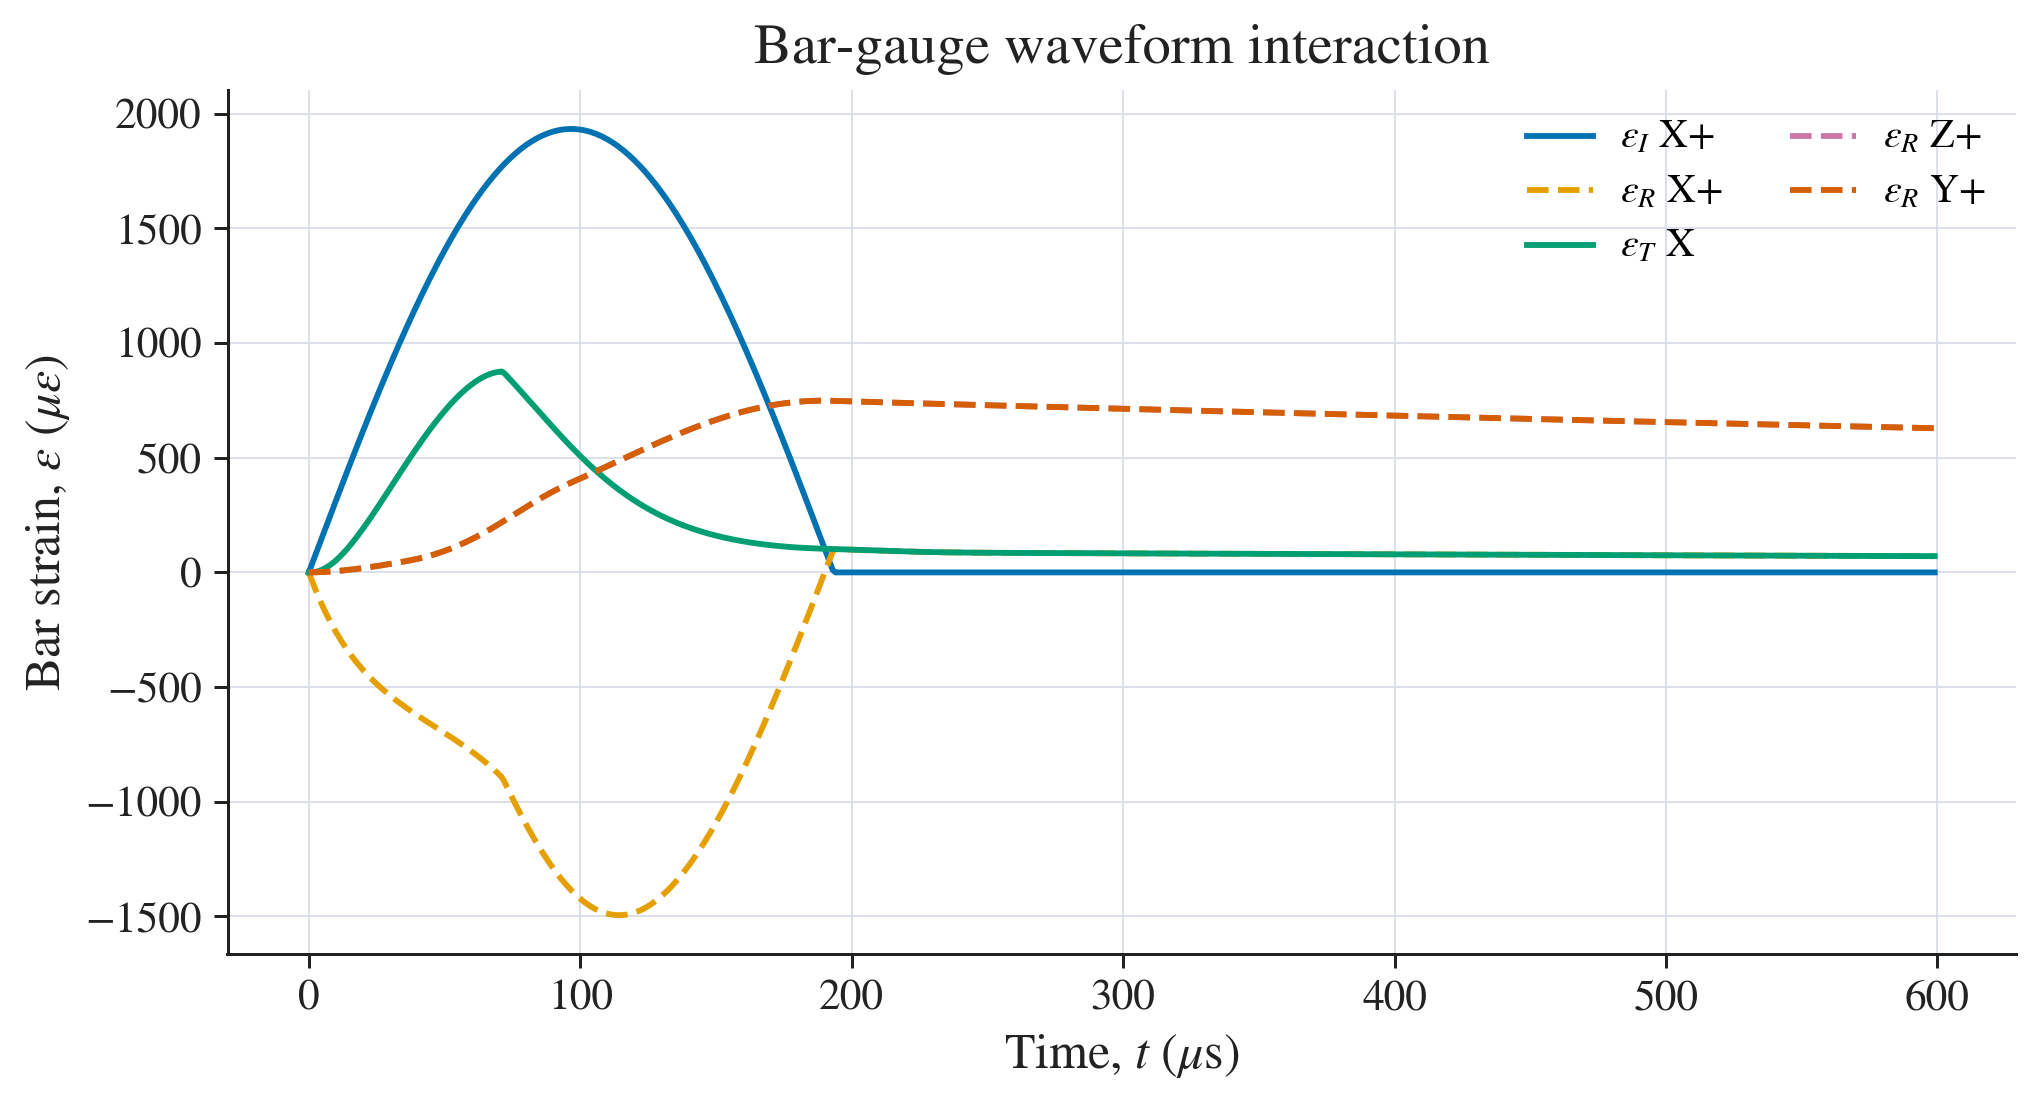
\includegraphics[width=0.92\linewidth]{figures/handbook_modes/mode_1_gas_gun_uniaxial_bar_signals.png}
  \caption{Mode~1 default sandstone case: separated incident, reflected, and transmitted bar-gauge strain histories.}
  \label{fig:mode-1-gas-gun-uniaxial-bar-signals}
\end{figure}

\section{Wave analysis: the three-wave method applied}

Equations \eqref{eq:sig3wave}--\eqref{eq:eps3wave} apply directly:
\begin{empheq}[box=\fbox]{align*}
\sig_x(t) &\;=\; \frac{E_b\Ab}{2\As}\,\bigl[\eps_I(t)+\eps_R(t)+\eps_T(t)\bigr],\\
\epsdot_x(t) &\;=\; \frac{\Cz}{\Ls}\,\bigl[\eps_I(t)-\eps_R(t)-\eps_T(t)\bigr],\\
\eps_x(t) &\;=\; \int_{0}^{t}\!\epsdot_x(\tau)\,d\tau.
\end{empheq}
The output is the dynamic stress--strain curve $\sig_x(\eps_x)$, which is
the primary deliverable of the test. The mean strain rate $\bar\epsdot$ is
taken over the equilibrated portion of the loading branch, typically from
$\eps=\SI{0.2}{\percent}$ to $\eps=\SI{0.8}{\percent}$ for a brittle rock.

\begin{figure}[htbp]
  \centering
  
\includegraphics[width=0.92\linewidth]{figures/handbook_modes/mode_1_gas_gun_uniaxial_stress_strain.png}
  \caption{Mode~1 default sandstone case: axial stress--strain branch from the three-wave reduction.}
  \label{fig:mode-1-gas-gun-uniaxial-stress-strain}
\end{figure}

\section{Lateral response on Y and Z}

Because no active pulse is applied to the lateral axes, the lateral bars
record only the specimen's outward push. Each lateral bar carries a single
outgoing wave $\eps_Y(t)$ or $\eps_Z(t)$, and the lateral dynamic stress is
given by \eqref{eq:lateral-y}--\eqref{eq:lateral-z}. The total lateral stress on each axis is the
sum of the static confining pre-stress and the dynamic contribution.

\begin{figure}[htbp]
  \centering
  
\includegraphics[width=0.92\linewidth]{figures/handbook_modes/mode_1_gas_gun_uniaxial_stress_path.png}
  \caption{Mode~1 default sandstone case: $p$--$q$ stress path for the unconfined baseline.}
  \label{fig:mode-1-gas-gun-uniaxial-stress-path}
\end{figure}

\section{Validity envelope}\label{sec:mode1-envelope}

\begin{itemize}[leftmargin=*]
  \item \textbf{Striker velocity:} $V\le\SI{50}{m/s}$ (slider limit). At
        $V\approx\SI{50}{m/s}$, $\sigpeak\approx\SI{1020}{MPa}$ slightly
        exceeds the current $\sigprop=\SI{1000}{MPa}$ warning threshold.
        Tests intended to stay fully elastic should use
        $V\lesssim\SI{49}{m/s}$, or about $\SI{40}{m/s}$ for conservative
        margin.
  \item \textbf{Pre-stress range:} $0\le\sig_1,\sig_2,\sig_3\le\SI{50}{MPa}$
        per axis in the current digital-twin calibration.
  \item \textbf{Strain rate range:} $\epsdot\sim\SIrange{50}{500}{s^{-1}}$.
\end{itemize}

%==============================================================================
\chapter{Mode 2: Confinement-chamber SHPB}\label{ch:mode2}
%==============================================================================

The confinement-chamber SHPB is the most widely deployed triaxial-SHPB
configuration in the dynamic rock and concrete literature
\cite{ChenSong2011,Zhou2010,ZhangZhao2014,Zhang2022,WangZhang2026}. A cylindrical specimen is held
inside a stiff confining chamber --- typically an oil-filled pressure
vessel sealed by an elastomeric jacket, or a confining sleeve of metal,
PU, or epoxy --- that delivers an axisymmetric lateral pressure
$\sig_2=\sig_3=p_c$. The axial baseline $\sig_1$ is applied through a
hydraulic cylinder acting along the X (loading) line, as in the Monash
Tri-HB (Chapter~\ref{ch:mode3}), while the dynamic pulse is launched by
the same gas-gun bench as in Modes~1 and~3.

The defining contrast with Mode~3 is the \emph{passive} character of the
lateral boundary: the confining medium holds $p_c$ constant throughout
the dynamic event, and there are no lateral bars from which lateral wave
data can be inferred. The arrangement is mechanically simpler than the
six-bar Monash architecture, easier to seal against high $p_c$, and well
suited to applications where the axisymmetric stress state is adequate.
It cannot, however, deliver independent $\sig_2$ and $\sig_3$ or probe
non-axisymmetric stress states: the Lode angle is fixed at
$\theta=0$ (triaxial compression) for the entire test.

\section{Hardware configuration}

\begin{itemize}[leftmargin=*,itemsep=3pt]
  \item \textbf{Specimen geometry.} Cylindrical, with the standard aspect
        ratio $L_s/d_s\in[0.5,1.0]$ (\S\ref{sec:aspect-ratio}). Specimen
        diameter is matched to the bar diameter for the round-bar
        configuration, or chosen with a small clearance for the
        confining jacket.
  \item \textbf{X-axis gas-gun train.} Striker bar (\SI{0.5}{m} standard
        or \SI{1.5}{m} extended), incident bar, transmission bar, and
        absorption bar --- geometrically identical to the X axis of
        Mode~1 and Mode~3.
  \item \textbf{X-axis hydraulic cylinder.} Applies the static axial
        baseline $\sig_1$, in the range \SIrange{0}{50}{MPa} (matched to
        the Monash bench rating). The cylinder reaches equilibrium
        before the gas gun fires; this is the \emph{same} axial loading
        arrangement as in Mode~3.
  \item \textbf{Confining chamber.} A pressure vessel surrounding the
        specimen, sealed by an elastomeric jacket and pressurised with
        hydraulic fluid to $p_c$, in the range
        \SIrange{0}{50}{MPa} (slider cap matched to other modes). The
        chamber wall is stiff steel, much stiffer than the specimen so
        that radial expansion of the specimen produces negligible drop
        in $p_c$ during the dynamic event.
  \item \textbf{Lateral bars: absent.} The chamber wall replaces the
        bar pairs on the Y and Z axes. No lateral wave measurement is
        available; the lateral stress is held at $p_c$ throughout the
        event by the chamber.
\end{itemize}

\section{Loading sequence}

A Mode~2 test proceeds in three sequential phases:

\begin{enumerate}[leftmargin=*,itemsep=3pt]
  \item \textbf{Chamber pressurisation.} The confining fluid is pumped
        to the target $p_c$ at a rate slow enough that no significant
        wave is launched in the specimen
        (\SIrange{30}{60}{s}). The specimen experiences a hydrostatic
        compression of magnitude $p_c$.
  \item \textbf{Axial pre-loading.} The X-axis hydraulic cylinder ramps
        the axial baseline $\sig_1$ to its target value, again slowly,
        producing an additional axial compression of magnitude
        $\sig_1-p_c$ relative to the hydrostatic baseline (so that the
        total axial stress is $\sig_1$ and the lateral is $p_c$).
  \item \textbf{Dynamic pulse.} The gas gun fires the striker bar at
        velocity $V$, producing the standard Hopkinson incident pulse
        on the incident bar. The dynamic increment $\sig_X^{\text{dyn}}$
        adds to the axial baseline; the lateral stress remains at
        $p_c$ throughout (subject to small chamber-compliance
        corrections, \S\ref{sec:mode2-chamber}).
\end{enumerate}

\noindent The total stress history during the dynamic event is therefore
\begin{empheq}[box=\fbox]{align}
  \sig_X^{\text{total}}(t) &\;=\; \sig_1 + \sig_X^{\text{dyn}}(t),  \notag\\
  \sig_Y^{\text{total}}(t) &\;=\; p_c, \label{eq:mode2-superpose}\\
  \sig_Z^{\text{total}}(t) &\;=\; p_c. \notag
\end{empheq}
The lateral stress is constant in time (to leading order); only the
X axis carries dynamic information.

\begin{figure}[htbp]
  \centering
  
\includegraphics[width=0.92\linewidth]{figures/handbook_modes/mode_2_confinement_chamber_stress_history.png}
  \caption{Mode~2 default sandstone case: axial stress history with constant chamber confinement.}
  \label{fig:mode-2-confinement-chamber-stress-history}
\end{figure}

\section{Wave analysis on the active (X) axis}

The X-axis bars carry incident, reflected, and transmitted waves
identically to Modes~1 and~3. The three-wave equations of
\S\ref{sec:three-wave} apply unchanged:
\begin{empheq}[box=\fbox]{align*}
  \sig_X^{\text{dyn}}(t) &\;=\; \frac{E_b\Ab}{2\As}\,\bigl[\eps_I(t)+\eps_R(t)+\eps_T(t)\bigr],\\
  \epsdot_X(t) &\;=\; \frac{\Cz}{\Ls}\,\bigl[\eps_I(t)-\eps_R(t)-\eps_T(t)\bigr],\\
  \eps_X(t) &\;=\; \int_{0}^{t}\!\epsdot_X(\tau)\,d\tau.
\end{empheq}
With a cylindrical specimen and round bars, $\As=\pi d_s^{2}/4$ and
$\Ab=\pi d_b^{2}/4$; for matched diameters, $\As=\Ab$.

\begin{figure}[htbp]
  \centering
  
\includegraphics[width=0.92\linewidth]{figures/handbook_modes/mode_2_confinement_chamber_bar_signals.png}
  \caption{Mode~2 default sandstone case: X-axis bar-gauge histories; no active Y/Z bar diagnostics are available in the chamber mode.}
  \label{fig:mode-2-confinement-chamber-bar-signals}
\end{figure}

\section{Stress invariants and Lode angle}\label{sec:mode2-lode}

Because $\sig_2=\sig_3=p_c$ throughout the test (axisymmetric), the
stress invariants collapse to one-parameter families of $\sig_X$:
\begin{align}
  p(t)   &\;=\; \tfrac{1}{3}\bigl[\sig_X^{\text{total}}(t) + 2p_c\bigr], \\
  q(t)   &\;=\; \bigl|\sig_X^{\text{total}}(t) - p_c\bigr|, \\
  \theta &\;=\; 0 \quad\text{(triaxial compression, fixed).}
\end{align}
A Mode~2 test therefore traces a single radial line in $p$--$q$ space,
parameterised by $p_c$. To explore a different Lode angle requires a
different test (true triaxial, e.g.\ Mode~3 or Mode~5), since the
confinement chamber cannot break the $\sig_2=\sig_3$ symmetry.

\begin{figure}[htbp]
  \centering
  
\includegraphics[width=0.92\linewidth]{figures/handbook_modes/mode_2_confinement_chamber_stress_path.png}
  \caption{Mode~2 default sandstone case: axisymmetric $p$--$q$ path imposed by $\sig_2=\sig_3=p_c$.}
  \label{fig:mode-2-confinement-chamber-stress-path}
\end{figure}

\section{Confinement strengthening}

The Mohr--Coulomb-type strengthening relation
\eqref{eq:peak-strength} applies with $\max(\sig_2,\sig_3)=p_c$:
\begin{equation}
  \sig_{\text{peak}}^{\text{rock,dyn}}
    \;=\; \bigl(\sig_{c0} + k_{\text{conf}}\,p_c\bigr)\cdot\text{DIF},
  \label{eq:mode2-peak-strength}
\end{equation}
the same planning relation that applies to Mode~3 with $\sig_2=\sig_3$
specialised to the hydrostatic case. The axial baseline $\sig_1$ raises
the total axial stress at peak by a constant offset but does not affect
the dynamic peak strength of the rock itself.

\begin{figure}[htbp]
  \centering
  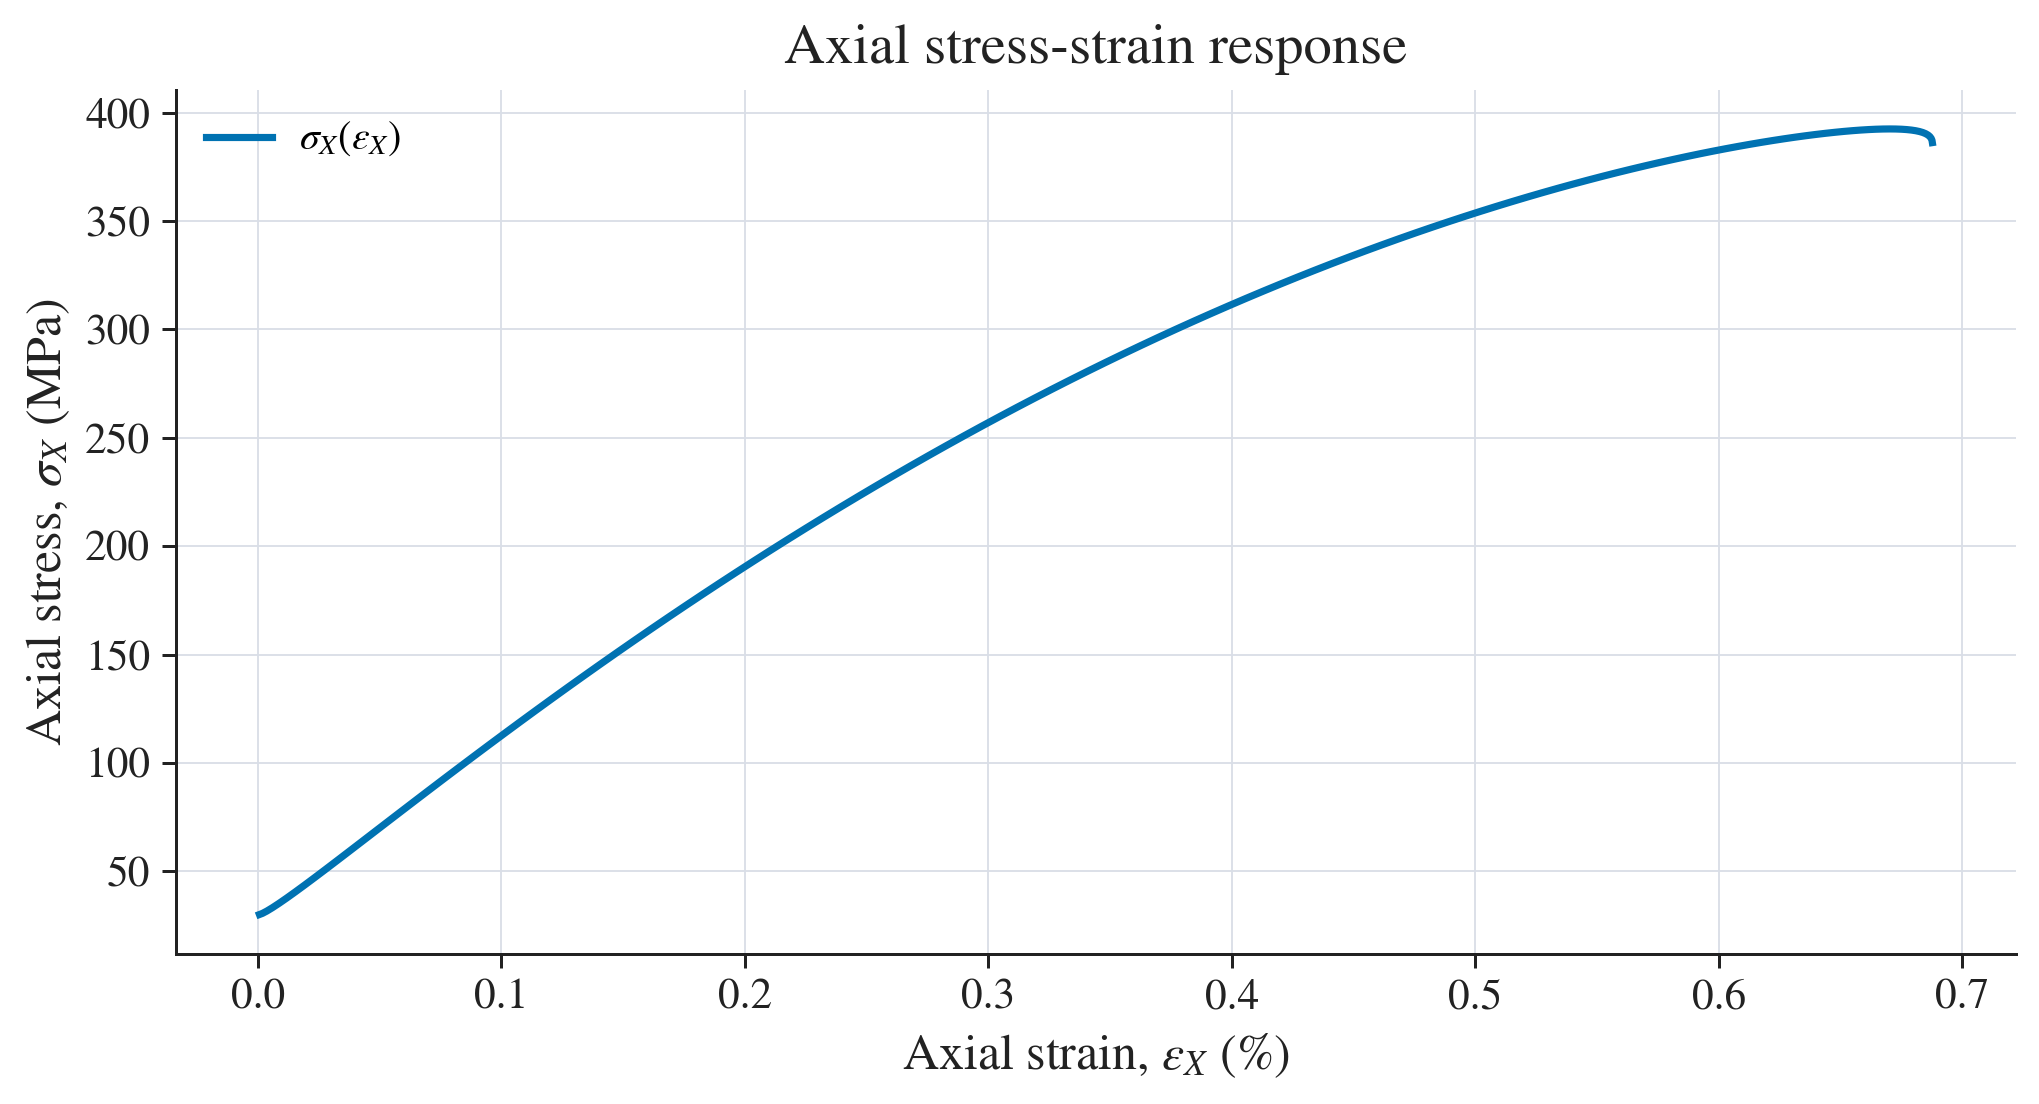
\includegraphics[width=0.92\linewidth]{figures/handbook_modes/mode_2_confinement_chamber_stress_strain.png}
  \caption{Mode~2 default sandstone case: axial stress--strain branch showing confinement-strengthened response.}
  \label{fig:mode-2-confinement-chamber-stress-strain}
\end{figure}

\section{Two parasitic corrections}\label{sec:mode2-chamber}

The simplicity of the chamber configuration comes at the price of two
small-but-real corrections that are absent from the active-bar modes.

\subsection{Chamber compliance}

A finite-stiffness chamber expands slightly when the specimen pushes
outward during the dynamic event, so the effective lateral pressure
deviates from the nominal $p_c$. To leading order,
\begin{equation}
  p_c^{\text{eff}}(t) \;\approx\; p_c + K_c\,\eps_{r,s}(t),
  \label{eq:chamber-compliance}
\end{equation}
where $\eps_{r,s}(t)$ is the radial (lateral) strain of the specimen
and $K_c$ is the effective radial stiffness of the chamber wall per
unit specimen lateral strain. For thick steel chambers $K_c$ is high
enough that this correction is below \SI{1}{\percent} and is normally
neglected; for thin sleeves or fluid-only confinement, it can reach
several percent and should be calibrated against quasi-static
expansion tests of the empty chamber.

\subsection{Jacket parasitic load}

If the elastomeric jacket or metal sleeve carries a portion of the
axial load in parallel with the specimen, the transmission-bar reading
overestimates the specimen force. The correction is
\begin{equation}
  F_s(t) \;=\; F_{\text{bar}}(t) - A_j\,E_j\,\eps_X(t),
  \label{eq:jacket-correction}
\end{equation}
where $A_j$ and $E_j$ are the jacket cross-section and modulus. Soft
elastomer jackets ($E_j\sim\SI{10}{MPa}$) contribute a negligible
correction; metal jackets ($E_j\sim\SI{200}{GPa}$) require explicit
subtraction.

\begin{warningbox}[When the corrections matter]
\textbf{Steel chamber + elastomer jacket} (the most common
arrangement): both corrections are negligible; the bare three-wave
equations are accurate.\\
\textbf{Thin-walled sleeve confinement} (low-cost alternative): chamber
compliance can be \SIrange{5}{15}{\percent} and must be calibrated.\\
\textbf{Metal-jacketed specimen} (used for very weak materials, e.g.\
soils): jacket parasitic load must be subtracted; otherwise the
apparent dynamic strength is overestimated.
\end{warningbox}

\section{Procedure}

\begin{stepbox}[Mode~2 procedure]
\begin{enumerate}[leftmargin=*,itemsep=3pt]
  \item Mount the cylindrical specimen with its jacket inside the
        confining chamber. Verify alignment of the chamber with the
        incident and transmission bar ends.
  \item Pressurise the confining chamber slowly to the target $p_c$
        (default $p_c=\SI{20}{MPa}$). Allow the system to settle
        (\SIrange{30}{60}{s}).
  \item Ramp the X-axis hydraulic cylinder to the target axial baseline
        $\sig_1$ (default $\sig_1=\SI{30}{MPa}$). Allow the system to
        settle.
  \item Record the pre-trigger baseline on the incident, reflected, and
        transmitted bar gauges.
  \item Choose the striker velocity $V$ to deliver the desired
        $\sigpeak=\tfrac{1}{2}\rho_b\Cz V$, using
        \eqref{eq:mode2-peak-strength} as the planning relation.
        Verify $\sigpeak<\sigprop=\SI{1000}{MPa}$.
  \item Trigger the gas gun. Capture all X-axis gauge signals at
        $\ge\SI{1}{MHz}$. Monitor the chamber pressure transducer
        through the event.
  \item Subtract the pre-trigger baselines.
  \item Time-shift each channel to the specimen-face reference.
  \item Verify stress equilibrium $\mathcal{R}(t)<0.05$
        (\eqref{eq:equilibrium}).
  \item Apply the three-wave equations to obtain $\sig_X^{\text{dyn}}(t)$,
        $\epsdot_X(t)$, $\eps_X(t)$.
  \item Apply the chamber-compliance correction
        \eqref{eq:chamber-compliance} if the chamber stiffness warrants
        it; apply the jacket-load correction \eqref{eq:jacket-correction}
        if a metal jacket is used.
  \item Reconstruct the total stresses per \eqref{eq:mode2-superpose}.
  \item Plot $\sig_X^{\text{total}}$ against $\eps_X$, extract peak
        strength and mean strain rate. Compare with the planning
        prediction \eqref{eq:mode2-peak-strength}.
  \item Confirm the maximum bar stress remained below $\sigprop$.
\end{enumerate}
\end{stepbox}

\section{Worked example: sandstone in a steel chamber}

A sandstone specimen ($\sig_{c0}=\SI{80}{MPa}$, $k_{\text{conf}}=4.5$,
$b_{\text{rate}}=0.18$) is to be tested at the digital-twin default
state for the Confinement-chamber mode: $\sig_1=\SI{30}{MPa}$ axial,
$p_c=\sig_2=\sig_3=\SI{20}{MPa}$ confining, with a striker velocity
$V=\SI{20}{m/s}$.

\textbf{Step 1.} Incident pulse amplitude:
\[
  \sigpeak \;=\; \tfrac{1}{2}\rho_b\Cz V \;\approx\; \SI{406}{MPa}.
\]

\textbf{Step 2.} Dynamic peak rock strength from
\eqref{eq:mode2-peak-strength}, assuming
$\bar\epsdot\approx\SI{150}{s^{-1}}$:
\begin{align*}
  \text{DIF} &\;=\; 1 + 0.18\,\log_{10}\!\left(\frac{150}{10^{-5}}\right)
              \;\approx\; 2.29,\\
  \sig_{\text{peak}}^{\text{rock,dyn}}
    &\;=\; (80 + 4.5\times 20)\cdot 2.29 \;\approx\; \SI{390}{MPa}.
\end{align*}

\textbf{Step 3.} Total axial stress at peak:
\[
  \sigpeak^{\text{total}} \;=\; \sig_1 + \sig_{\text{peak}}^{\text{rock,dyn}}
                           \;=\; 30 + 390 \;\approx\; \SI{420}{MPa}.
\]

\textbf{Step 4.} Stress invariants at peak (axisymmetric, $\theta=0$):
\[
  p \;=\; \tfrac{1}{3}(420 + 2\times 20) \;\approx\; \SI{153}{MPa},
  \qquad
  q \;=\; |420-20| \;\approx\; \SI{400}{MPa}.
\]

\textbf{Step 5.} Bar-stress check:
\[
  \sig_{\text{bar}} \;\approx\; \SI{390}{MPa} \;<\; \sigprop=\SI{1000}{MPa}\;\checkmark.
\]

\textbf{Comment.} The dynamic peak rock strength at $p_c=\SI{20}{MPa}$
is identical to that computed for Mode~3 in the worked example below
(Chapter~\ref{ch:mode3}) at the same $\max(\sig_2,\sig_3)=\SI{20}{MPa}$.
The two modes therefore give equivalent peak-strength predictions when
the Monash Tri-HB happens to be operated with $\sig_2=\sig_3$. What
Mode~2 \emph{cannot} reproduce is the response under
$\sig_2\neq\sig_3$ (e.g., the default Mode~3 state $\sig_2=20$, $\sig_3=15$
with $\theta>0$): for that, the active-bar architecture of Mode~3 is
required.

\section{Validity envelope}

\begin{itemize}[leftmargin=*]
  \item \textbf{Striker velocity:} the Streamlit slider permits
        $V\le\SI{50}{m/s}$; the bar-limit warning should remain clear, so
        $V\lesssim\SI{49}{m/s}$ is the practical elastic upper bound for
        the default bar constants.
  \item \textbf{Confining pressure:} $0\le p_c\le\SI{50}{MPa}$ for the
        digital-twin slider; the physical chamber rating may permit
        higher values (\SIrange{100}{300}{MPa} in published rigs).
  \item \textbf{Axial baseline:} $0\le\sig_1\le\SI{50}{MPa}$.
  \item \textbf{Strain rate range:} $\epsdot\sim\SIrange{50}{500}{s^{-1}}$.
  \item \textbf{Lode angle:} fixed at $\theta=0$. For research questions
        requiring $\theta>0$, use Mode~3 or Mode~5.
\end{itemize}


%==============================================================================
\chapter{Mode 3: Monash Tri-HB --- gas-gun coupled static--dynamic triaxial loading}\label{ch:mode3}
%==============================================================================

This mode is the signature physical capability of the Monash Tri-HB
facility (\S\ref{sec:monash-trihb}). The gas-gun hardware of Mode~1 is
retained, but active triaxial confining pre-stress is applied on the Y and Z
axes through the lateral hydraulic cylinders \emph{before} the striker bar
fires. The specimen therefore experiences a quasi-static triaxial stress
state plus a uniaxial dynamic increment along X --- the loading regime
representative of an in-situ rockmass struck by a blast or seismic wave
\cite{Liu2019,Zhang2019Tri}.

\section{Hardware configuration}

The bench and bar geometry are identical to Mode~1: striker
(\SI{0.5}{m} for the standard configuration; \SI{1.5}{m} for the Monash
extended striker), incident bar (\SI{2.5}{m}), transmission bar (\SI{2}{m}),
and absorption bar (\SI{0.5}{m}) along X. What distinguishes Mode~3 from
Mode~1 is the \emph{active} role of the lateral train:

\begin{itemize}[leftmargin=*,itemsep=3pt]
  \item \textbf{Y-axis bars} ($\pm Y$, four bars of \SI{2}{m}) loaded by
        a horizontal hydraulic cylinder to apply $\sig_2$ on the specimen.
  \item \textbf{Z-axis bars} ($\pm Z$, four bars of \SI{2}{m}) loaded by
        a vertical hydraulic cylinder to apply $\sig_3$ on the specimen.
  \item \textbf{X-axis hydraulic cylinder} optionally applies an axial
        baseline $\sig_1$.
  \item \textbf{Reaction frames} (six high-strength steel) carry the
        static pre-load and isolate the gas-gun bench from the cylinder
        line of action.
\end{itemize}

\noindent The four lateral output bars (one bonded to each of the four
lateral faces of the cubic specimen: $\pm Y$ and $\pm Z$) record the
specimen's lateral wave response in real time, allowing the dynamic Y and
Z stresses to be inferred from \eqref{eq:lateral-y}--\eqref{eq:lateral-z}.
The hydraulic cylinders are servo-controlled and reach equilibrium with
the specimen before the gas gun is triggered.

\section{Loading sequence and superposition}

A Mode~3 test proceeds in two distinct phases:

\begin{enumerate}[leftmargin=*,itemsep=3pt]
  \item \textbf{Quasi-static pre-loading.} The hydraulic cylinders ramp
        $\sig_1,\sig_2,\sig_3$ to their target values over
        \SIrange{30}{60}{s}, slow enough that the bars deform elastically
        and no stress wave is generated. The strain gauges record this as
        a low-frequency baseline.
  \item \textbf{Dynamic pulse.} The gas gun fires the striker bar at
        velocity $V$, producing the standard Hopkinson incident pulse
        $\sigpeak=\tfrac{1}{2}\rho_b\Cz V$ on the incident bar. The
        dynamic pulse reaches the specimen and is processed by the
        three-wave method exactly as in Mode~1.
\end{enumerate}

\noindent Because the two phases are temporally separated, the
specimen-stress response is the linear superposition of the static
pre-stress and the dynamic increment, per \eqref{eq:superpose-static}:
\begin{align}
  \sig_X^{\text{total}}(t) &\;=\; \sig_1 + \sig_X^{\text{dyn}}(t),  \notag \\
  \sig_Y^{\text{total}}(t) &\;=\; \sig_2 + \sig_Y^{\text{dyn}}(t),  \\
  \sig_Z^{\text{total}}(t) &\;=\; \sig_3 + \sig_Z^{\text{dyn}}(t).  \notag
\end{align}
On the X axis $\sig_X^{\text{dyn}}$ is the active dynamic stress driven by
the striker; on Y and Z, $\sig_Y^{\text{dyn}}$ and $\sig_Z^{\text{dyn}}$
are the small Poisson-coupled lateral responses
$\sig_{\text{lat}}^{\text{dyn}}\approx -\nu\sig_X^{\text{dyn}}$ measured on
the lateral output bars.

\begin{figure}[htbp]
  \centering
  
\includegraphics[width=0.92\linewidth]{figures/handbook_modes/mode_3_monash_tri_hb_stress_history.png}
  \caption{Mode~3 default sandstone case: total stress histories after superposing independent static pre-stress and the gas-gun dynamic increment.}
  \label{fig:mode-3-monash-tri-hb-stress-history}
\end{figure}

\subsection{Why the bar gauges do not record the pre-stress}

As discussed in \S\ref{sec:prestress}, the static pre-stress is held by the
hydraulic cylinders and is subtracted as the pre-event baseline at data
acquisition. The wave-analysis equations operate exclusively on the dynamic
component; the static pre-stress is reintroduced at the reporting stage
through the superposition above. This is the same convention used in
Modes~1 and~3--5.

\section{Wave analysis on the active (X) axis}

The three-wave equations of \S\ref{sec:three-wave} apply unchanged:
\begin{empheq}[box=\fbox]{align*}
  \sig_X^{\text{dyn}}(t) &\;=\; \frac{E_b\Ab}{2\As}\,\bigl[\eps_I(t)+\eps_R(t)+\eps_T(t)\bigr],\\
  \epsdot_X(t) &\;=\; \frac{\Cz}{\Ls}\,\bigl[\eps_I(t)-\eps_R(t)-\eps_T(t)\bigr],\\
  \eps_X(t) &\;=\; \int_{0}^{t}\!\epsdot_X(\tau)\,d\tau.
\end{empheq}
The bars remain the diagnostic instruments; the constitutive interpretation
of $(\sig_X^{\text{total}},\eps_X)$ must now account for the confining
pre-stress on Y and Z via a multiaxial failure surface (Chapter~\ref{ch:wavedamage}).

\begin{figure}[htbp]
  \centering
  
\includegraphics[width=0.92\linewidth]{figures/handbook_modes/mode_3_monash_tri_hb_bar_signals.png}
  \caption{Mode~3 default sandstone case: active X-axis Hopkinson signals together with lateral output-bar responses.}
  \label{fig:mode-3-monash-tri-hb-bar-signals}
\end{figure}

\section{Confinement strengthening}\label{sec:mode3-strengthening}

The principal value of Mode~3 over Mode~1 is the strengthening induced by
active confinement. For low-to-moderate confining pressure, the dynamic
peak rock strength follows the Mohr--Coulomb-type relation
\eqref{eq:peak-strength}:
\begin{equation}
  \sig_{\text{peak}}^{\text{rock,dyn}}
    \;=\; \bigl[\sig_{c0} + k_{\text{conf}}\,\max(\sig_2,\sig_3)\bigr]\cdot\text{DIF},
  \label{eq:mode3-peak}
\end{equation}
where $k_{\text{conf}}$ is the confinement coefficient and DIF the rate
factor of \eqref{eq:DIF}. This is the equation underpinning the Liu et al.\
\cite{Liu2019} sandstone dataset and forms the planning relation for
selecting striker velocity and pre-stress combinations.

\begin{conceptbox}[Why $\sig_2$ and $\sig_3$ strengthen but $\sig_1$ does not]
The axial baseline $\sig_1$ is collinear with the dynamic pulse: it shifts
the total axial stress curve upward without altering the deviatoric stress
the specimen must resist. The lateral pre-stresses $\sig_2$ and $\sig_3$,
on the other hand, are perpendicular to the loading axis: they reduce the
deviatoric stress at any given $\sig_X$ and therefore raise the dynamic
peak through the Mohr--Coulomb mechanism. Exercise~7 of
Appendix~\ref{app:exercises} explores this asymmetry quantitatively.
\end{conceptbox}

\begin{figure}[htbp]
  \centering
  
\includegraphics[width=0.92\linewidth]{figures/handbook_modes/mode_3_monash_tri_hb_stress_path.png}
  \caption{Mode~3 default sandstone case: $p$--$q$ stress path under independent triaxial pre-stress.}
  \label{fig:mode-3-monash-tri-hb-stress-path}
\end{figure}

\section{Procedure}

\begin{stepbox}[Mode~3 procedure]
\begin{enumerate}[leftmargin=*,itemsep=3pt]
  \item Place the cubic specimen between the two X bars. Bring the four
        lateral output bars on Y and Z into contact with the specimen
        faces; verify alignment.
  \item Set the target confining pre-stresses $\sig_2$ and $\sig_3$ on the
        Y and Z hydraulic cylinders. Optionally set an axial baseline
        $\sig_1$ on the X cylinder. Ramp slowly
        (\SIrange{30}{60}{s}) and allow the system to settle.
  \item Record the pre-trigger baseline on all bar gauges (incident,
        reflected, transmitted, and the four lateral output gauges
        Y$_1$, Y$_2$, Z$_1$, Z$_2$).
  \item Choose the striker velocity $V$ to deliver the desired dynamic
        peak $\sigpeak=\tfrac{1}{2}\rho_b\Cz V$, using \eqref{eq:mode3-peak}
        as the planning relation. Verify $\sigpeak<\sigprop=\SI{1000}{MPa}$.
  \item Trigger the gas gun. Capture all gauge signals at sampling rates
        $\ge\SI{1}{MHz}$.
  \item Subtract the pre-trigger baseline from each channel (this removes
        the static pre-stress from the recorded dynamic signals).
  \item Time-shift each channel to the specimen-face reference.
  \item Verify stress equilibrium $\mathcal{R}(t)<0.05$ per
        \eqref{eq:equilibrium}.
  \item Apply the three-wave equations to obtain $\sig_X^{\text{dyn}}(t)$,
        $\epsdot_X(t)$, and $\eps_X(t)$.
  \item From the lateral output bars compute the Poisson-coupled responses
        $\sig_Y^{\text{dyn}}(t)$ and $\sig_Z^{\text{dyn}}(t)$ via
        \eqref{eq:lateral-y}--\eqref{eq:lateral-z}.
  \item Add the static pre-stresses back per \eqref{eq:superpose-static} to
        obtain the total stress histories $\sig_X^{\text{total}}$,
        $\sig_Y^{\text{total}}$, $\sig_Z^{\text{total}}$.
  \item Plot $\sig_X^{\text{total}}$ against $\eps_X$, extract the peak
        strength and mean strain rate. Compare with the planning
        prediction~\eqref{eq:mode3-peak}.
  \item Confirm the maximum bar stress remained below $\sigprop$.
\end{enumerate}
\end{stepbox}

\section{Worked example: sandstone under triaxial pre-stress}

A sandstone specimen ($\sig_{c0}=\SI{80}{MPa}$, $k_{\text{conf}}=4.5$,
$b_{\text{rate}}=0.18$) is to be tested at the digital-twin default
pre-stress state for the Monash Tri-HB mode, $\sig_1=\SI{30}{MPa}$ axial,
$\sig_2=\SI{20}{MPa}$, $\sig_3=\SI{15}{MPa}$ (note that $\sig_2$ and
$\sig_3$ may be set independently in this mode), with a striker velocity
$V=\SI{20}{m/s}$.

\textbf{Step 1.} Incident pulse amplitude from the Hopkinson identity:
\[
  \sigpeak \;=\; \tfrac{1}{2}\rho_b\Cz V
              \;=\; \tfrac{1}{2}(7850)(5172)(20) \cdot 10^{-6}
              \;\approx\; \SI{406}{MPa}.
\]

\textbf{Step 2.} Estimated dynamic peak rock strength from
\eqref{eq:mode3-peak}, taking $\max(\sig_2,\sig_3)=\SI{20}{MPa}$ and
assuming $\bar\epsdot\approx\SI{150}{s^{-1}}$:
\begin{align*}
  \text{DIF} &\;=\; 1 + 0.18\,\log_{10}\!\left(\frac{150}{10^{-5}}\right)
                \;\approx\; 2.29, \\
  \sig_{\text{peak}}^{\text{rock,dyn}}
    &\;=\; (80 + 4.5\times 20)\cdot 2.29
    \;\approx\; \SI{390}{MPa}.
\end{align*}

\textbf{Step 3.} Total axial stress at peak:
\[
  \sigpeak^{\text{total}} \;=\; \sig_1 + \sig_{\text{peak}}^{\text{rock,dyn}}
                          \;=\; 30 + 390 \;\approx\; \SI{420}{MPa}.
\]

\textbf{Step 4.} Bar-stress check. The bar must transmit a stress equal to
$\sig_{\text{peak}}^{\text{rock,dyn}}\cdot \As/\Ab$. With matched
\SI{50}{mm} cubic specimen and square bars, $\As/\Ab=1$:
\[
  \sig_{\text{bar}} \;\approx\; \SI{390}{MPa}
                    \;<\; \sigprop=\SI{1000}{MPa}\;\checkmark.
\]

\textbf{Step 5.} Comparison with Mode~1 (same striker, no confinement).
The unconfined dynamic peak would be only
\[
  \sig_{\text{peak},0}^{\text{rock,dyn}}
    \;=\; \sig_{c0}\cdot\text{DIF}
    \;\approx\; 80\cdot 2.29 \;\approx\; \SI{183}{MPa},
\]
a factor of $\sim 2.1$ below the confined value. This is the dynamic
analogue of the well-known confinement strengthening of quasi-static
triaxial tests; the Monash Tri-HB allows it to be measured at high strain
rate \cite{Liu2019}.

\begin{figure}[htbp]
  \centering
  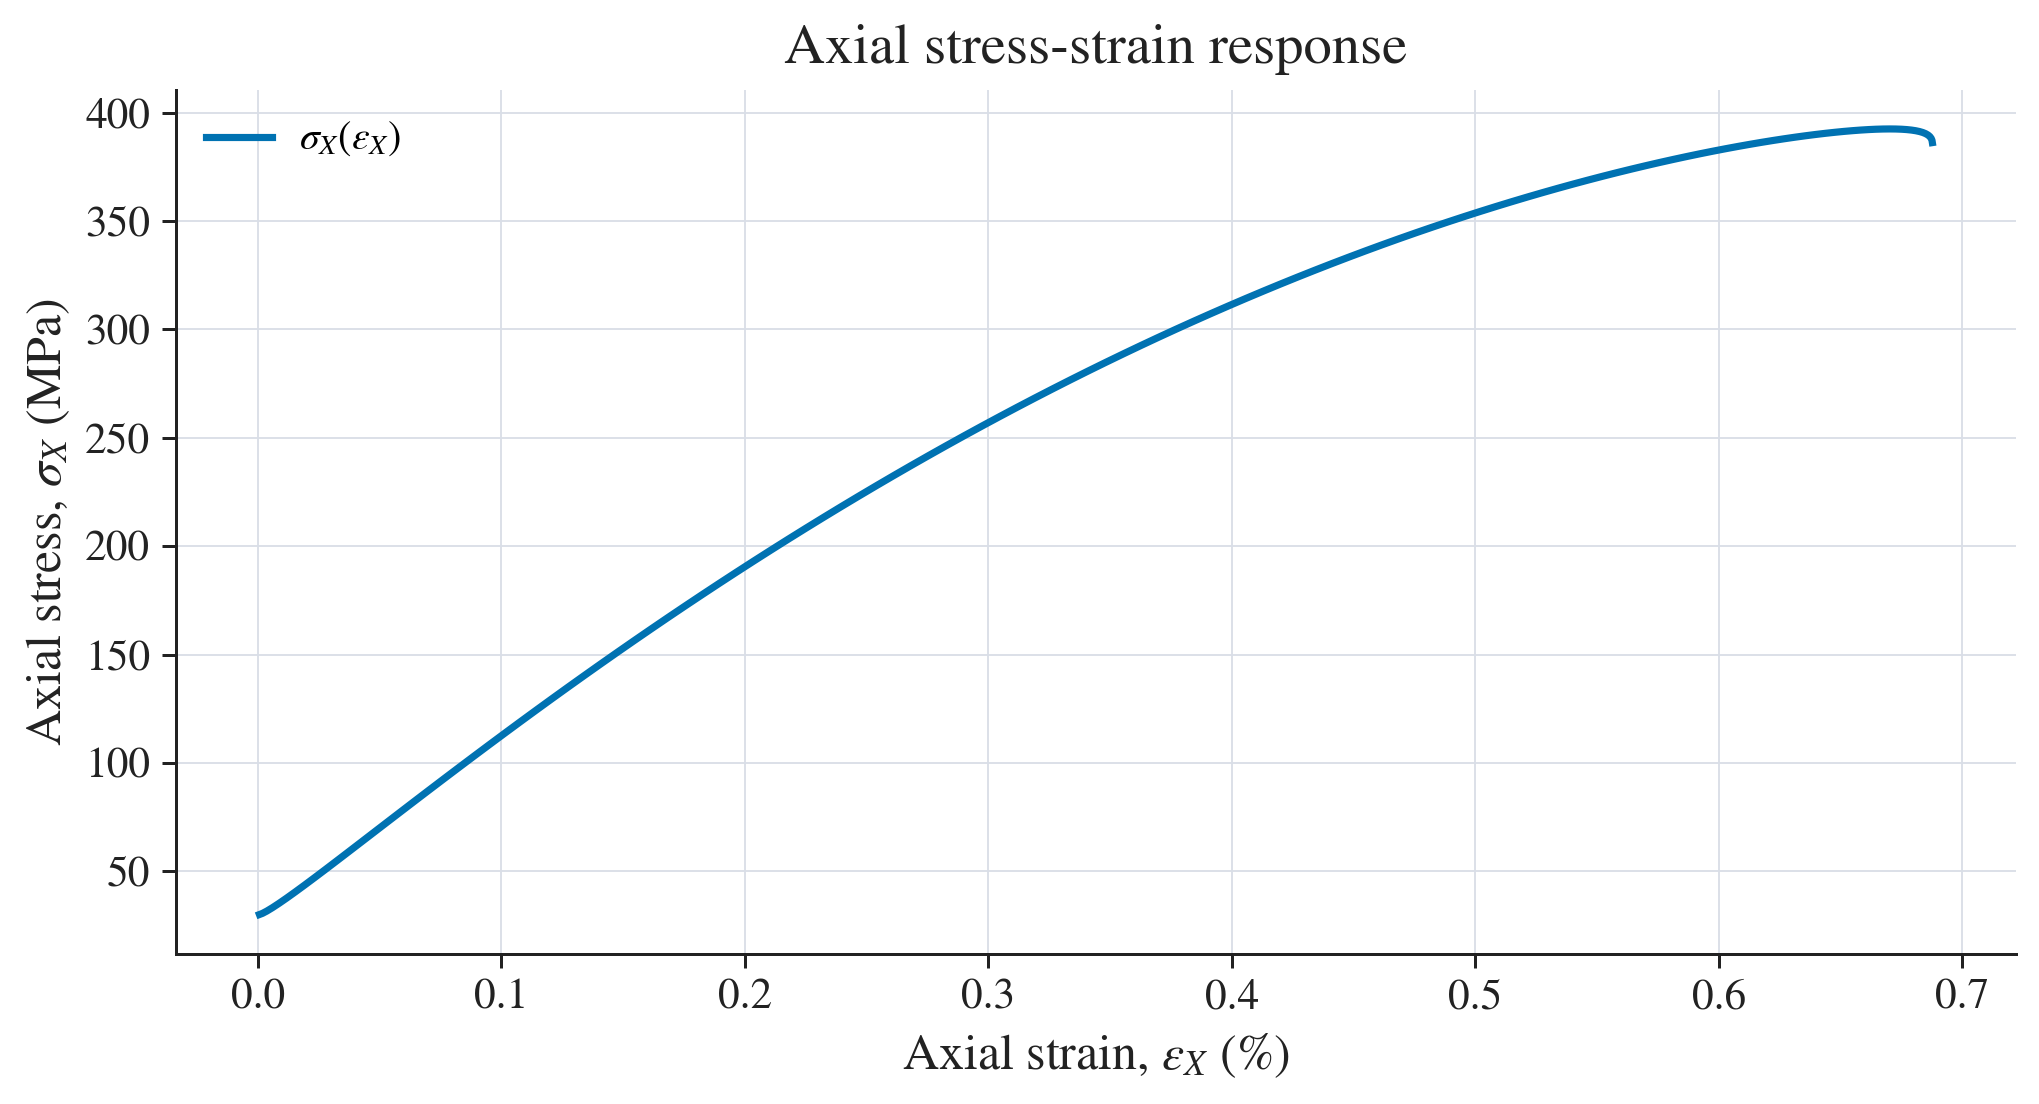
\includegraphics[width=0.92\linewidth]{figures/handbook_modes/mode_3_monash_tri_hb_stress_strain.png}
  \caption{Mode~3 default sandstone case: axial stress--strain branch for the gas-gun true-triaxial configuration.}
  \label{fig:mode-3-monash-tri-hb-stress-strain}
\end{figure}

\section{Validity envelope}

\begin{itemize}[leftmargin=*]
  \item \textbf{Striker velocity:} the Streamlit slider permits
        $V\le\SI{50}{m/s}$; keep the bar-limit warning clear
        ($V\lesssim\SI{49}{m/s}$ for the default bar constants; see
        \S\ref{sec:mode1-envelope}).
  \item \textbf{Confining pre-stress range:}
        $0\le\sig_2,\sig_3\le\SI{50}{MPa}$ per axis (slider cap of the
        current digital-twin calibration; matched to the
        \SI{50}{MPa} hydraulic-cylinder rating of the Monash bench).
  \item \textbf{Axial baseline:} $0\le\sig_1\le\SI{50}{MPa}$. The total
        axial stress $\sig_1+\sig_X^{\text{dyn}}$ must remain within the
        constitutive validity range of the chosen failure model.
  \item \textbf{Strain rate range:} $\epsdot\sim\SIrange{50}{500}{s^{-1}}$.
  \item \textbf{Confinement vs strain rate.} Increasing confinement
        $\sig_2,\sig_3$ raises the dynamic peak strength but also reduces
        the achieved strain rate at a given striker velocity, because the
        specimen deforms less before failure. The two parameters should be
        swept independently for a complete constitutive characterisation.
\end{itemize}

%==============================================================================
\chapter{Mode 4: Electromagnetic uniaxial impact}\label{ch:mode4}
%==============================================================================

The electromagnetic uniaxial mode replaces the gas gun and striker bar with
a capacitor-bank-driven coil that produces a Lorentz force on a flyer plate
(or directly on the bar end), launching a stress pulse into a single
incident bar. The data-reduction equations are identical to Mode~1, and the
pulse shape is the same smooth half-sine; the distinguishing feature is the
\emph{independent} control of pulse amplitude and duration, which the
gas-gun drive cannot provide.

\section{Hardware differences from Mode~1}

\begin{itemize}[leftmargin=*,itemsep=2pt]
  \item \textbf{Pulse generator:} capacitor bank discharged through a primary
        coil produces a Lorentz force on the flyer/bar end.
  \item \textbf{Bars:} square cross-section \SI{50}{mm}$\times$\SI{50}{mm}
        ($\Ab=\SI{2500}{mm^{2}}$) by default, for flat contact with cubic
        specimens. Editable in the Step~1 sidebar.
  \item \textbf{Pre-stress:} same as Mode~1.
\end{itemize}

\section{The half-sine pulse}\label{sec:halfsine}

Both the pulse-shaped gas-gun modes and the electromagnetic generator produce
a clean half-sine pulse:
\begin{empheq}[box=\fbox]{equation}
  \sig_I(t) \;=\; \sigpeak\,\sin\!\left(\frac{\pi t}{\tau}\right),
  \qquad 0\le t\le\tau.
  \label{eq:halfsine}
\end{empheq}
The difference between the two drives is not the pulse \emph{shape} but the
control of its parameters. In the gas-gun modes the peak amplitude
$\sigpeak=\tfrac12(E_b/\Cz)V$ and the duration $\tau=2L_{\text{striker}}/\Cz$
are both fixed by the striker velocity and geometry. In the electromagnetic
modes the peak amplitude $\sigpeak$ and duration $\tau$ are \emph{independently}
tuneable through the capacitor charging voltage and the circuit inductance,
respectively. This decoupling is the chief advantage of the electromagnetic
system: students can sweep the strain-rate axis by varying $\tau$ alone,
holding $\sigpeak$ fixed, a controlled experiment that the gas gun cannot
provide because there $\sigpeak$ and $\tau$ are linked through the striker
geometry and velocity.

\begin{figure}[htbp]
  \centering
  
\includegraphics[width=0.92\linewidth]{figures/handbook_modes/mode_4_em_uniaxial_stress_history.png}
  \caption{Mode~4 default sandstone case: stress history generated by a single electromagnetic half-sine pulse.}
  \label{fig:mode-4-em-uniaxial-stress-history}
\end{figure}

\subsection{Frequency content of the half-sine}

A perfectly rectangular pulse contains arbitrarily high-frequency Fourier
components, which travel at slightly different speeds in the bar and
develop into spurious oscillations as the pulse propagates
(\S\ref{sec:dispersion}). The Fourier transform of the half-sine
\eqref{eq:halfsine} is
\begin{equation}
  |\widehat{\sig}_I(\omega)|
    \;=\; \frac{\sigpeak\,\pi}{|\omega^{2}\tau^{2}-\pi^{2}|}\,
          \bigl|1+\cos(\omega\tau)\bigr|^{1/2},
\end{equation}
whose energy is concentrated near the fundamental frequency
$f_0=1/(2\tau)$ with rapidly decaying higher harmonics. Less high-frequency
content means less dispersion and cleaner signals. A half-sine pulse also
reaches dynamic stress equilibrium faster than a rectangular pulse of the
same amplitude, because its smooth rise gives the specimen time to
reverberate internally before peak stress is reached --- a property
critical for brittle materials.

\begin{figure}[htbp]
  \centering
  
\includegraphics[width=0.92\linewidth]{figures/handbook_modes/mode_4_em_uniaxial_bar_signals.png}
  \caption{Mode~4 default sandstone case: bar-gauge histories produced by the smooth half-sine electromagnetic drive.}
  \label{fig:mode-4-em-uniaxial-bar-signals}
\end{figure}

\section{Step-by-step procedure}

\begin{stepbox}[Mode~4 procedure]
\begin{enumerate}[leftmargin=*,itemsep=3pt]
  \item Apply static pre-stress $\sig_1$ (axial), $\sig_2$, $\sig_3$
        (confining) via the three independent servo-cylinders. Record
        baseline strain on all gauges and let the system settle
        (\SIrange{30}{60}{s}).
  \item Charge the capacitor bank to the voltage required for the desired
        $\sigpeak$, and set the circuit inductance for the desired $\tau$.
  \item Trigger the pulse generator. Capture all bar gauge signals at
        sampling rates $\ge\SI{1}{MHz}$.
  \item Subtract the pre-trigger baseline from each channel (this is what
        removes the static pre-stress from the recorded signal:
        \S\ref{sec:prestress}).
  \item Time-shift each channel to the specimen-face reference: incident
        gauge forward by $L_g/\Cz$, reflected backward by $L_g/\Cz$, etc.
  \item Verify stress equilibrium: $\mathcal{R}(t)<0.05$ per
        \eqref{eq:equilibrium}.
  \item Apply the three-wave equations to obtain $\sig_x^{\text{dyn}}(t)$,
        $\epsdot_x(t)$, $\eps_x(t)$.
  \item Add the static $\sig_1$ baseline to obtain the total axial stress
        per \eqref{eq:superpose-static}.
  \item Plot $\sig_x^{\text{total}}$ against $\eps_x$, extract the peak
        strength and mean strain rate.
  \item Confirm that the maximum bar stress remained below
        $\sigprop=\SI{1000}{MPa}$.
\end{enumerate}
\end{stepbox}

\begin{figure}[htbp]
  \centering
  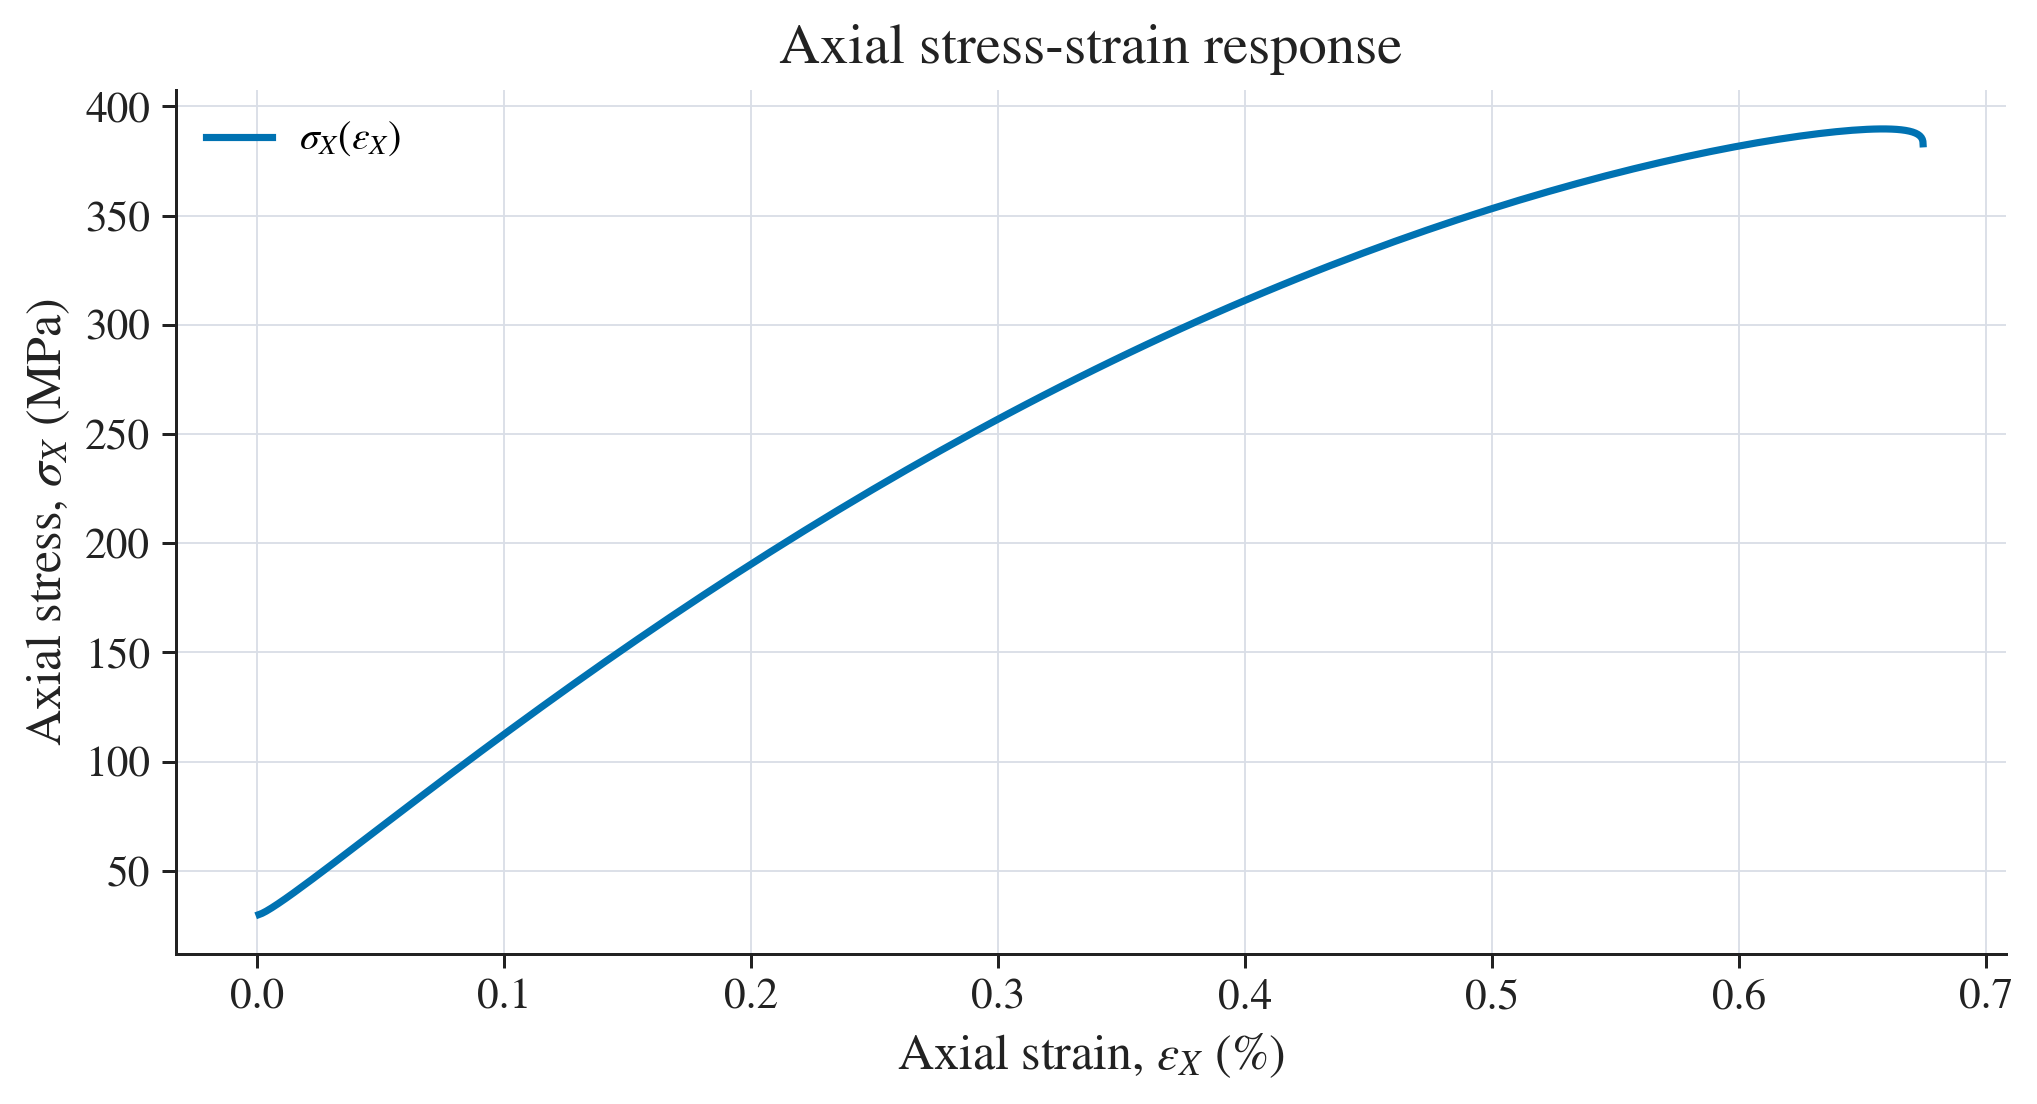
\includegraphics[width=0.92\linewidth]{figures/handbook_modes/mode_4_em_uniaxial_stress_strain.png}
  \caption{Mode~4 default sandstone case: axial stress--strain branch under electromagnetic uniaxial loading.}
  \label{fig:mode-4-em-uniaxial-stress-strain}
\end{figure}

\begin{figure}[htbp]
  \centering
  
\includegraphics[width=0.92\linewidth]{figures/handbook_modes/mode_4_em_uniaxial_stress_path.png}
  \caption{Mode~4 default sandstone case: $p$--$q$ stress path for the one-sided electromagnetic pulse with default pre-stress.}
  \label{fig:mode-4-em-uniaxial-stress-path}
\end{figure}

\section{Worked example: sandstone with triaxial pre-stress}

Consider a sandstone specimen with quasi-static UCS $\sig_{c0}\approx
\SI{80}{MPa}$, Mohr--Coulomb slope $k_{\text{conf}}\approx 4.5$, and
rate-hardening coefficient $b_{\text{rate}}=0.18$, to be tested at the
digital-twin default pre-stress state for the electromagnetic modes,
$\sig_1=\SI{30}{MPa}$ axial baseline, $\sig_2=\SI{20}{MPa}$,
$\sig_3=\SI{15}{MPa}$, at a target strain rate
$\bar\epsdot\approx\SI{200}{s^{-1}}$.

\textbf{Step 1.} Predicted dynamic peak strength of the specimen, using
\eqref{eq:peak-strength} and \eqref{eq:DIF}, with
$\max(\sig_2,\sig_3)=\SI{20}{MPa}$:
\begin{align*}
  \text{DIF} &\;=\; 1 + 0.18\,\log_{10}\!\left(\frac{200}{10^{-5}}\right)
              \;\approx\; 2.31,\\[2pt]
  \sigpeak^{\text{rock,dyn}}
    &\;=\; \bigl(\sig_{c0}+k_{\text{conf}}\max(\sig_2,\sig_3)\bigr)\cdot\text{DIF} \\
    &\;=\; \bigl(80 + 4.5\times 20\bigr)\text{ MPa}\cdot 2.31
    \;\approx\; \SI{393}{MPa}.
\end{align*}

\textbf{Step 2.} Total axial stress at peak:
\begin{equation*}
  \sigpeak^{\text{total}} \;=\; \sig_1 + \sigpeak^{\text{rock,dyn}}
                          \;=\; 30 + 393 \;\approx\; \SI{423}{MPa}.
\end{equation*}

\textbf{Step 3.} Required bar stress. The bar carries only the dynamic
component (the static $\sig_1$ being held by the cylinder); with $\As=\Ab$
for a \SI{50}{mm} cubic specimen between matched square bars,
\begin{equation*}
  \sig_{\text{bar}} \;=\; \sigpeak^{\text{rock,dyn}}\cdot\frac{\As}{\Ab}
                    \;\approx\; \SI{393}{MPa}.
\end{equation*}

\textbf{Conclusion.} \SI{393}{MPa} is well below the \SI{1000}{MPa} bar
proportional limit ($\sim 39\%$ of $\sigprop$): safe to proceed. Charge
the capacitor for $\sigpeak\approx\SI{500}{MPa}$ (allowing a margin above
\SI{393}{MPa} to drive the specimen through peak), choose
$\tau\approx\SI{200}{\micro s}$ to achieve the target strain rate. The
digital twin reports a total axial stress reaching $\sim\SI{423}{MPa}$ on
the $\sig_X$ trace, comprising the static $\sig_1=\SI{30}{MPa}$ plus the
dynamic peak.

%==============================================================================
\chapter{Mode 5: Electromagnetic asynchronous triaxial impact}\label{ch:mode5}
%==============================================================================

This mode uses one, two, or three of the positive-axis electromagnetic
generators to apply one-sided pulses along $+X$, $+Y$, and $+Z$. In the full
triaxial setting each active axis has an independently specified amplitude,
and the Y and Z pulses can be delayed relative to X. It enables the study of
how the \emph{order} of multi-axis loading affects material failure --- a
question that classical uniaxial Hopkinson testing cannot address.

\section{Hardware configuration}

Three pulse generators fire on three orthogonal incident bars. The remaining
three bars (at the $-X$, $-Y$, $-Z$ ends) act as transmission/output bars
and remain passive. In this mode, each of the three positive-axis directions
hosts its own three-wave problem; the negative-axis directions show
transmitted signals only.

In the Streamlit interface the active-axis selector exposes X, X+Y, and
X+Y+Z. The synchronous shortcut sets $\Delta t_y=\Delta t_z=0$, while the
asynchronous controls allow Y/Z delays from \SIrange{0}{500}{\micro s}.

\section{The time-delay concept}

Let pulse $i\in\{x,y,z\}$ be
\begin{equation}
  \sig_{I,i}(t) \;=\; A_i\,\sin\!\left(\frac{\pi(t-\Delta t_i)}{\tau}\right),
  \qquad \Delta t_i \le t \le \Delta t_i+\tau.
  \label{eq:async-pulse}
\end{equation}
Setting $\Delta t_x=0$, $\Delta t_y=\SI{50}{\micro s}$,
$\Delta t_z=\SI{100}{\micro s}$ produces sequential triaxial loading: the
specimen first experiences uniaxial dynamic compression along X, then
biaxial after \SI{50}{\micro s}, then triaxial after \SI{100}{\micro s}.

\begin{conceptbox}[Why ordering matters]
Brittle failure in rock and concrete is path-dependent
\cite{ZhaoKaiser2009}. Cracks initiated in one loading direction can be
either suppressed (if confinement arrives quickly) or allowed to propagate
(if confinement arrives late). Asynchronous loading isolates this effect
from the synchronous case, producing data on the fundamental question of
whether dynamic constitutive models require an explicit stress-path term.

Steps~2--3 of the integrated workspace (Chapter~\ref{ch:wavedamage}) turn
this informal question into a quantitative one through the normalised-delay
parameter $\Delta t^{\ast}=\Delta t/t_{\text{travel}}$ and the
regime-classifier map of \S\ref{sec:wave-regime}.
\end{conceptbox}

\begin{figure}[htbp]
  \centering
  
\includegraphics[width=0.92\linewidth]{figures/handbook_modes/mode_5_em_async_triaxial_stress_history.png}
  \caption{Mode~5 default sandstone case: three-axis electromagnetic stress histories with the default zero-delay setting.}
  \label{fig:mode-5-em-async-triaxial-stress-history}
\end{figure}

\section{Three-wave analysis on each axis}

Because each axis carries its own incident wave, each axis is analysed with
the full three-wave method independently:
\begin{empheq}[box=\fbox]{equation}
  \sig_i(t) \;=\; \frac{E_b\Ab}{2\As}\,
    \bigl[\eps_{I,i}(t) + \eps_{R,i}(t) + \eps_{T,i}(t)\bigr],
  \quad i\in\{x,y,z\},
\end{empheq}
\begin{empheq}[box=\fbox]{equation}
  \epsdot_i(t) \;=\; \frac{\Cz}{\Ls}\,
    \bigl[\eps_{I,i}(t) - \eps_{R,i}(t) - \eps_{T,i}(t)\bigr],
  \quad i\in\{x,y,z\}.
\end{empheq}
The full dynamic stress state of the specimen is the diagonal tensor
\begin{equation}
  \bm\sig(t) \;=\;
  \begin{bmatrix}
    \sig_1^{0}+\sig_x^{\text{dyn}}(t) & 0 & 0\\
    0 & \sig_2^{0}+\sig_y^{\text{dyn}}(t) & 0\\
    0 & 0 & \sig_3^{0}+\sig_z^{\text{dyn}}(t)
  \end{bmatrix},
  \label{eq:async-tensor}
\end{equation}
where the superscript $0$ denotes the static pre-stress applied before the
dynamic event.

\begin{figure}[htbp]
  \centering
  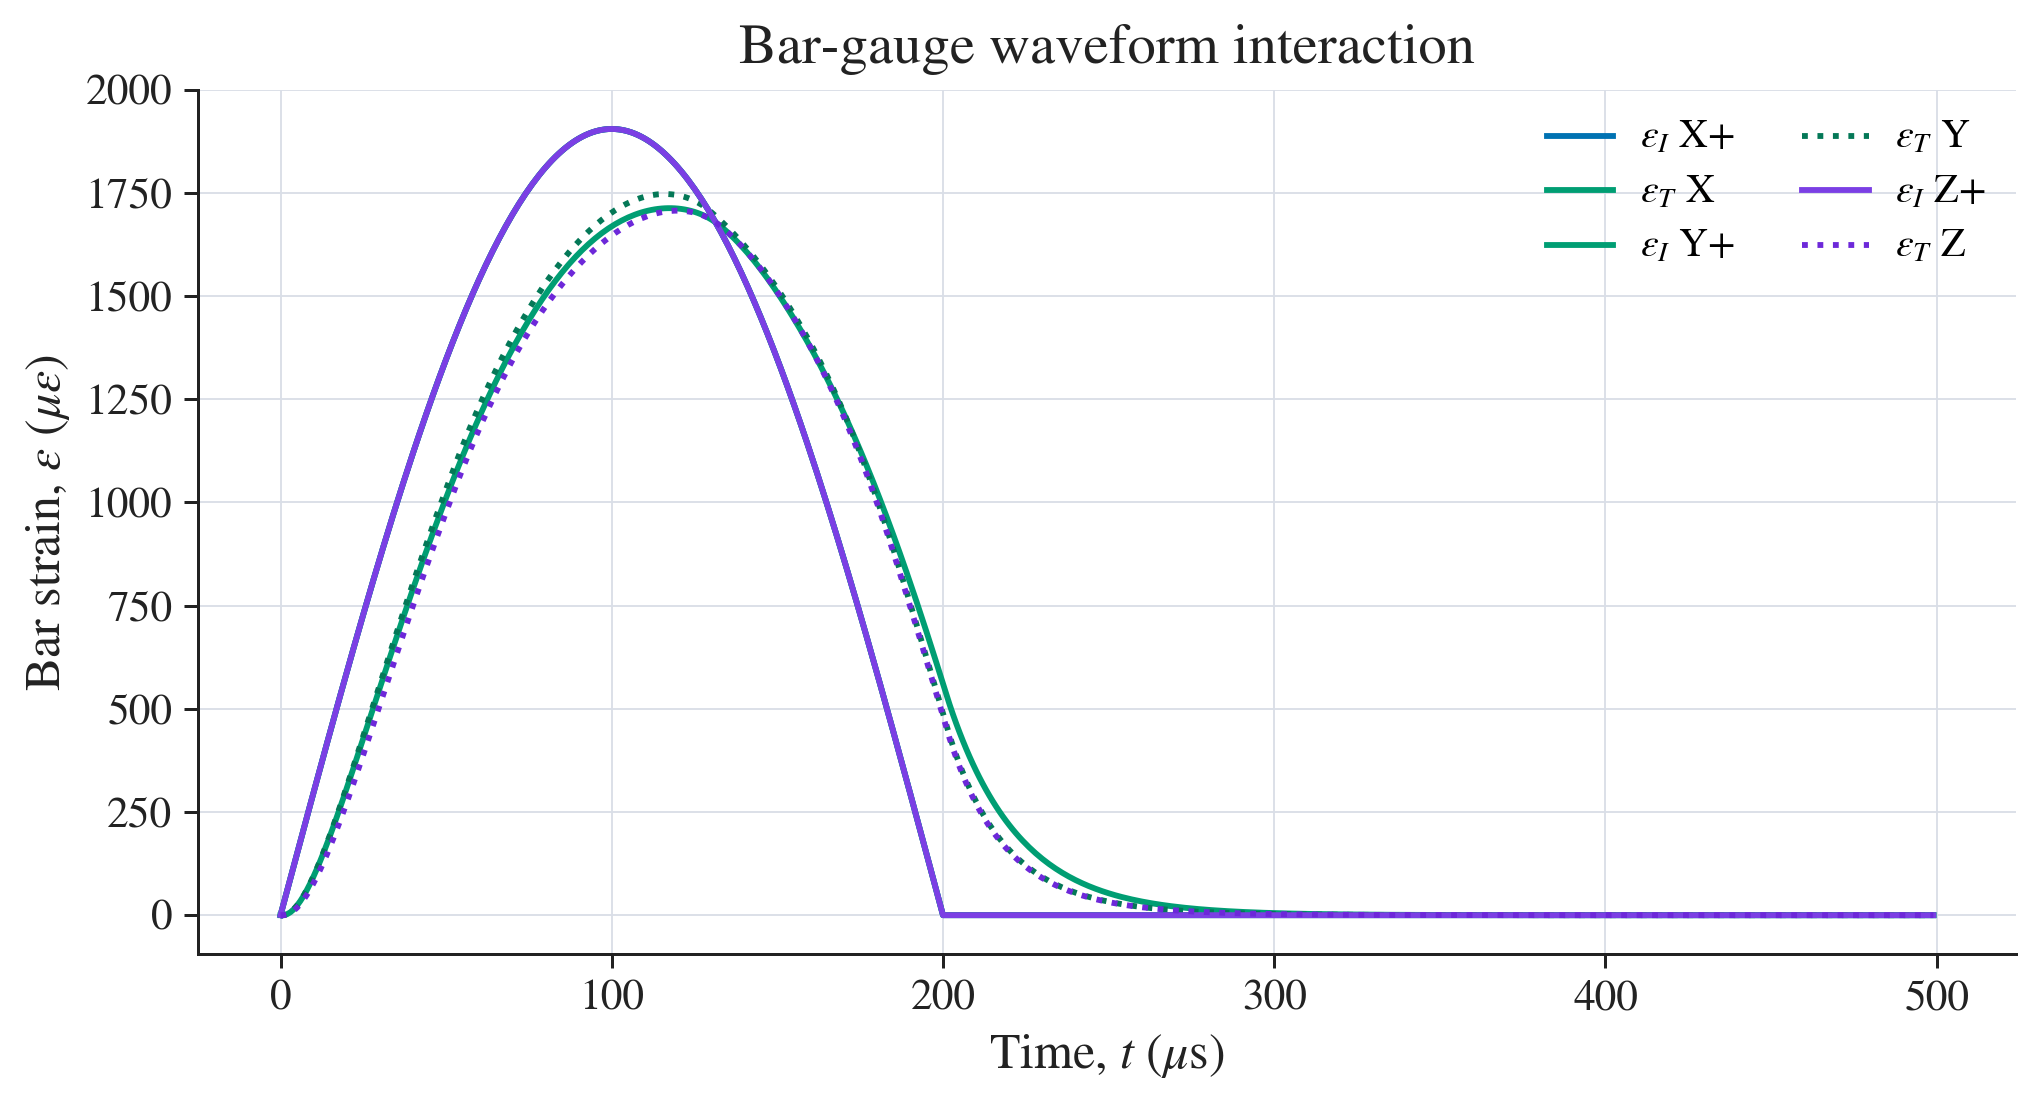
\includegraphics[width=0.92\linewidth]{figures/handbook_modes/mode_5_em_async_triaxial_bar_signals.png}
  \caption{Mode~5 default sandstone case: active X, Y, and Z bar-gauge histories for the multi-axis electromagnetic drive.}
  \label{fig:mode-5-em-async-triaxial-bar-signals}
\end{figure}

\begin{figure}[htbp]
  \centering
  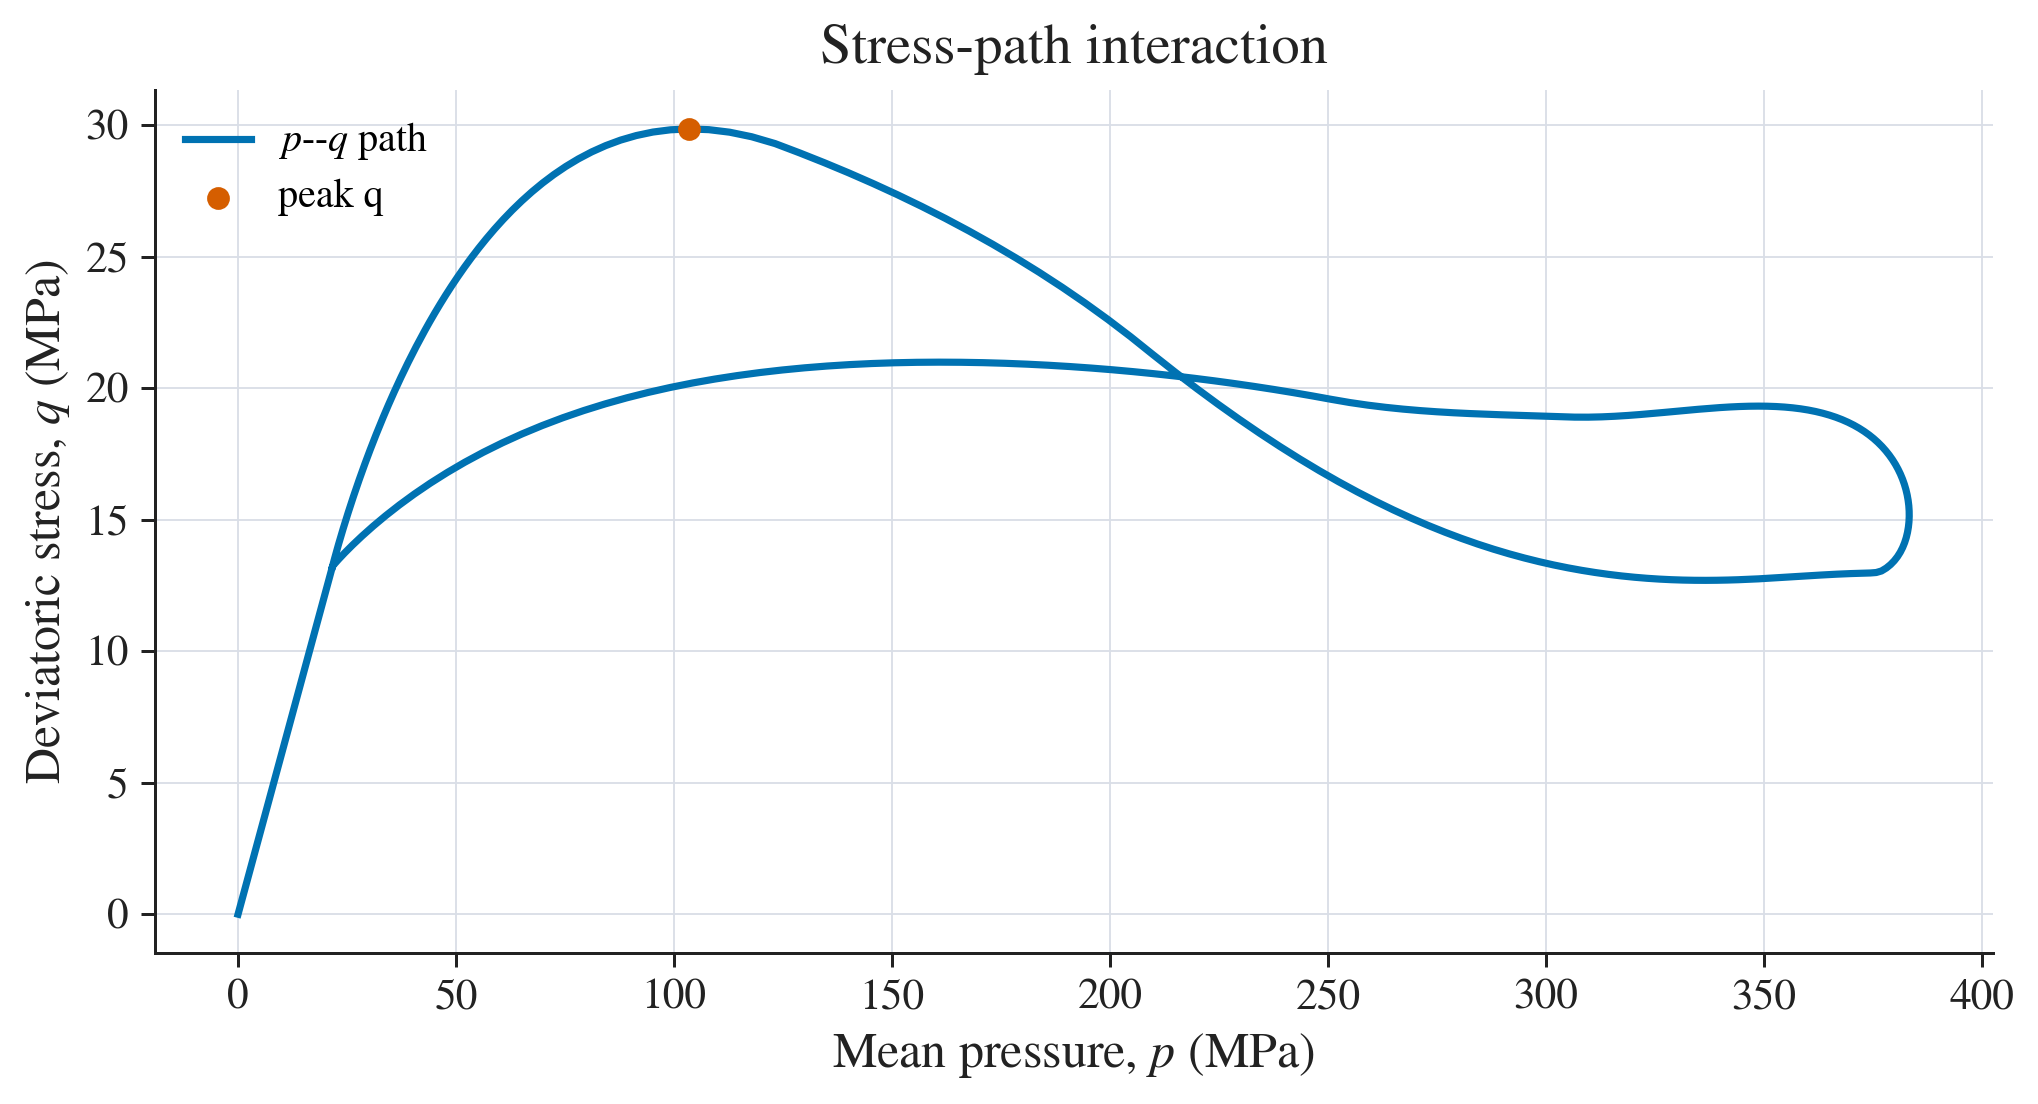
\includegraphics[width=0.92\linewidth]{figures/handbook_modes/mode_5_em_async_triaxial_stress_path.png}
  \caption{Mode~5 default sandstone case: $p$--$q$ projection of the three-axis stress path.}
  \label{fig:mode-5-em-async-triaxial-stress-path}
\end{figure}

\section{Procedure}

\begin{stepbox}[Mode~5 procedure]
\begin{enumerate}[leftmargin=*,itemsep=3pt]
  \item Apply static pre-stress $\sig_1^{0}$, $\sig_2^{0}$, $\sig_3^{0}$.
        Record baselines.
  \item Choose active axes X, X+Y, or X+Y+Z. For any active Y/Z pulse,
        choose delays $\Delta t_y$, $\Delta t_z$ relative to
        $\Delta t_x=0$. Typical values are $\Delta t=0$ (synchronous,
        ground truth), $\Delta t=\tau/4$ (mild asynchrony), and
        $\Delta t=\tau/2$ (strong asynchrony), with the app slider allowing
        values up to \SI{500}{\micro s}.
  \item Set capacitor-bank voltages for the requested per-axis amplitudes
        $A_x$, $A_y$, and $A_z$; equal voltages are a special synchronous
        calibration case rather than a requirement.
  \item Trigger generators with the programmed delays. Synchronisation
        jitter must be much less than $\tau$; aim for $<\SI{1}{\micro s}$
        on a \SI{200}{\micro s} pulse.
  \item Capture each active axis as its own one-sided three-wave record:
        incident, reflected, and transmitted/output histories on X, Y, and
        Z. In the current Streamlit implementation the $-Y$ and $-Z$ bars
        are the transmitted/output bars for their axes; there are no
        additional passive lateral-output gauges beyond those per-axis
        three-wave records.
  \item Subtract baselines, time-align each channel to its own specimen
        face.
  \item Apply the three-wave method on each axis independently.
  \item Plot the principal-stress trajectory
        $(\sig_1(t),\sig_2(t),\sig_3(t))$ in principal-stress space (or use
        the $p$--$q$ projection of Chapter~\ref{ch:wavedamage}).
  \item Compare against a matched synchronous test ($\Delta t=0$) to
        extract the path-dependence effect.
\end{enumerate}
\end{stepbox}

\begin{figure}[htbp]
  \centering
  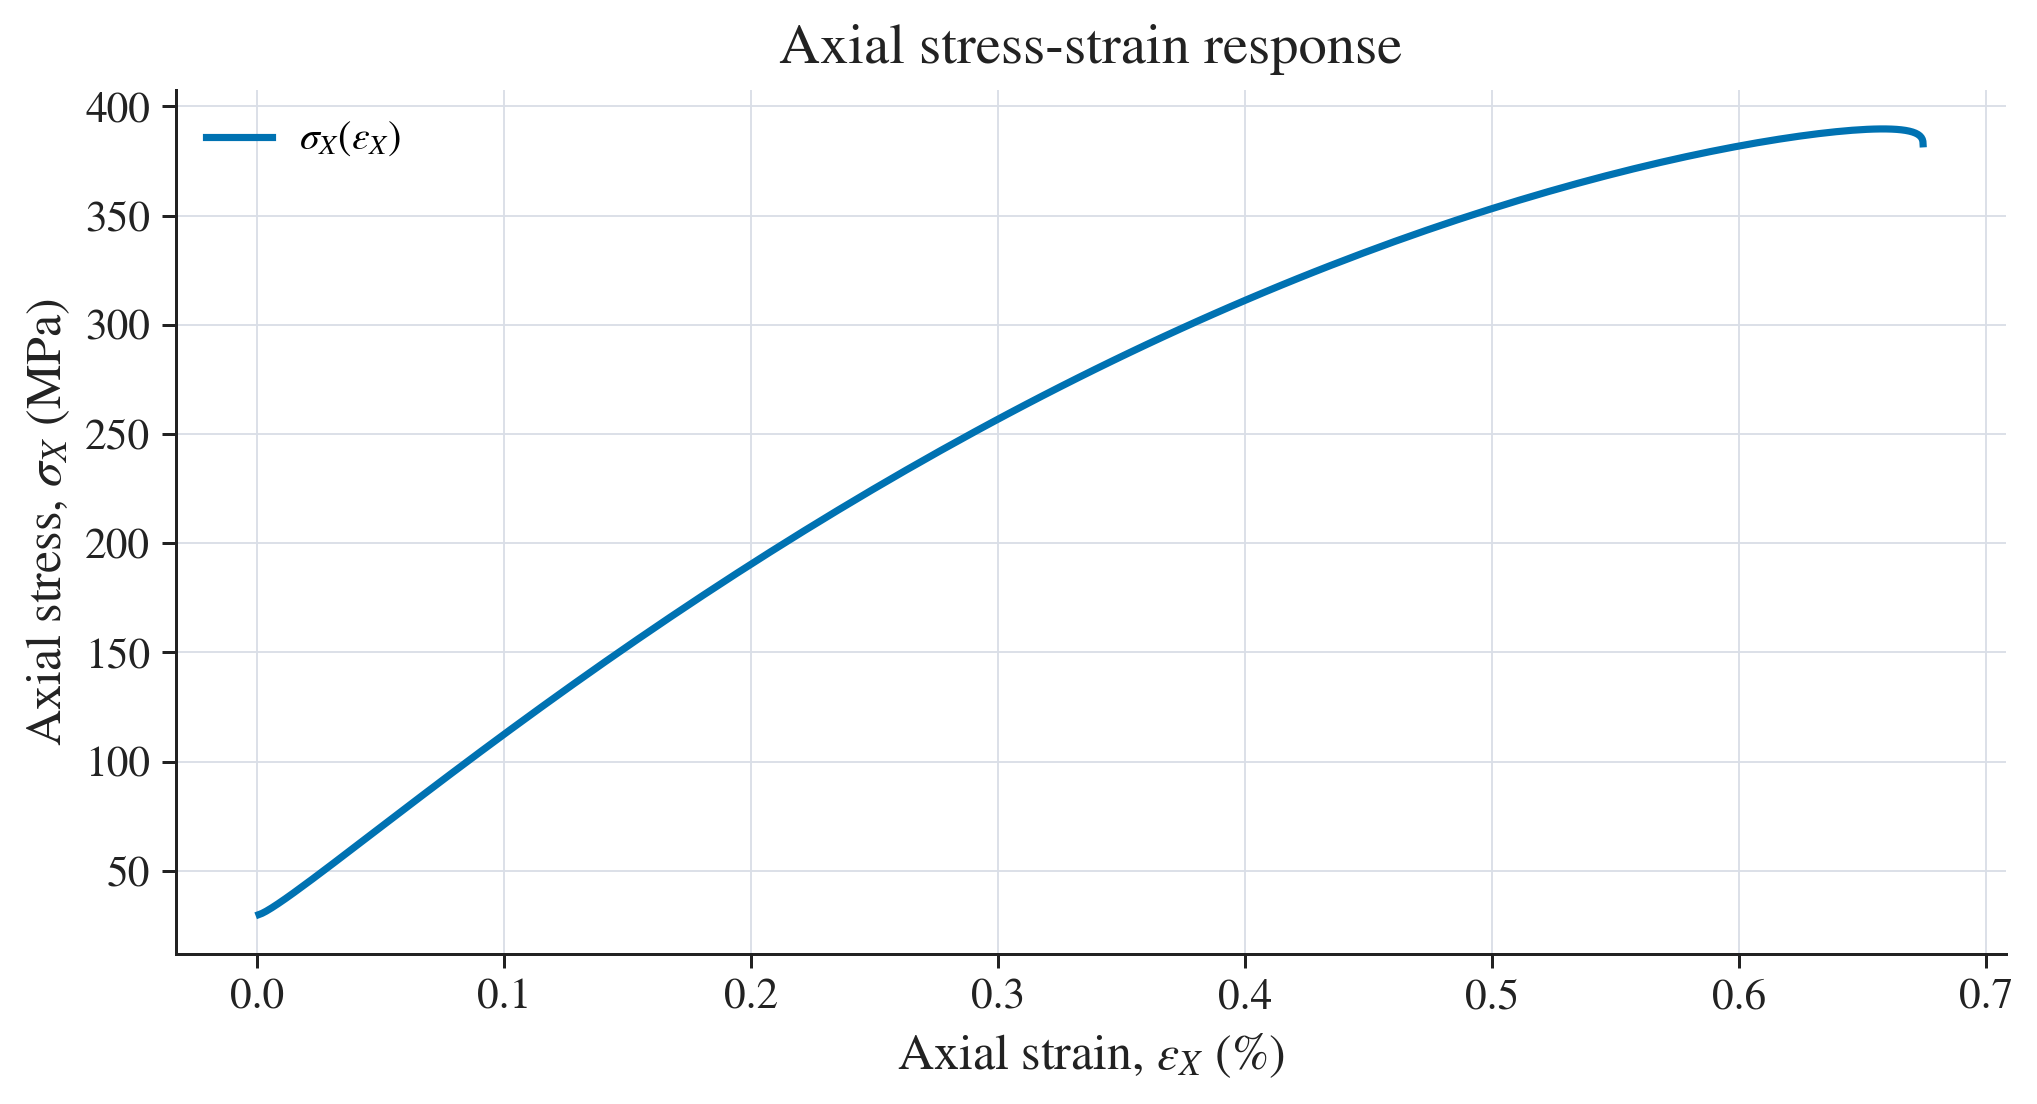
\includegraphics[width=0.92\linewidth]{figures/handbook_modes/mode_5_em_async_triaxial_stress_strain.png}
  \caption{Mode~5 default sandstone case: axial stress--strain branch under three-axis electromagnetic loading.}
  \label{fig:mode-5-em-async-triaxial-stress-strain}
\end{figure}

\section{Validity notes}

\begin{itemize}[leftmargin=*]
  \item All three axes are subject to the same bar plasticity limit. For
        $\sigpeak=\SI{500}{MPa}$ pulses on all three axes, no individual
        bar exceeds \SI{500}{MPa}.
  \item Equilibrium verification is harder in this mode because the
        specimen responds simultaneously to three different loadings.
        Equation \eqref{eq:equilibrium} must be checked \emph{on each axis
        separately}.
  \item The constitutive interpretation requires a full 3D stress-path
        analysis. A uniaxial constitutive model cannot be fitted to data
        from this mode without producing spurious parameters.
\end{itemize}

%==============================================================================
\chapter{Mode 6: Electromagnetic symmetric multidirectional impact}\label{ch:mode6}
%==============================================================================

This is the most powerful and most physically distinctive mode of the Tri-HB
facility. Opposing electromagnetic generators fire \emph{simultaneously} on
each active bar pair. In the full hydrostatic setting this means all six bars
fire as matched pairs $(+X,-X)$, $(+Y,-Y)$, and $(+Z,-Z)$. The two pulses on
each active axis arrive at the specimen at the same instant, superposing
constructively in force while cancelling in momentum.

\begin{newfeature}[Why this mode is special]
\begin{itemize}[leftmargin=*,itemsep=2pt]
  \item Force doubling at each face via constructive superposition.
  \item Zero net momentum transfer --- the specimen does not accelerate.
  \item No transmission bar exists on the active axes; both
        $\pm$-direction bars are incident-only.
  \item Bar stress is unchanged from uniaxial mode at the same $\sigpeak$.
        Doubling occurs in the \emph{specimen} stress, not the bar stress,
        which is a profound advantage for high-stress testing.
  \item Pure hydrostatic loading is possible when all six bars fire equally:
        the deviatoric stress $q\to 0$ and the specimen probes its
        volumetric (cap) response. In the current app this full-XYZ
        topology also links the static pre-stress through one hydrostatic
        slider $p_0=\sig_1=\sig_2=\sig_3$.
\end{itemize}
\end{newfeature}

\section{Symmetry of the wave field}\label{sec:sym-wave-field}

Consider a single axis, say X. In symmetric mode both the $+X$ and $-X$ bars
carry identical incident pulses arriving at the specimen face at the same
instant. Define
\begin{align}
  \eps_{I}^{+}(t) &\;=\; \text{incident wave on the }+X\text{ bar, propagating }-x, \\
  \eps_{I}^{-}(t) &\;=\; \text{incident wave on the }-X\text{ bar, propagating }+x.
\end{align}
By construction, in symmetric mode $\eps_I^{+}=\eps_I^{-}=\eps_I$ at the
specimen position. After interaction with the specimen, each bar carries a
reflected wave $\eps_R^{+}$ or $\eps_R^{-}$ travelling back outward. The
digital twin records both reflected waves explicitly so that the symmetric
energy folding \eqref{eq:sym-energy} can be applied directly.

\begin{figure}[htbp]
  \centering
  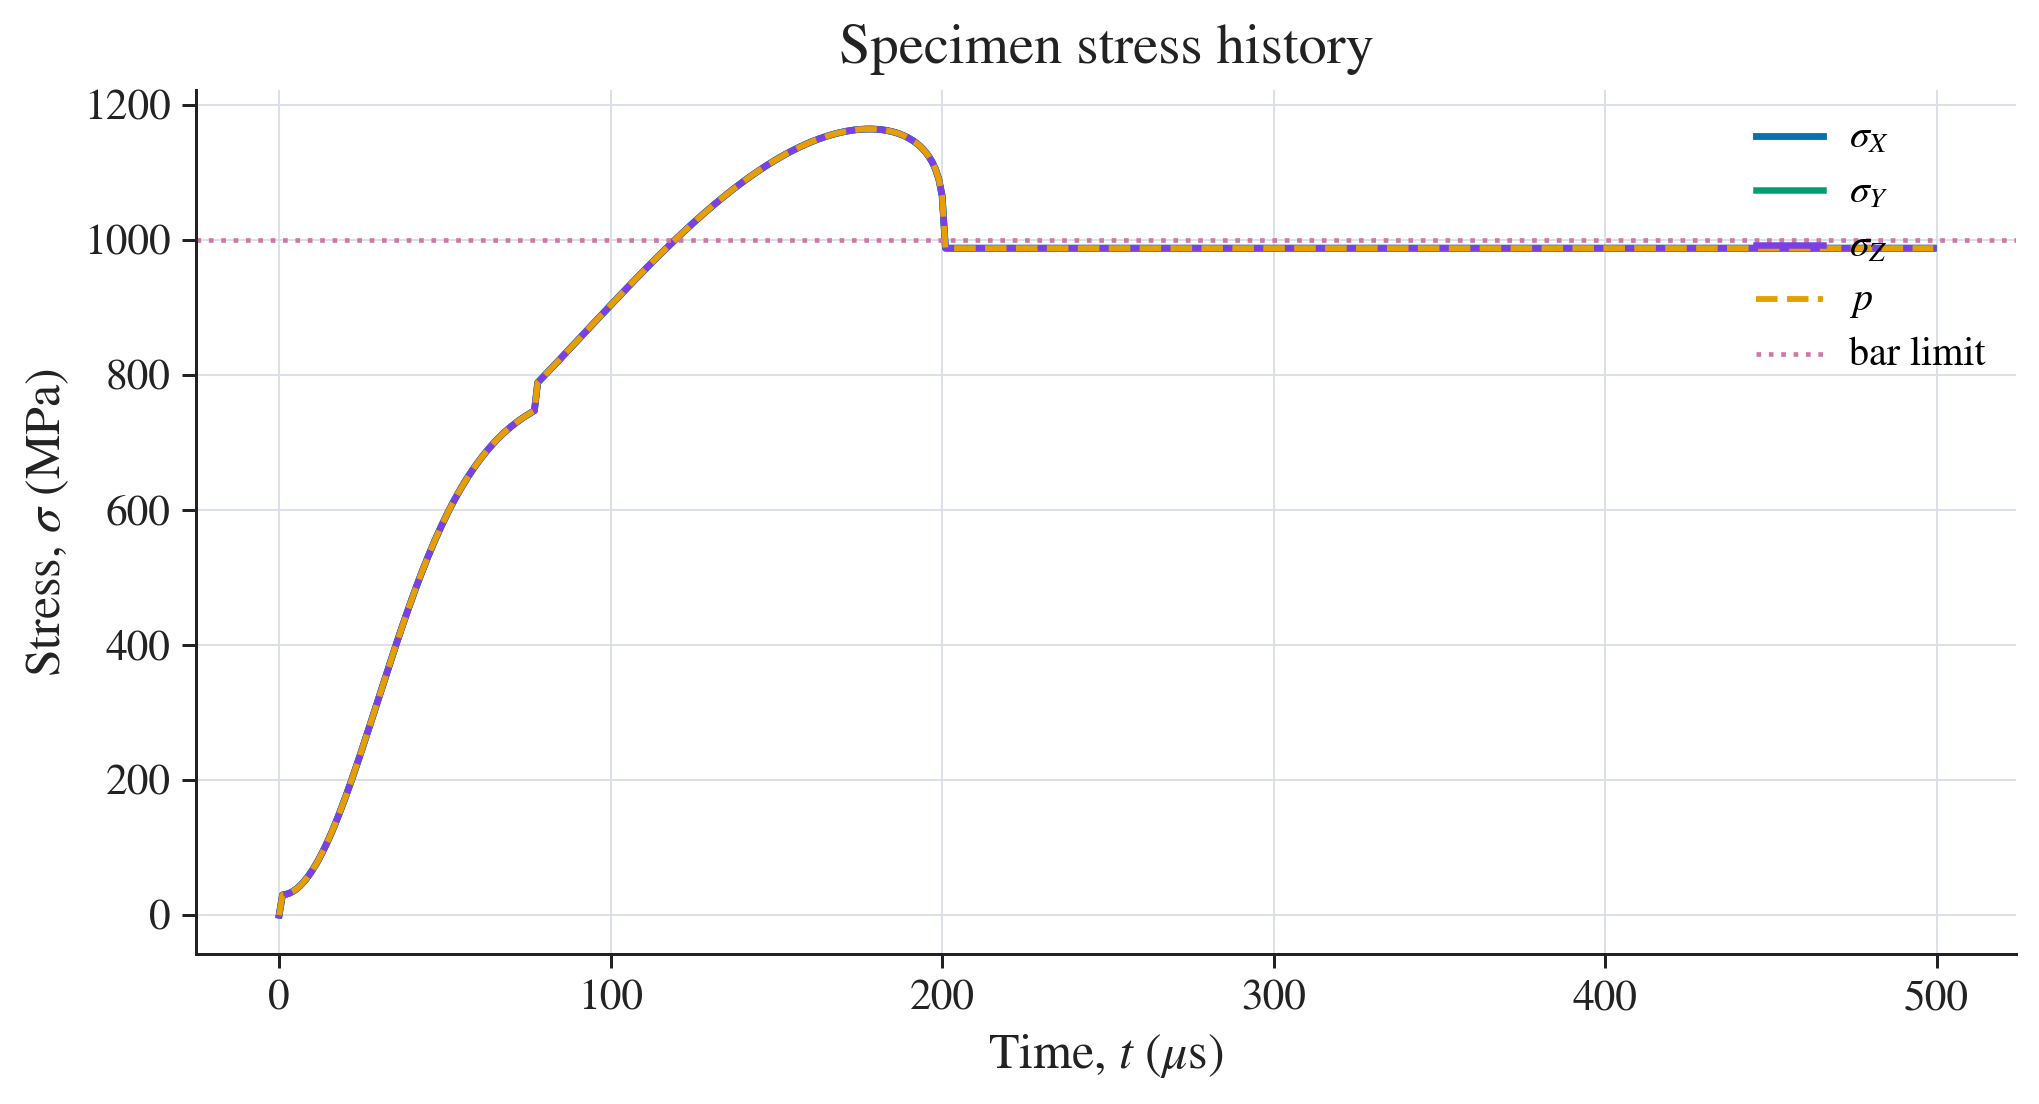
\includegraphics[width=0.92\linewidth]{figures/handbook_modes/mode_6_em_symmetric_xyz_stress_history.png}
  \caption{Mode~6 default sandstone case: total stress history for the full symmetric XYZ electromagnetic configuration.}
  \label{fig:mode-6-em-symmetric-xyz-stress-history}
\end{figure}

\section{Derivation of the symmetric-mode wave equations}

The analogue of the three-wave equations \eqref{eq:sig3wave}--%
\eqref{eq:eps3wave} is derived in four steps.

\subsection*{Step A: Force at the specimen face from each bar}

Each bar end exerts a force on the adjoining specimen face, given by the
boundary-condition relation~\eqref{eq:F1}:
\begin{align}
  F^{+}(t) &\;=\; E_b\Ab\,\bigl[\eps_I^{+}(t) + \eps_R^{+}(t)\bigr],
  \label{eq:Fplus} \\
  F^{-}(t) &\;=\; E_b\Ab\,\bigl[\eps_I^{-}(t) + \eps_R^{-}(t)\bigr].
  \label{eq:Fminus}
\end{align}
Each force acts inward on the specimen.

\subsection*{Step B: Force balance on the specimen}

Dynamic equilibrium of the specimen requires $F^{+}=F^{-}$, otherwise the
specimen would translate as a rigid body. By the symmetry of the input
pulses this condition is automatic. The specimen axial stress is the
force divided by the specimen cross-section:
\begin{empheq}[box=\fbox]{equation}
  \sig_s^{\text{sym}}(t)
    \;=\; \frac{F^{+}+F^{-}}{2\As}
    \;=\; \frac{E_b\Ab}{\As}\,\bigl[\eps_I(t) + \eps_R(t)\bigr],
  \label{eq:sig-sym}
\end{empheq}
where the last equality uses $\eps_I^{+}=\eps_I^{-}=\eps_I$ and
$\eps_R^{+}=\eps_R^{-}=\eps_R$ under perfect symmetry. The prefactor is
$E_b\Ab/\As$, \emph{double} that of the three-wave result
\eqref{eq:sig3wave}, because two bars now drive the specimen instead of
one.

\subsection*{Step C: Velocity of each specimen face}

From \eqref{eq:v1}, the $+X$ bar end velocity is
\[
  v^{+}_{\text{bar}} \;=\; \Cz\,(\eps_I^{+}-\eps_R^{+}) \;=\; \Cz\,(\eps_I-\eps_R),
\]
which is the inward velocity of the $+X$ specimen face. By symmetry the
$-X$ face moves inward at the same rate. The total rate of compression of
the specimen is the sum of the two inward velocities divided by the
specimen length:
\begin{empheq}[box=\fbox]{equation}
  \epsdot_s^{\text{sym}}(t)
    \;=\; \frac{v^{+}+v^{-}}{\Ls}
    \;=\; \frac{2\Cz}{\Ls}\,\bigl[\eps_I(t)-\eps_R(t)\bigr].
  \label{eq:epsdot-sym}
\end{empheq}
The strain rate is doubled relative to one-sided modes at the same
$\sigpeak$. The factor of 2 in \eqref{eq:epsdot-sym} is purely geometric:
both faces move inward, not just one.

\subsubsection*{Numerical note on initial conditions}

In numerical implementation, the simplified driver
$\epsdot_s^{\text{sym}}(t)\approx(2\Cz/\Ls)\eps_I^{+}(t)$ is used to avoid a
spurious deadlock at $t=0$, where the reflected wave momentarily equals
the incident wave before any specimen stress has built up. The simplified
form becomes exact once equilibrium is reached.

\subsection*{Step D: Closure for the reflected wave}

The reflected wave $\eps_R$ is obtained by inverting \eqref{eq:sig-sym}:
\begin{empheq}[box=\fbox]{equation}
  \eps_R(t) \;=\; \frac{\sig_s(t)\,\As}{E_b\Ab} \;-\; \eps_I(t).
  \label{eq:R-sym}
\end{empheq}
This is the analogue of the one-wave reduction $\eps_T = \sig_s\As/(E_b\Ab)$
of the standard analysis (\S\ref{sec:one-wave}); the formula is structurally
identical, with the transmitted wave $\eps_T$ replaced by the reflected wave
$\eps_R$ of the symmetric configuration.

\begin{remark}
An earlier internal draft of this derivation contained an erroneous factor
of 2 in the denominator of \eqref{eq:R-sym}, arising from a
double-counting of the force balance. Equation \eqref{eq:R-sym} as stated
here is consistent with the stress definition \eqref{eq:sig-sym} and has
been validated against the numerical implementation in
\texttt{tri\_hb\_integrated.py}.
\end{remark}

\begin{figure}[htbp]
  \centering
  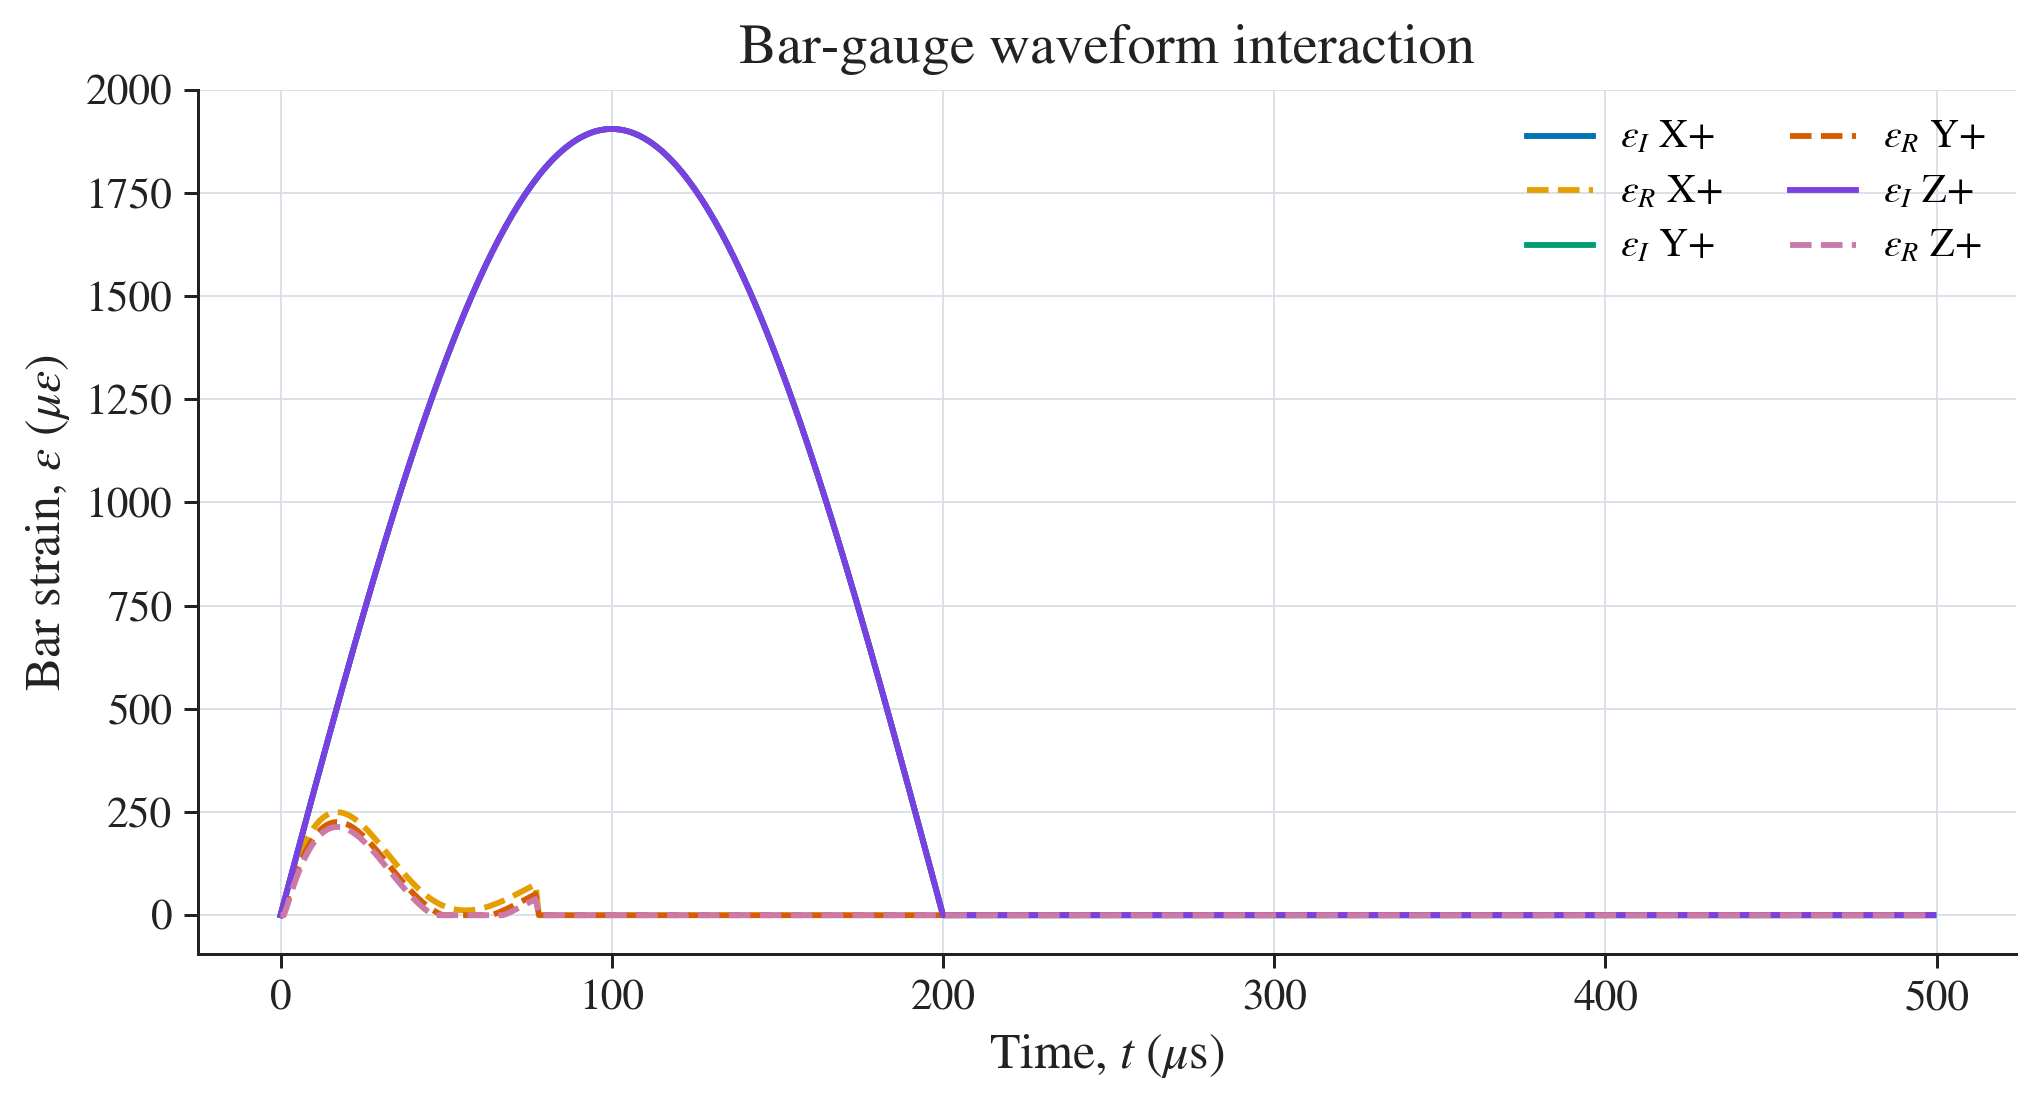
\includegraphics[width=0.92\linewidth]{figures/handbook_modes/mode_6_em_symmetric_xyz_bar_signals.png}
  \caption{Mode~6 default sandstone case: paired incident and reflected bar-gauge histories for symmetric multi-axis loading.}
  \label{fig:mode-6-em-symmetric-xyz-bar-signals}
\end{figure}

\section{Comparison: standard vs symmetric mode}

\begin{center}
\renewcommand{\arraystretch}{1.4}
\begin{tabular}{@{}lcc@{}}
\toprule
\textbf{Quantity} & \textbf{Modes 1--5} & \textbf{Mode 6 (symmetric)}\\
\midrule
Specimen stress
  & $\sig=\dfrac{E_b\Ab}{2\As}(\eps_I+\eps_R+\eps_T)$
  & $\sig=\dfrac{E_b\Ab}{\As}(\eps_I+\eps_R)$\\
Strain rate
  & $\epsdot=\dfrac{\Cz}{\Ls}(\eps_I-\eps_R-\eps_T)$
  & $\epsdot=\dfrac{2\Cz}{\Ls}(\eps_I-\eps_R)$\\
Active bars
  & $\eps_I,\eps_R,\eps_T$ (three)
  & $\eps_I^{\pm},\eps_R^{\pm}$ (two pairs)\\
Ideal paired incident drive
  & $\sig_{\text{drive}}=\sigpeak$
  & $\sig_{\text{drive}}=2\sigpeak$\\
Max bar stress
  & $\sig_{\text{bar}}^{\max}\le\sigpeak$
  & $\sig_{\text{bar}}^{\max}\le\sigpeak$\\
Max specimen $\sig$
  & $\sim\sigpeak$
  & $\sim 2\sigpeak$\\
\bottomrule
\end{tabular}
\end{center}

\begin{warningbox}[The fundamental advantage of symmetric mode]
The bar stress is the \emph{same} in symmetric mode as in uniaxial mode at
the same $\sigpeak$, but the specimen experiences \emph{double} the stress.
Symmetric mode therefore reaches specimen stresses that would require bar
yielding in any one-sided mode. For testing strong rocks under high
confinement, this is the only way to access the high-stress regime without
damaging the bars.
\end{warningbox}

\section{Symmetric sub-modes}

The digital twin offers three configurations:

\begin{description}[leftmargin=2em,style=nextline]
  \item[Symmetric $\pm X$ only]
    Two pulses on $\pm X$; Y and Z bars passive. The specimen experiences
    enhanced uniaxial loading --- doubled stress and doubled strain rate
    --- but no triaxial state. Useful as a baseline against which the
    multi-axis modes are compared.
  \item[Symmetric $\pm X\pm Y$ (biaxial)]
    Four pulses on $\pm X$ and $\pm Y$; Z passive. The specimen experiences
    a true biaxial dynamic squeeze. The deviatoric stress along Z drives
    any shear-related failure.
  \item[Full hydrostatic ($\pm X,\pm Y,\pm Z$)]
    All six pulses fire identically. Under perfect symmetry,
    $\sig_x=\sig_y=\sig_z$ and the deviatoric stress $q=0$; the specimen
    cannot fail by shear yielding. Instead it deforms volumetrically along
    its compaction cap. This probes the pressure--volume response captured
    by the curve $p(\eps_v)$ with $p=\tfrac{1}{3}(\sig_x+\sig_y+\sig_z)$
    and $\eps_v=\eps_x+\eps_y+\eps_z$. The app treats this as the
    hydrostatic topology and therefore exposes one static pre-stress
    control $p_0$ rather than three independent $\sig_1,\sig_2,\sig_3$
    sliders.
\end{description}

\section{Pressure--volume response under hydrostatic loading}

For full hydrostatic loading, the relevant constitutive curve is the
compaction (cap) curve, governed by the bulk modulus $K$ in the elastic
regime and by an eventual cap pressure $p_{\text{cap}}$ at which pore
collapse and grain rearrangement take over \cite{Schofield1980}:
\begin{equation}
  \frac{dp}{d\eps_v} \;=\; K \quad(\text{initial elastic regime}),
  \qquad p\to p_{\text{cap}} \quad(\text{post-cap plateau}).
\end{equation}
In the current Streamlit constitutive surrogate, the cap pressure is
rate-scaled using the same DIF convention as the axial strength model:
\begin{equation}
  p_{\text{cap}} = 4\sig_{c0}\,\text{DIF}, \qquad
  \text{DIF}=1+b_{\text{rate}}\log_{10}
  \!\left(\frac{\max(\epsdot,\epsdot_{\text{ref}})}
  {\epsdot_{\text{ref}}}\right).
\end{equation}
The digital twin automatically switches to this constitutive regime when
the full-hydrostatic sub-mode is selected.

\begin{figure}[htbp]
  \centering
  
\includegraphics[width=0.92\linewidth]{figures/handbook_modes/mode_6_em_symmetric_xyz_stress_path.png}
  \caption{Mode~6 default sandstone case: hydrostatic-compaction diagnostic plotted as mean pressure against volumetric strain.}
  \label{fig:mode-6-em-symmetric-xyz-stress-path}
\end{figure}

\section{Procedure}

\begin{stepbox}[Mode~6 procedure]
\begin{enumerate}[leftmargin=*,itemsep=3pt]
  \item Apply static pre-stress: set one hydrostatic value
        $p_0=\sig_1^{0}=\sig_2^{0}=\sig_3^{0}$ for the full hydrostatic
        sub-mode, or the relevant active-axis values otherwise.
  \item Choose $\sigpeak$ (single-bar peak amplitude). Remember the specimen
        will experience $2\sigpeak$ on each active axis. Verify
        $\sigpeak<\sigprop=\SI{1000}{MPa}$.
  \item Choose $\tau$ for the desired strain rate. Because the symmetric
        strain rate is doubled at the same $\tau$, set
        $\tau\approx 2\tau_{\text{uniaxial}}$ for the same target
        $\epsdot$.
  \item Charge the active capacitor banks to identical voltages.
  \item Synchronise the triggers. Synchronisation jitter must satisfy
        $\Delta t_{\text{jitter}}\ll\tau/10$. Modern trigger electronics
        achieve $<\SI{0.5}{\micro s}$.
  \item Capture all bar gauge signals (four per active axis).
  \item Verify symmetry: $\eps_I^{+}\approx\eps_I^{-}$ and
        $\eps_R^{+}\approx\eps_R^{-}$. Asymmetry indicates synchronisation
        failure or non-uniform specimen damage, and invalidates the
        doubled-stress analysis.
  \item Apply \eqref{eq:sig-sym} and \eqref{eq:epsdot-sym} on each active
        axis.
  \item For the hydrostatic sub-mode, compute $p(t)$, $\eps_v(t)$, and plot
        $p(\eps_v)$.
  \item For the biaxial sub-mode, extract both the active-axis
        $\sig$--$\eps$ curves and the passive-axis Poisson response.
  \item Confirm bar plasticity:
        $\max_i|\sig_{\text{bar},i}(t)|<\sigprop$.
\end{enumerate}
\end{stepbox}

\begin{figure}[htbp]
  \centering
  
\includegraphics[width=0.92\linewidth]{figures/handbook_modes/mode_6_em_symmetric_xyz_stress_strain.png}
  \caption{Mode~6 default sandstone case: axial stress--strain branch under symmetric full-XYZ electromagnetic loading.}
  \label{fig:mode-6-em-symmetric-xyz-stress-strain}
\end{figure}

\section{Worked example: concrete under fully hydrostatic loading}

A concrete specimen (UCS $\sig_{c0}\approx\SI{40}{MPa}$) is to be tested
under fully hydrostatic dynamic loading with target peak pressure
$p_{\text{peak}}=\SI{800}{MPa}$. Static pre-stress
$\sig_1^{0}=\sig_2^{0}=\sig_3^{0}=\SI{50}{MPa}$.

\textbf{Required single-pulse amplitude.} Since the specimen sees
$2\sigpeak$ on each axis, and the loading is hydrostatic so that the mean
pressure equals the axial stress,
\begin{align*}
  p_{\text{peak}} &\;=\; \sig_1^{0} + 2\sigpeak,\\
  \SI{800}{MPa} &\;=\; \SI{50}{MPa} + 2\sigpeak \;\Rightarrow\; \sigpeak=\SI{375}{MPa}.
\end{align*}

\textbf{Bar stress check.} Each bar carries one pulse at $\sigpeak$:
\[
  \sig_{\text{bar}}^{\max}\approx\SI{375}{MPa}<\SI{1000}{MPa}\;\checkmark.
\]
Plenty of margin: this configuration is safe even though the same specimen
pressure would require $\sigpeak\approx\SI{750}{MPa}$ in any one-sided
mode, perilously close to the bar limit.

\textbf{Pulse duration.} For a target $\epsdot\sim\SI{300}{s^{-1}}$ in
symmetric mode, the doubled strain-rate prefactor gives
$\tau\approx 2\Cz\eps_I/(\Ls\,\epsdot_{\text{target}})\sim\SI{200}{\micro s}$.

\textbf{Result.} Charge each of six capacitor banks to deliver
$\sigpeak=\SI{375}{MPa}$, $\tau=\SI{200}{\micro s}$, fire synchronously with
$\sig_1^{0}=\sig_2^{0}=\sig_3^{0}=\SI{50}{MPa}$ pre-applied. Expected
outcome: pure compaction response, no shear failure, bar limits
respected.


%==============================================================================
\chapter{Comparison of the six physics branches}\label{ch:comparison}
%==============================================================================

\section{Side-by-side comparison}

\begin{center}
\renewcommand{\arraystretch}{1.4}
\scriptsize
\begin{tabular}{@{}p{2.5cm}p{1.55cm}p{1.55cm}p{1.55cm}p{1.55cm}p{1.55cm}p{1.55cm}@{}}
\toprule
\textbf{Property} & \textbf{Mode 1} \par Gas-gun & \textbf{Mode 2} \par Conf.\ chamber & \textbf{Mode 3} \par Monash Tri-HB & \textbf{Mode 4} \par EM uniaxial & \textbf{Mode 5} \par EM async & \textbf{Mode 6} \par EM sym.\\
\midrule
Pulse shape & Half-sine (shaped) & Half-sine (shaped) & Half-sine (shaped) & Half-sine & Half-sine $\times 3$ & Half-sine $\times 6$ \\
Pulse source & Striker bar & Striker bar & Striker bar & EM coil & EM coil $\times 3$ & EM coil $\times 6$ \\
Specimen shape & Cylindrical / cubic & Cylindrical & Cubic & Cubic & Cubic & Cubic \\
Active dynamic bars & 1 (X) & 1 (X) & 1 (X) & 1 (X) & 1--3 ($+X/+Y/+Z$) & 2--6 ($\pm$ pairs) \\
Lateral architecture & None & Pressure chamber & 4 output bars & 4 output bars & T/output bars on active axes & Reflected bars on active pairs \\
Confining stress & None & $\sig_2{=}\sig_3{=}p_c$ axisym. & $\sig_2,\sig_3$ indep.\ & $\sig_2,\sig_3$ indep.\ & $\sig_2,\sig_3$ indep.\ & Linked $p_0$ for full XYZ \\
Default $\sig_1,\sig_2,\sig_3$ & 0, 0, 0 & 30, 20, 20 & 30, 20, 15 & 30, 20, 15 & 30, 20, 15 & 30, 30, 30 for full XYZ \\
Pre-stress range & 0--50 MPa axial & 0--50 MPa each & 0--50 MPa each & 0--50 MPa each & 0--50 MPa each & 0--50 MPa each \\
Pulse independence & $\sigpeak{\propto}V$, $\tau{\propto}L$ & $\sigpeak{\propto}V$, $\tau{\propto}L$ & $\sigpeak{\propto}V$, $\tau{\propto}L$ & Indep. & Indep. & Indep. \\
Specimen $\sig_{\max}$ & ${\sim}\sigpeak$ & ${\sim}\sigpeak{+}\sig_1$ & ${\sim}\sigpeak{+}\sig_1$ & ${\sim}\sigpeak$ & ${\sim}\sigpeak$ each axis & ${\sim}2\sigpeak$ each axis \\
Lode angle reach & $\theta=0$ & $\theta=0$ fixed & $\theta\in[0^\circ,60^\circ]$ & $\theta=0$ & $\theta\in[0^\circ,60^\circ]$ & $\theta\in[0^\circ,60^\circ]$ \\
Stress-path control & Uniaxial only & Static triax.\ (axisym.) & Static triax.\ + dyn.\ axial & Uniaxial only & Yes (async) & Hydrostatic / biaxial / uniaxial sym. \\
Pure hydrostatic? & No & No & No & No & Approx.\ if equal and synchronous & Full XYZ only \\
Best application & UCS, baseline SHPB & Standard confined SHPB & In-situ confined rock dyn. & Clean rate-dependence & Path-dependent failure & Cap mechanics, high stress \\
\bottomrule
\end{tabular}
\end{center}

\noindent\textit{Note on slider range.} The \SI{50}{MPa} pre-stress cap
reflects the current digital-twin calibration. The slider maximum is set in
one location (\texttt{max\_conf} in \texttt{tri\_hb\_integrated.py}) and can
be raised when the physical bench is upgraded.

\section{Mode selection: matching the question to the apparatus}

\begin{itemize}[leftmargin=*,itemsep=3pt]
  \item \textbf{Mode 1 (Gas-gun, unconfined)} --- when the research question
        is a baseline uniaxial dynamic strength, or a comparison against
        published classical SHPB data. Reliable and well-understood, but
        limited to a single loading axis with no active confinement.
  \item \textbf{Mode 2 (Confinement-chamber SHPB)} --- when triaxial
        confinement is required but only axisymmetric (Lode angle
        $\theta=0$) stress states are of interest. This is the most
        widely deployed triaxial-SHPB configuration in the dynamic-rock
        and dynamic-concrete literature, well suited to high confining
        pressures and cylindrical specimens. Use this when the research
        plan does not call for independent $\sig_2$ versus $\sig_3$.
  \item \textbf{Mode 3 (Monash Tri-HB)} --- when in-situ stress conditions
        matter and the research requires independently controlled $\sig_2$
        and $\sig_3$, or a non-zero Lode angle: dynamic strength of rocks
        under realistic anisotropic triaxial confinement, blast-induced
        rockburst at depth, or any question where the full triaxial
        stress-path state is part of the physics
        \cite{Liu2019,Zhang2019Tri}.
  \item \textbf{Mode 4 (EM Uniaxial)} --- when rate-dependent constitutive
        behaviour is the primary question. The independent control of
        $\sigpeak$ and $\tau$ permits a controlled sweep of the
        $(\sig,\epsdot)$ plane.
  \item \textbf{Mode 5 (EM Asynchronous)} --- when loading-order effects
        are at issue. Particularly relevant for blast-induced rockburst
        and seismic loading. Pair with the Step~2 regime classifier and
        the Step~3 $p$--$q$--$\theta$ path.
  \item \textbf{Mode 6 (EM Symmetric)} --- when (a) the target specimen
        stress exceeds the bar plasticity limit in any one-sided mode, or
        (b) the research targets the volumetric (cap) response of the
        material, which is inaccessible in any one-sided mode.
\end{itemize}

\section{Common pitfalls and digital-twin diagnostics}

\begin{itemize}[leftmargin=*,itemsep=3pt]
  \item \textbf{Bar plasticity violation.} The three-tier warning system of
        \S\ref{sec:bar-plasticity} catches this in real time. Plan every
        physical test in the digital twin first.
  \item \textbf{Loss of stress equilibrium.} For very brittle specimens or
        very short pulses, the specimen may fail before reverberations
        equilibrate it. Check \eqref{eq:equilibrium}. Step~2 reports the
        equilibrium window $t_{\text{eq}}\in[3,5]\,t_{\text{travel}}$ as a
        shaded band on the time-history plot.
  \item \textbf{Confusing strain rate with total strain.} A short,
        high-amplitude pulse delivers high $\epsdot$ but possibly
        insufficient total strain to fail the specimen. Both metrics must
        be checked in the summary panel.
  \item \textbf{Multi-axis misinterpretation.} A uniaxial constitutive model
        cannot be fitted to data from Mode~5. Use a 3D stress-path-aware
        model (Drucker--Prager with cap, Mohr--Coulomb with non-associated
        flow). The Step~3 $p$--$q$--$\theta$ diagnostics identify the
        path.
  \item \textbf{Symmetric-mode synchronisation failure.} If
        $\eps_I^{+}\neq\eps_I^{-}$, the symmetry assumption is broken and
        the doubled-stress analysis is invalid.
  \item \textbf{Sign-convention mismatch.} The Step~1 reducer assumes the
        textbook convention ($\eps_I>0$, $\eps_R<0$, $\eps_T>0$ for a
        compression test). Use the compression-convention radio button to
        flip data acquired with the opposite polarity; an inverted
        convention typically appears as a negative absorbed energy, which
        the digital twin flags explicitly.
\end{itemize}

%==============================================================================
\chapter{The integrated computational workspace}\label{ch:integrated}
%==============================================================================

The Virtual Tri-HB is delivered as a single integrated Streamlit
application, \texttt{tri\_hb\_integrated.py}, that bundles six analysis
steps under one shared experimental setup. This chapter documents the
launch procedure, the navigation structure, and the export pipeline. The
two chapters that follow document the equations of the experimental
reducer (Chapter~\ref{ch:expdata}) and of the wave/damage/DEM module
(Chapter~\ref{ch:wavedamage}).

\section{Launching the application}

\begin{stepbox}[Local launch]
\begin{enumerate}[leftmargin=*,itemsep=3pt]
  \item Install Python $\ge 3.9$; the current local test environment uses
        Python~3.13.
  \item Open PowerShell or a terminal in the repository folder containing
        \texttt{tri\_hb\_integrated.py}, \texttt{Tri-HB.py},
        \texttt{wave\_damage.py}, and \texttt{requirements.txt}.
  \item Install dependencies on Windows:
        \texttt{py -3.13 -m pip install -r requirements.txt}.
  \item Launch the integrated workspace:
        \texttt{py -3.13 -m streamlit run tri\_hb\_integrated.py --server.port 8501}.
  \item The browser opens at \texttt{http://localhost:8501}. If it does
        not, open the URL manually.
\end{enumerate}
\end{stepbox}

\noindent The integrated file \texttt{tri\_hb\_integrated.py} is the
recommended entry point. It loads \texttt{Tri-HB.py} for the Step~1
configuration/simulator page and \texttt{wave\_damage.py} for the Step~2--4
wave, stress-path, damage, energy, and validation pages; the Step~5 summary,
the Step~6 document generators, and the \emph{Validation \& publication plan}
page are rendered by the integrated file itself. The direct command
\texttt{streamlit run tri\_hb\_integrated.py} is equivalent when the
\texttt{streamlit} executable is already on the system path. On macOS or
Linux, replace \texttt{py -3.13} with the local Python launcher, commonly
\texttt{python} or \texttt{python3}.

For shared use across a class, the repository can be pushed to GitHub and
connected via \texttt{share.streamlit.io}. Students then access the
integrated workspace through a public URL with no local installation.

\section{Top-level navigation}

A single radio in the sidebar selects which page is active. The intent is
to move through them in order, but jumping back is supported because each
step reads the shared
\path{tri_hb_latest_config}/\path{tri_hb_latest_result} entries
from the Streamlit session state.

\begin{description}[leftmargin=2em,style=nextline]
  \item[Overview] Landing page that explains the workflow through a schematic
    flow diagram and an interactive isometric animation of the Monash Tri-HB:
    the striker launches a stress pulse down the X incident bar, which reflects
    and transmits at the cubic specimen while the specimen's Poisson expansion
    drives output waves along the Y and Z bars; a synchronised six-gauge scope
    plays underneath. Use it to confirm the handbook matches the deployed
    application version.
  \item[Step 1: Setup, simulator and data]
    Defines the shared experimental setup (material, specimen, bar,
    loading) and produces either a simulated stress--strain history or a
    reduced stress--strain history from uploaded gauge data. A second
    radio inside the sidebar switches between the simulator
    (Chapters~\ref{ch:mode1}--\ref{ch:mode6}) and the data reducer
    (Chapter~\ref{ch:expdata}).
  \item[Step 2: Wave model]
    Pulse timing, travel time, equilibrium window, and the
    wave-superposition / damage-memory regime classifier. Loads the
    \texttt{wave\_damage.py} module with the ``Wave model'' tab first.
  \item[Step 3: Stress path and analysis]
    $p$--$q$--$\theta$ paths, invariant histories, comparison against the
    reduced experimental data from Step~1. Same module, ``Stress path''
    tab first.
  \item[Step 4: Damage model and DEM validation]
    Damage evolution, stiffness and wave-speed degradation, energy
    balance, DEM/experimental descriptors, parametric study, and export.
    Same module, ``Damage evolution'' tab first. Advanced mode exposes the
    true-triaxial Lode and rate-dependent failure envelope
    (\S\ref{sec:v6-envelope}) and the orthotropic damage tensor
    (\S\ref{sec:v6-orthotropic}); the energy balance is the
    first-law-consistent partition of \S\ref{sec:v6-energy}.
  \item[Step 5: Summary of Results]
    A publication-ready summary that collects every prior step's key figure
    in one view. Each figure is rendered at \SI{600}{dpi}, placed beside a
    short plain-language reading guide and an expandable panel of its
    governing equations, with a per-figure PNG download and a one-click ZIP
    of the whole set plus a metrics table. The page reads the shared session
    state, so it shows results for whichever steps have been run; a readiness
    row at the top indicates whether the Step~1 simulator, optional
    experimental reducer, Steps~2--3 wave/stress module, and Step~4 damage
    module are populated.
  \item[Step 6: Report and Presentation]
    A single page with two tabs --- \emph{Report} and \emph{Presentation} ---
    that each generate a \emph{new} document (LaTeX source plus a compiled
    PDF) from the current run's Steps~1--5. The \emph{Report} tab builds a
    short article-class report (overview, test-configuration table, grouped
    key-results table, the captured figures with their descriptions and
    equations, and a scope note). The \emph{Presentation} tab builds a Beamer
    slide deck styled like the Tri-HB Handbook lecture deck, with a title,
    overview, test-configuration, per-step key-result slides, and one slide
    per captured figure (figure beside its description and governing
    equations). Each tab offers the PDF, the editable \texttt{.tex}, and a
    self-contained ZIP (\texttt{.tex} plus figures). Both reuse the exact
    metrics and \SI{600}{dpi} figures captured on the Step~5 summary page, so
    the documents match what was shown there.
  \item[Validation \& publication plan]
    Renders \texttt{docs/validation\_calibration\_plan.md} live (single source
    of truth): the parameter inventory, the staged calibrate-then-blind-predict
    protocol, the honest novelty assessment, and the anisotropic-damage
    roadmap. A download button exports the Markdown.
\end{description}

\noindent Step~6 (both tabs) requires the Step~5 summary to have been
opened at least once in the session (so the metrics and figures are captured
in session state). PDF compilation uses a local \LaTeX{} engine
(\texttt{xelatex} for the Beamer deck, \texttt{pdflatex} for the report); the
workspace locates the engine even when it is not on the process \texttt{PATH}
and installs missing packages silently. If no \LaTeX{} engine is available,
the \texttt{.tex} source and ZIP bundle are still produced for offline
compilation.

\section{Step 1 sidebar: the two tabs}

Within the Step~1 simulator task, the sidebar is split into two tabs
mirroring the operational separation a real test team uses.

\begin{description}[leftmargin=2em,style=nextline]
  \item[Experimental setup]
    Specimen material (preset plus editable $E$, UCS, $\nu$, $\rho$),
    specimen geometry (cross-section, side/diameter, loading length
    $\Ls$), and bar properties (bar $E_b$, $\Cz$, cross-section).
    Defaults match the 42CrMo square \SI{50}{mm}$\times$\SI{50}{mm}
    bench; every value is editable.
  \item[Test loading]
    Loading family selector, and when the electromagnetic family is active,
    an EM topology selector. The four top-level families are gas-gun
    uniaxial SHPB, confinement-chamber SHPB, gas-gun Tri-HB
    static--dynamic loading, and electromagnetic programmable loading. The
    EM topology then chooses single-axis one-sided, multi-axis one-sided, or
    symmetric opposing pairs. Pulse controls expose striker velocity for the
    gas-gun families, per-axis EM amplitudes and duration for one-sided EM,
    per-bar amplitude and duration for symmetric EM, active axes/pairs, and
    Y/Z asynchronous timing where applicable. In the current app the
    one-sided EM Y/Z delay sliders span \SIrange{0}{500}{\micro s}; ticking
    the synchronous shortcut sets both delays to zero.

    \medskip\noindent
    \textbf{Default pre-stress values} (which the sliders populate when
    the loading family or EM topology is changed):
    \begin{itemize}[leftmargin=1.5em,itemsep=2pt]
      \item Mode~1 (Gas-gun, unconfined):
            $\sig_1=\sig_2=\sig_3=\SI{0}{MPa}$.
      \item Mode~2 (Confinement-chamber SHPB):
            $\sig_1=\SI{30}{MPa}$, $\sig_2=\sig_3=p_c=\SI{20}{MPa}$
            (axisymmetric, so the Y and Z sliders are linked to a
            single $p_c$ control).
      \item Mode~3 (Monash Tri-HB):
            $\sig_1=\SI{30}{MPa}$, $\sig_2=\SI{20}{MPa}$,
            $\sig_3=\SI{15}{MPa}$ (three independent sliders).
      \item EM single-axis and EM multi-axis one-sided (legacy Modes~4--5):
            same independent defaults as Mode~3,
            $\sig_1=\SI{30}{MPa}$, $\sig_2=\SI{20}{MPa}$,
            $\sig_3=\SI{15}{MPa}$.
      \item EM symmetric opposing pairs (legacy Mode~6): the $\pm X$ and
            $\pm X\pm Y$ sub-modes use the active-pair stress controls
            appropriate to the selected dimensionality, while the full
            hydrostatic $\pm X\pm Y\pm Z$ sub-mode exposes one hydrostatic
            pre-stress slider $p_0$ and enforces
            $\sig_1=\sig_2=\sig_3=p_0$.
    \end{itemize}
\end{description}

When Step~1 is configured for ``Experimental data analysis'' instead of
the simulator, the sidebar replaces the test-loading controls with the
data-source selector and column-mapping controls described in
Chapter~\ref{ch:expdata}.

\section{Main panel tabs in the Step~1 simulator}

The main panel updates live as inputs change. Five tabs are available; the
fourth ($p$--$\eps_v$) appears only for the full symmetric
$\pm X\pm Y\pm Z$ hydrostatic EM topology.

\begin{description}[leftmargin=2em,style=nextline]
  \item[Bar waveforms] Time-history of all strain-gauge signals. The
    default view is \emph{raw gauge time}, so the incident, reflected, and
    transmitted/output pulses retain their acquisition-time travel delays
    exactly as a bar-gauge record would. The \emph{aligned reduction time}
    option is the next analysis step: it shifts each wave to a common
    specimen-face time origin for stress and strain reduction. The X-axis
    traces $\eps_I,\eps_R,\eps_T$ are always shown when the loading family
    places dynamic load on X. For Mode~3 (Monash Tri-HB),
    two additional passive lateral output-bar traces are plotted
    alongside the X-axis traces: $\eps_{\text{out}}$ (Y output bar) and
    $\eps_{\text{out}}$ (Z output bar), each representing the averaged
    signal of the two opposing output bars on that axis per
    \eqref{eq:lateral-y}--\eqref{eq:lateral-z}. These lateral traces are
    the experimental record of the specimen's Poisson-coupled lateral
    expansion, and serve as the diagnostic for damage-induced dilation.
    For Mode~2 (Confinement-chamber) the lateral output bars are absent
    and only the X-axis traces appear. For one-sided multi-axis EM, the
    active-axis selector permits X, X+Y, or X+Y+Z, and each active axis is
    displayed as its own $\eps_I,\eps_R,\eps_T$ three-wave record. For
    symmetric opposing pairs, there is no transmission bar on an active
    axis; the plotted incident and reflected $\pm$ traces are used to check
    matched timing and amplitude.
  \item[Specimen stresses] Total $\sig_X,\sig_Y,\sig_Z$ on the specimen.
    In the full symmetric hydrostatic topology the mean pressure $p(t)$ is
    overlaid as a dashed reference. A horizontal dashed line at
    \SI{1000}{MPa} indicates the bar proportional limit.
  \item[$\sig$--$\eps$ curve] Loading branch only. The curve traces from
    the start of the pulse through peak strength and post-peak softening,
    stopping when strain plateaus.
  \item[$p$--$\eps_v$] Visible only for the full symmetric
    $\pm X\pm Y\pm Z$ hydrostatic topology. The compaction curve shows the
    initial bulk-modulus slope followed by the cap plateau.
  \item[Equations] Reference card showing the wave-analysis equations
    used by the active mode, including the standard three-wave method
    and the symmetric-mode variant.
\end{description}

\section{Bar-plasticity warning banner}

Whenever the maximum bar stress approaches the proportional limit, a
coloured warning banner appears at the top of the page:
\begin{itemize}[leftmargin=*,itemsep=2pt]
  \item \textcolor{warnorange}{\textbf{Caution}} (yellow) at
        $0.85\,\sigprop$.
  \item \textcolor{warnorange}{\textbf{Warning}} (orange) at $\sigprop$:
        wave analysis becomes nonlinear; results unreliable.
  \item \textcolor{dangerred}{\textbf{Critical}} (red) at
        $\sig_Y=\SI{1080}{MPa}$: bars deform plastically; the
        configuration must not be run on the physical apparatus.
\end{itemize}
This is the digital twin's primary safety feature. The banner should be
clear (or at most cautionary) before any configuration is considered for
physical testing.

\section{Data export from Step~1}

Four export buttons sit at the bottom of the simulator page. Filenames are
auto-generated from the configuration so that re-running with different
parameters produces uniquely-named files for batch comparison.

\begin{center}
\renewcommand{\arraystretch}{1.4}
\small
\begin{tabular}{@{}p{3.4cm}p{2cm}p{8.5cm}@{}}
\toprule
\textbf{Button} & \textbf{Format} & \textbf{Contents} \\
\midrule
All Signals & CSV &
  Time-series: aligned reduction time, raw gauge/acquisition-time columns
  (\texttt{time\_aligned\_us}, \texttt{time\_gauge\_incident\_us},
  \texttt{time\_gauge\_reflected\_us}, and
  \texttt{time\_gauge\_transmitted\_us} where available), all bar gauge strains
  ($\eps_I^{\pm},\eps_R^{\pm},\eps_T,\eps_Y,\eps_Z$ as available),
  specimen stresses ($\sig_X,\sig_Y,\sig_Z$), strains, pressure,
  volumetric strain, axial strain rate. \\
$\sig$--$\eps$ curve & CSV &
  Loading branch only: axial strain, axial stress, mean pressure,
  volumetric strain. \\
Configuration & JSON &
  Full input configuration, summary metrics, bar/rock properties,
  warning state, time-basis/gauge-location metadata, EM fields
  \texttt{loading\_family}, \texttt{em\_topology}, \texttt{active\_axes},
  \texttt{legacy\_mode}, per-axis amplitudes, and ISO~8601 export
  timestamp. Provides full provenance. \\
Full workbook & XLSX &
  Multi-sheet Excel: Sheet~1 Signals, Sheet~2 Stress-Strain,
  Sheet~3 Configuration. \\
\bottomrule
\end{tabular}
\end{center}

\begin{conceptbox}[Recommended export workflow]
For coursework and research projects:
\begin{enumerate}[leftmargin=2em,itemsep=2pt]
  \item Run the simulator with the chosen configuration.
  \item Verify the bar-plasticity banner is clear.
  \item Export the JSON \emph{and} either the CSV or XLSX, both under the
        auto-generated filename.
  \item Move to Steps 2--4 to interpret wave timing, stress path, and
        damage; these inherit the Step~1 setup through session state.
  \item Export Step~4's CSV for damage and energy histories alongside the
        Step~1 file. The JSON provides the audit trail linking both.
  \item Open Step~5 to capture the publication-quality figure set, then use
        Step~6 (Report and Presentation) to generate ready-to-share
        LaTeX/PDF documents of the run.
\end{enumerate}
\end{conceptbox}

\section{Worked Streamlit session}

\begin{stepbox}[Session: granite at high confinement, EM symmetric XYZ]
\begin{enumerate}[leftmargin=*,itemsep=3pt]
  \item Top sidebar: select \emph{Step 1: Setup, simulator and data}; keep
        the inner radio on \emph{Test design and simulator}.
  \item \emph{Experimental setup} tab: \emph{Material preset = granite},
        keep auto-filled $E$, UCS, $\nu$. Specimen cross-section
        \emph{Square/cube}, side \SI{50}{mm}, $\Ls=\SI{50}{mm}$. Leave bar
        settings at default.
  \item \emph{Test loading} tab: set \emph{Loading family =
        Electromagnetic programmable loading}; set \emph{EM topology =
        Symmetric opposing pairs}; pick \emph{Full hydrostatic
        ($\pm X\pm Y\pm Z$)}.
  \item Per-bar pulse amplitude $A=\SI{400}{MPa}$,
        $\tau=\SI{200}{\micro s}$, and hydrostatic static pre-stress
        $p_0=\sig_1=\sig_2=\sig_3=\SI{50}{MPa}$.
  \item Inspect the warning banner. If it shows ``Caution'' or above,
        reduce $\sigpeak$ until the banner is clear.
  \item Open the $p$--$\eps_v$ tab. Read the slope at low $\eps_v$ (dynamic
        bulk modulus $K_d$) and the plateau at high $\eps_v$ (cap
        pressure).
  \item Click \emph{Full workbook (XLSX)}; verify the
        \emph{Configuration} sheet records all inputs.
  \item Step 2: confirm the equilibrium band; check $\Delta t^{\ast}$
        (should be 0 for a synchronous test).
  \item Step 3: verify the $p$--$q$ path collapses onto the $q\approx 0$
        axis (hydrostatic).
  \item Step 4: read the final damage $D$, central damage fraction $D_c$,
        and energy descriptors. Export the CSV for downstream comparison
        with DEM or experimental data.
  \item Step 5: open \emph{Summary of Results} to capture every step's key
        figure (\SI{600}{dpi}) and the combined metrics table; download the
        per-figure PNGs or the one-click ZIP. Opening this page also captures
        the metrics and figures that Step~6 reuses.
  \item Step 6: open \emph{Report and Presentation}. The \emph{Report} tab
        generates the short run report and the \emph{Presentation} tab the
        Beamer deck; download the compiled PDF, the editable \texttt{.tex}, or
        the ZIP bundle from either tab.
\end{enumerate}
\end{stepbox}

%==============================================================================
\chapter{Experimental data analysis and reduction}\label{ch:expdata}
%==============================================================================

When the inner Step~1 radio is set to ``Experimental data analysis'', the
simulator's loading controls are replaced by a data reducer that converts
raw bar-gauge or direct stress--strain data into the same set of outputs
the simulator produces. Students can therefore compare a real measurement
and a simulation on the same axes, using the same downstream pages (Steps
2--4).

\section{Three data sources}

\begin{description}[leftmargin=2em,style=nextline]
  \item[Latest simulator result]
    Reuses the most recent simulator output stored in session state.
    Useful for verifying agreement between the reducer and the simulator,
    and for feeding simulated data into the energy balance, wave model,
    and damage page.
  \item[Upload bar strain gauges]
    A CSV/XLSX with columns for time and the incident, reflected, and
    transmitted bar strains. The student maps each column manually and
    picks the strain unit (microstrain or strain), the time unit
    (microseconds, ms, or s), and the compression convention (positive or
    negative). The reducer then applies the SHPB equations and produces
    stress, strain, strain rate, and energy histories.
  \item[Upload direct stress--strain]
    A CSV/XLSX already containing a reduced stress and strain. Only unit
    conversion and a numerical derivative for the strain rate are
    needed.
\end{description}

\section{Equations used by the reducer}

Let $E_b$ be the bar Young's modulus, $\Cz=\sqrt{E_b/\rho_b}$ the bar
wave speed, $\Ab$ the bar cross-section, $\As$ and $\Ls$ the specimen
area and length, and $\eps_I,\eps_R,\eps_T$ the incident, reflected, and
transmitted bar strains.

\subsection*{Specimen stress: three-wave average}
\begin{equation}
  \sig_s(t) \;=\; \frac{E_b\Ab}{2\As}\,\bigl[\eps_I(t)+\eps_R(t)+\eps_T(t)\bigr].
  \label{eq:red-3wave}
\end{equation}

\subsection*{Specimen stress: transmitted-wave only}
Assumes force equilibrium $\eps_I+\eps_R\approx\eps_T$:
\begin{equation}
  \sig_s(t) \;=\; \frac{E_b\Ab}{\As}\,\eps_T(t).
  \label{eq:red-1wave}
\end{equation}

\subsection*{Specimen strain rate and strain}
\begin{align}
  \epsdot_s(t) &\;=\; \frac{\Cz}{\Ls}\,\bigl[\eps_I(t)-\eps_R(t)-\eps_T(t)\bigr],\\
  \eps_s(t) &\;=\; \int_{0}^{t}\!\epsdot_s(\tau)\,d\tau \quad (\text{trapezoidal}).
\end{align}
Under perfect equilibrium the rate reduces to $\epsdot_s=-2\Cz\eps_R/\Ls$;
the reducer retains the general three-wave form so that pre-equilibrium
signals are still handled correctly.

\subsection*{Bar-wave energies}
\begin{align}
  W_I(t) &\;=\; E_b\Ab\Cz\!\int_{0}^{t}\!\eps_I^{2}\,d\tau, \\
  W_R(t) &\;=\; E_b\Ab\Cz\!\int_{0}^{t}\!\eps_R^{2}\,d\tau, \\
  W_T(t) &\;=\; E_b\Ab\Cz\!\int_{0}^{t}\!\eps_T^{2}\,d\tau, \\
  W_{\text{abs}}(t) &\;=\; W_I(t) - W_R(t) - W_T(t).
\end{align}
The dimensional check is
$\Ab\,[\si{m^{2}}]\cdot E_b\,[\si{Pa}]\cdot \Cz\,[\si{m/s}]
\cdot\int\eps^{2}\,dt\,[\si{s}] = \si{J}$.

\subsection*{Symmetric-mode (Mode 6) energy folding}
Opposing bar pairs contribute incident \emph{and} reflected pulses
explicitly:
\begin{equation}
  W_I \;=\; E_b\Ab\Cz\!\int\bigl(\eps_{I,+}^{2}+\eps_{I,-}^{2}\bigr)dt,
  \quad
  W_R \;=\; E_b\Ab\Cz\!\int\bigl(\eps_{R,+}^{2}+\eps_{R,-}^{2}\bigr)dt.
\end{equation}

\subsection*{Absorbed energy from simulator stress--strain}
\begin{equation}
  W_{\text{abs}}(t) \;=\; \int_{0}^{t}\!\sig_s(\tau)\,\epsdot_s(\tau)\,V_s\,d\tau,
  \qquad V_s=\As\Ls.
\end{equation}
Because the simulator stores $\sig_s$ as the \emph{total} axial stress
(static pre-load plus dynamic), the reflected, transmitted, and absorbed
energies for a simulator-derived history are computed against the
available incident energy. This monotone closure prevents the
static-preload contribution from appearing as spurious wave energy and
keeps the cumulative budget consistent with the incident envelope.

\subsection*{Direct stress--strain branch}
Only unit conversion and a derivative are required:
\begin{equation}
  \epsdot_s(t) \;=\; \frac{d\eps_s}{dt} \quad (\text{central difference}).
\end{equation}
Strain-unit options: strain (1), percent ($\div 100$), microstrain
($\times 10^{-6}$). Stress-unit options: MPa (pass-through), Pa
($\div 10^{6}$). The compression-convention selector applies a single
global sign so that the formulas above remain consistent with the
textbook convention $\eps_I>0$, $\eps_R<0$, $\eps_T>0$ for a
compression test.

\section{Reducer outputs and energy sanity check}

The reducer writes its output to session state as
\texttt{tri\_hb\_reduced\_data} so that Steps 2--4 can use it for
validation overlays. Outputs include time, stress, strain, strain rate,
and (for bar-gauge data) the four energy histories.

A built-in energy sanity check raises a warning whenever any of
\begin{equation}
  W_T > W_I, \qquad W_R > W_I, \qquad W_{\text{abs}}=W_I-W_R-W_T < 0
\end{equation}
holds. The most common cause is a sign or unit mismatch in the uploaded
file (microstrain reported as strain; mixed compression-positive and
compression-negative columns). The warning reports the numerical excess
so that the student can judge how serious the mismatch is.

\section{Worked reducer session}

\begin{stepbox}[Session: comparing a measurement against the simulator]
\begin{enumerate}[leftmargin=*,itemsep=3pt]
  \item In Step~1, configure and run the simulator to match the geometry
        and loading of the physical test. Note the simulator's peak
        stress and strain rate.
  \item Switch the inner Step~1 radio to ``Experimental data analysis''.
  \item Sidebar: \emph{Data source = Upload bar strain gauges}. The bar
        and specimen geometry inputs inherit the simulator setup
        automatically; override only if the upload was taken with a
        different rig.
  \item Upload the CSV/XLSX. Map the time column and the three strain
        columns. Pick the time and strain units; check the compression
        convention against the raw data (textbook: $\eps_I>0$ for
        compression).
  \item \emph{Stress reduction = Three-wave average} for the baseline;
        then switch to \emph{Transmitted-wave only} to confirm that the
        two formulas agree once equilibrium is reached.
  \item Read the four metric cards: peak stress, peak strain, peak strain
        rate, absorbed energy. Inspect the time-history and energy tabs;
        if the energy warning appears, fix the sign or unit before
        continuing.
  \item Move to Step~3. The ``DEM/experimental descriptors'' overlay (in
        Step~4) will use this reduced dataset for validation comparisons.
\end{enumerate}
\end{stepbox}

%==============================================================================
\chapter{Wave model, stress path, damage and DEM validation}\label{ch:wavedamage}
%==============================================================================

Steps 2, 3, and 4 are three views into a single underlying module
(\texttt{wave\_damage.py}). They share the experimental setup defined in
Step~1 --- material, specimen length, pre-stress, pulse amplitude, pulse
duration, loading dimensionality, asynchronous delay --- and differ only
in which analysis tab is opened first. The equations below are listed once
and apply across all three steps.

\section{Wave-model equations (Step 2 tab)}\label{sec:wave-regime}

\subsection{Elastic constants and wave speeds}

Recalling \eqref{eq:M-lambda}--\eqref{eq:cp-cs}, the constrained modulus
and P-, S-wave speeds are
\begin{align}
  M &\;=\; \frac{E(1-\nu)}{(1+\nu)(1-2\nu)}, \\
  c_p &\;=\; \sqrt{\frac{M}{\rho}},
  \qquad c_s \;=\; \sqrt{\frac{G}{\rho}}.
\end{align}
The wave travel time and the equilibrium window are
\begin{equation}
  t_{\text{travel}} \;=\; \frac{\Ls}{c_p},
  \qquad
  t_{\text{eq}} \;\in\; [3,\,5]\,t_{\text{travel}},
\end{equation}
the latter shaded on the time-history plot.

\subsection{Normalised delay and regime classifier}

\begin{equation}
  \Delta t^{\ast} \;=\; \frac{\Delta t}{t_{\text{travel}}}.
\end{equation}
The digital twin partitions $\Delta t^{\ast}$ into four physically
distinct regimes:
\begin{center}
\renewcommand{\arraystretch}{1.25}
\begin{tabular}{@{}lll@{}}
\toprule
$\Delta t^{\ast}$ & Regime & Dominant physics \\
\midrule
$< 1$ & Synchronous wave superposition & Constructive overlap at specimen \\
$1$ to $3$ & Reverberation-coupled & Internal echoes still strong \\
$3$ to $10$ & Transitional & Decaying reverberations \\
$> 10$ & Sequential, damage-memory & Each pulse acts on a damaged state \\
\bottomrule
\end{tabular}
\end{center}

\subsection{Superposition factor at the specimen centre}

For a pulse envelope $g(\cdot)$ propagating from each end of the specimen,
with right-bar amplitude ratio $r$,
\begin{equation}
  \sig_{\text{centre}}(t) \;=\; \sig_{x0}
     + A_x\,g\!\left(t-\frac{\Ls}{2c_p}\right)
     + A_x\,r\,g\!\left(t-\Delta t-\frac{\Ls}{2c_p}\right),
\end{equation}
\begin{equation}
  \eta_{\text{sup}} \;=\; \frac{\max_t\sig_{\text{centre}}(t)-\sig_{x0}}{A_x}.
\end{equation}
A value $\eta_{\text{sup}}\to 2$ indicates full constructive overlap;
$\eta_{\text{sup}}\to 1$ indicates sequential pulses.

\begin{figure}[htbp]
  \centering
  
\includegraphics[width=0.92\linewidth]{figures/handbook_steps/step2_input_dynamic_pulses.png}
  \caption{Step~2 default sandstone asynchronous XYZ case: input dynamic pulses on the X, Y, and Z loading axes, including the equilibrium-time reference band and inter-axis delays.}
  \label{fig:step2-input-dynamic-pulses}
\end{figure}

\begin{figure}[htbp]
  \centering
  
\includegraphics[width=0.92\linewidth]{figures/handbook_steps/step2_centre_superposition.png}
  \caption{Step~2 default sandstone asynchronous XYZ case: specimen-centre stress indicator used to compute the superposition factor $\eta_{\text{sup}}$.}
  \label{fig:step2-centre-superposition}
\end{figure}

\begin{figure}[htbp]
  \centering
  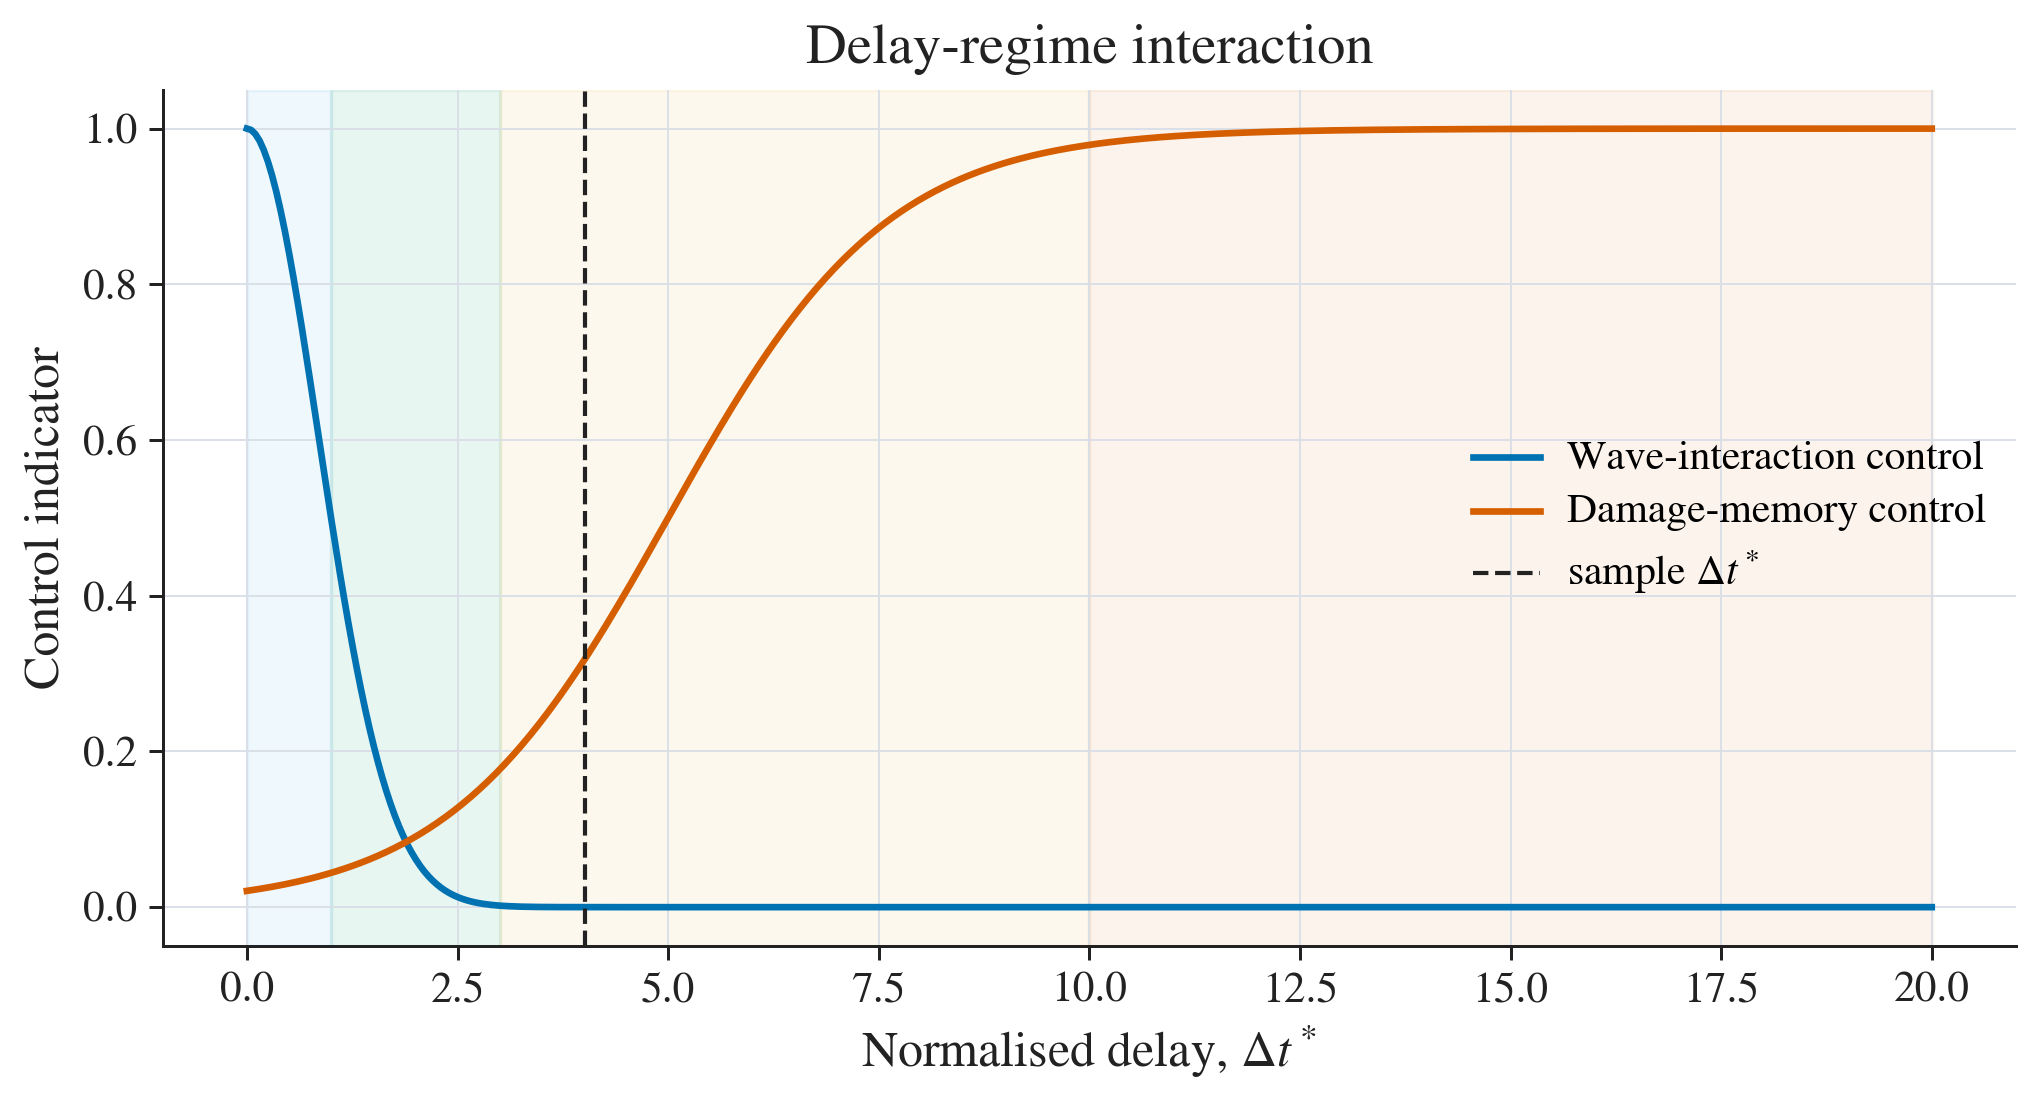
\includegraphics[width=0.92\linewidth]{figures/handbook_steps/step2_delay_regime_map.png}
  \caption{Step~2 default sandstone asynchronous XYZ case: normalised delay regime map separating wave-interaction control from damage-memory control.}
  \label{fig:step2-delay-regime-map}
\end{figure}

\begin{figure}[htbp]
  \centering
  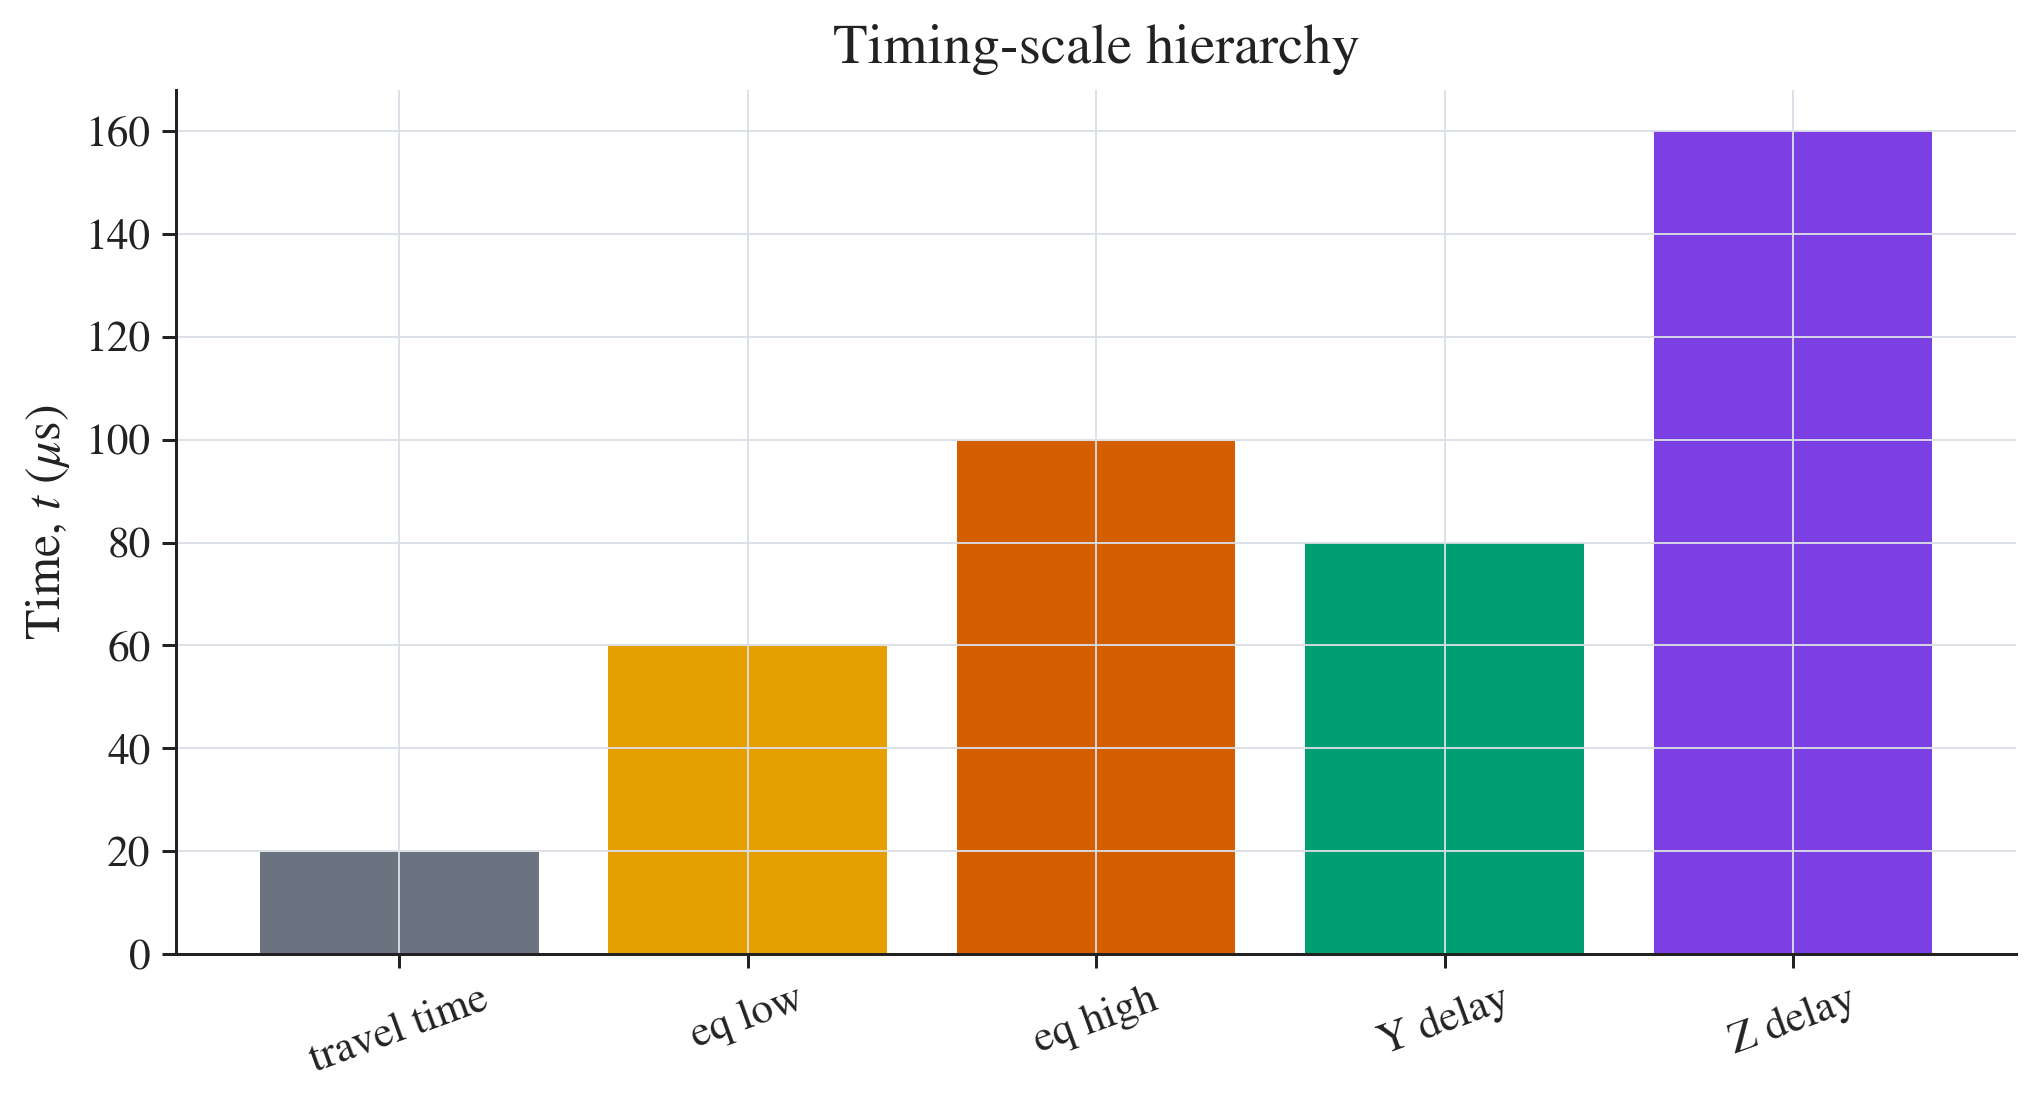
\includegraphics[width=0.92\linewidth]{figures/handbook_steps/step2_timing_scales.png}
  \caption{Step~2 default sandstone asynchronous XYZ case: travel time, equilibrium window, and Y/Z pulse-delay scales used by the workflow.}
  \label{fig:step2-timing-scales}
\end{figure}

\section{Stress-path equations (Step 3 tab)}

Assuming the principal axes align with the bar axes, the diagonal Cauchy
tensor has invariants
\begin{align}
  p   &\;=\; \tfrac{1}{3}(\sig_x+\sig_y+\sig_z), \\
  q   &\;=\; \sqrt{\tfrac{1}{2}\bigl[(\sig_x-\sig_y)^{2}+(\sig_y-\sig_z)^{2}+(\sig_z-\sig_x)^{2}\bigr]}, \\
  J_2 &\;=\; \tfrac{1}{2}(s_1^{2}+s_2^{2}+s_3^{2}), \quad s_i=\sig_i-p, \\
  J_3 &\;=\; s_1 s_2 s_3, \\
  \cos(3\theta) &\;=\; \frac{3\sqrt{3}}{2}\,\frac{J_3}{J_2^{3/2}}.
\end{align}
The Lode angle $\theta$ distinguishes triaxial compression ($\theta=0$)
from triaxial extension ($\theta=60^{\circ}$) and from pure shear
($\theta=30^{\circ}$).

\subsection{Failure surface and failure index}

The failure surface is taken in the pressure- and Lode-angle-dependent form
\begin{align}
  h(\theta) &\;=\; 1 + a_\theta\bigl(1-\cos 3\theta\bigr), \\
  q_f(p,\theta) &\;=\; \bigl(A + B\,p^{n}\bigr)\,h(\theta), \\
  F(t) &\;=\; \frac{q(t)}{q_f(t)}.
\end{align}
The failure index $F$ is dimensionless; $F>1$ means the stress state lies
outside the failure surface and damage is allowed to grow.

\paragraph{Consistency with the Step-1 strength.} To keep the Step-3 failure
index consistent with the Step-1 axial strength
$\sig_1^{\text{peak}}=(\sig_{c0}+k_{\text{conf}}\sig_{\text{conf}})\,\text{DIF}$,
the surface constants are \emph{derived} from the same strength model rather
than set independently. For triaxial compression ($\theta=0$, $h=1$,
$\sig_2=\sig_3=\sig_{\text{conf}}$) one has $q=\sig_1-\sig_{\text{conf}}$ and
$p=(\sig_1+2\sig_{\text{conf}})/3$; eliminating $\sig_{\text{conf}}$ gives the
linear Mohr--Coulomb form
\begin{equation}
  q_f \;=\; A + B\,p, \qquad
  A=\frac{3\,\text{UCS}_{\text{eff}}}{k_{\text{conf}}+2}, \quad
  B=\frac{3\,(k_{\text{conf}}-1)}{k_{\text{conf}}+2}, \quad n=1,
  \label{eq:qf-derived}
\end{equation}
with $\text{UCS}_{\text{eff}}=\text{UCS}\cdot\text{DIF}$. This reproduces the
Step-1 failure point exactly ($F=1$ at peak) for every preset and confinement.
The integrated workspace computes \eqref{eq:qf-derived} automatically from the
Step-1 material; Advanced mode allows $A,B,n,a_\theta$ to be overridden with
independently calibrated values when fitting true-triaxial data.

\subsection{Equivalent (deviatoric) strain rate}

Using elastic strains $\eps_i=\sig_i/E$ as a planning-grade estimate,
\begin{equation}
  \epsdot_{\text{eq}} \;=\;
  \sqrt{\tfrac{2}{3}\cdot\tfrac{1}{2}
        \bigl[(\epsdot_x-\epsdot_y)^{2}+(\epsdot_y-\epsdot_z)^{2}+(\epsdot_z-\epsdot_x)^{2}\bigr]}.
\end{equation}
This indicator ignores plastic strain and lateral coupling and should be
used as a regime tag, not as a constitutive strain rate.

\begin{figure}[htbp]
  \centering
  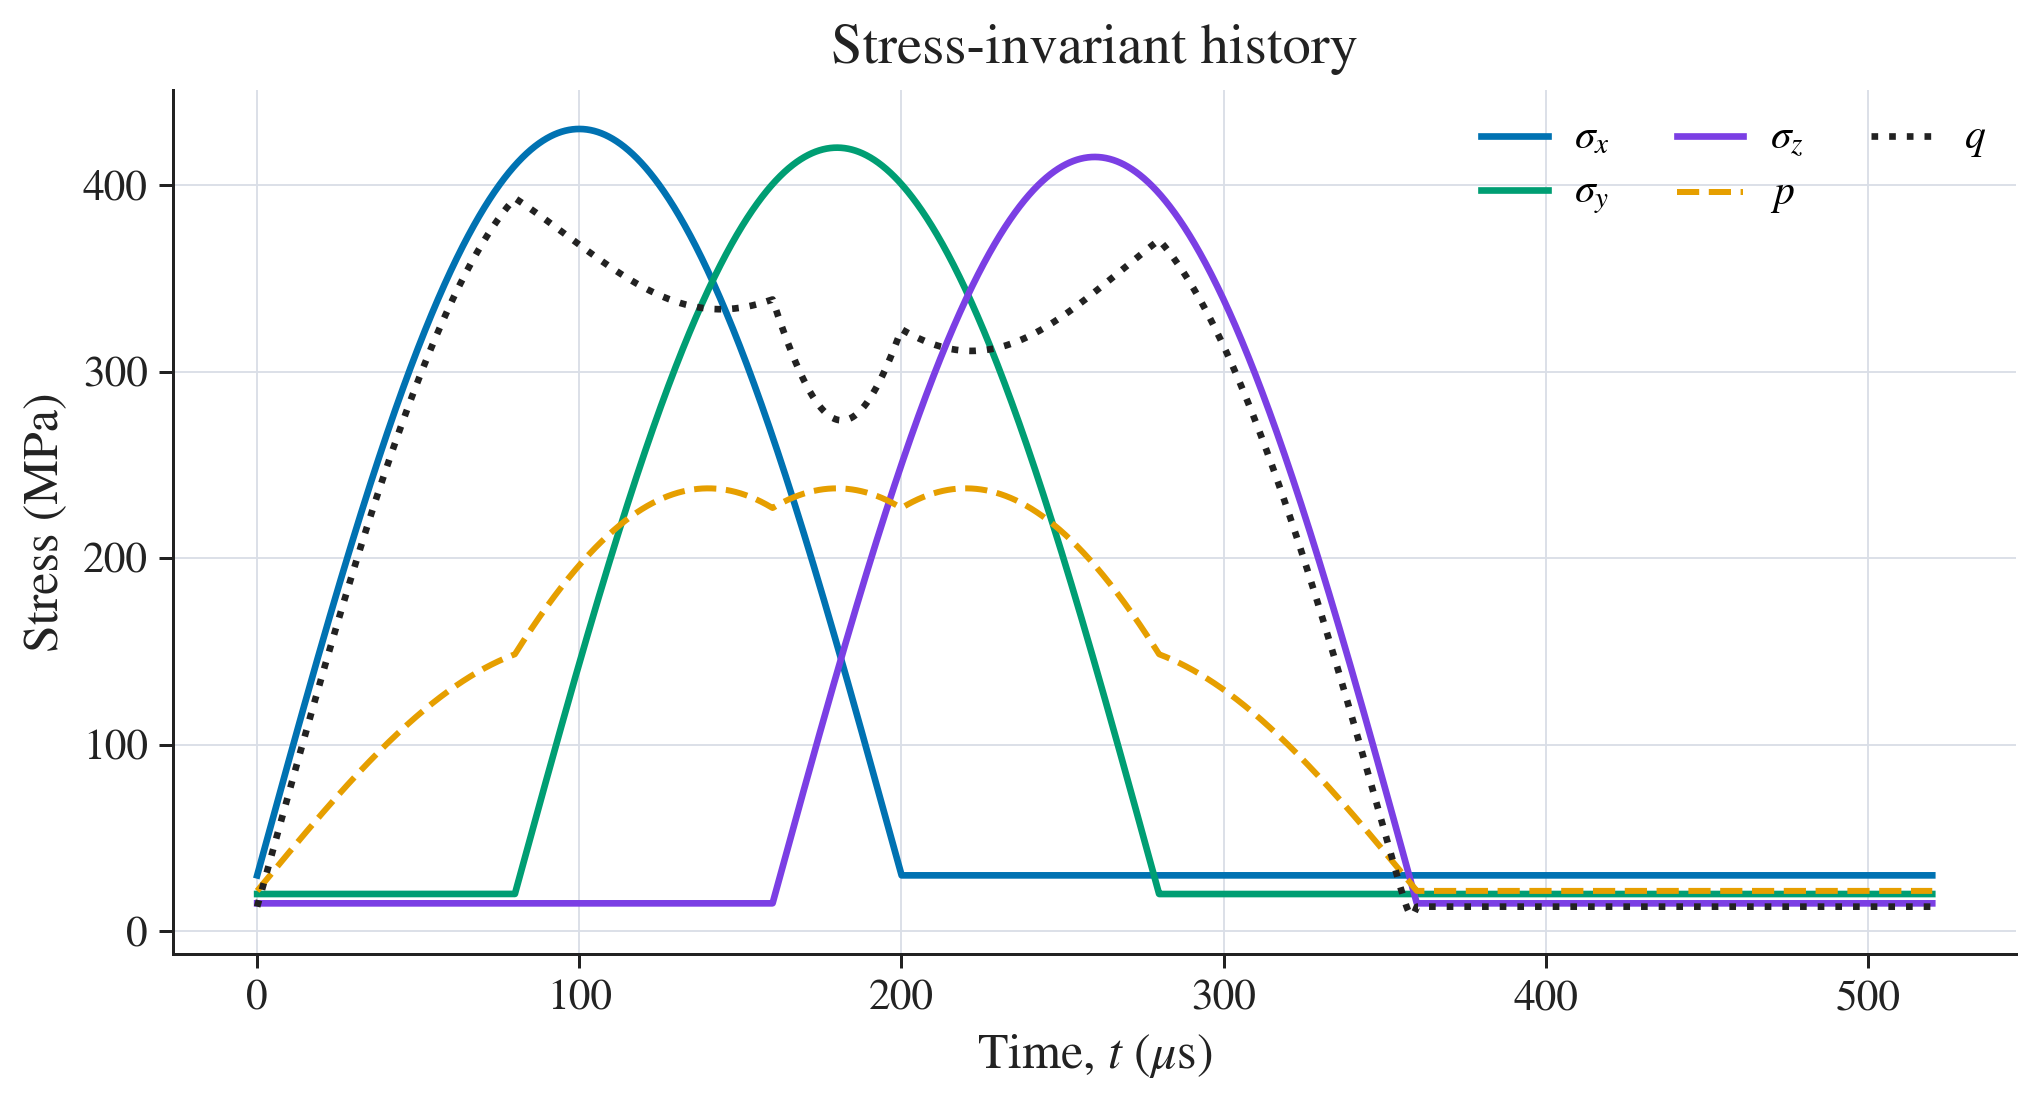
\includegraphics[width=0.92\linewidth]{figures/handbook_steps/step3_total_stresses_invariants.png}
  \caption{Step~3 default sandstone asynchronous XYZ case: total principal stresses and the derived pressure/deviatoric invariants used by the stress-path tab.}
  \label{fig:step3-total-stresses-invariants}
\end{figure}

\begin{figure}[htbp]
  \centering
  
\includegraphics[width=0.92\linewidth]{figures/handbook_steps/step3_pq_trajectory.png}
  \caption{Step~3 default sandstone asynchronous XYZ case: $p$--$q$ trajectory coloured by elapsed loading time.}
  \label{fig:step3-pq-trajectory}
\end{figure}

\begin{figure}[htbp]
  \centering
  
\includegraphics[width=0.92\linewidth]{figures/handbook_steps/step3_failure_surface_comparison.png}
  \caption{Step~3 default sandstone asynchronous XYZ case: comparison of $q$ with the pressure- and Lode-angle-dependent failure surface $q_f$.}
  \label{fig:step3-failure-surface-comparison}
\end{figure}

\begin{figure}[htbp]
  \centering
  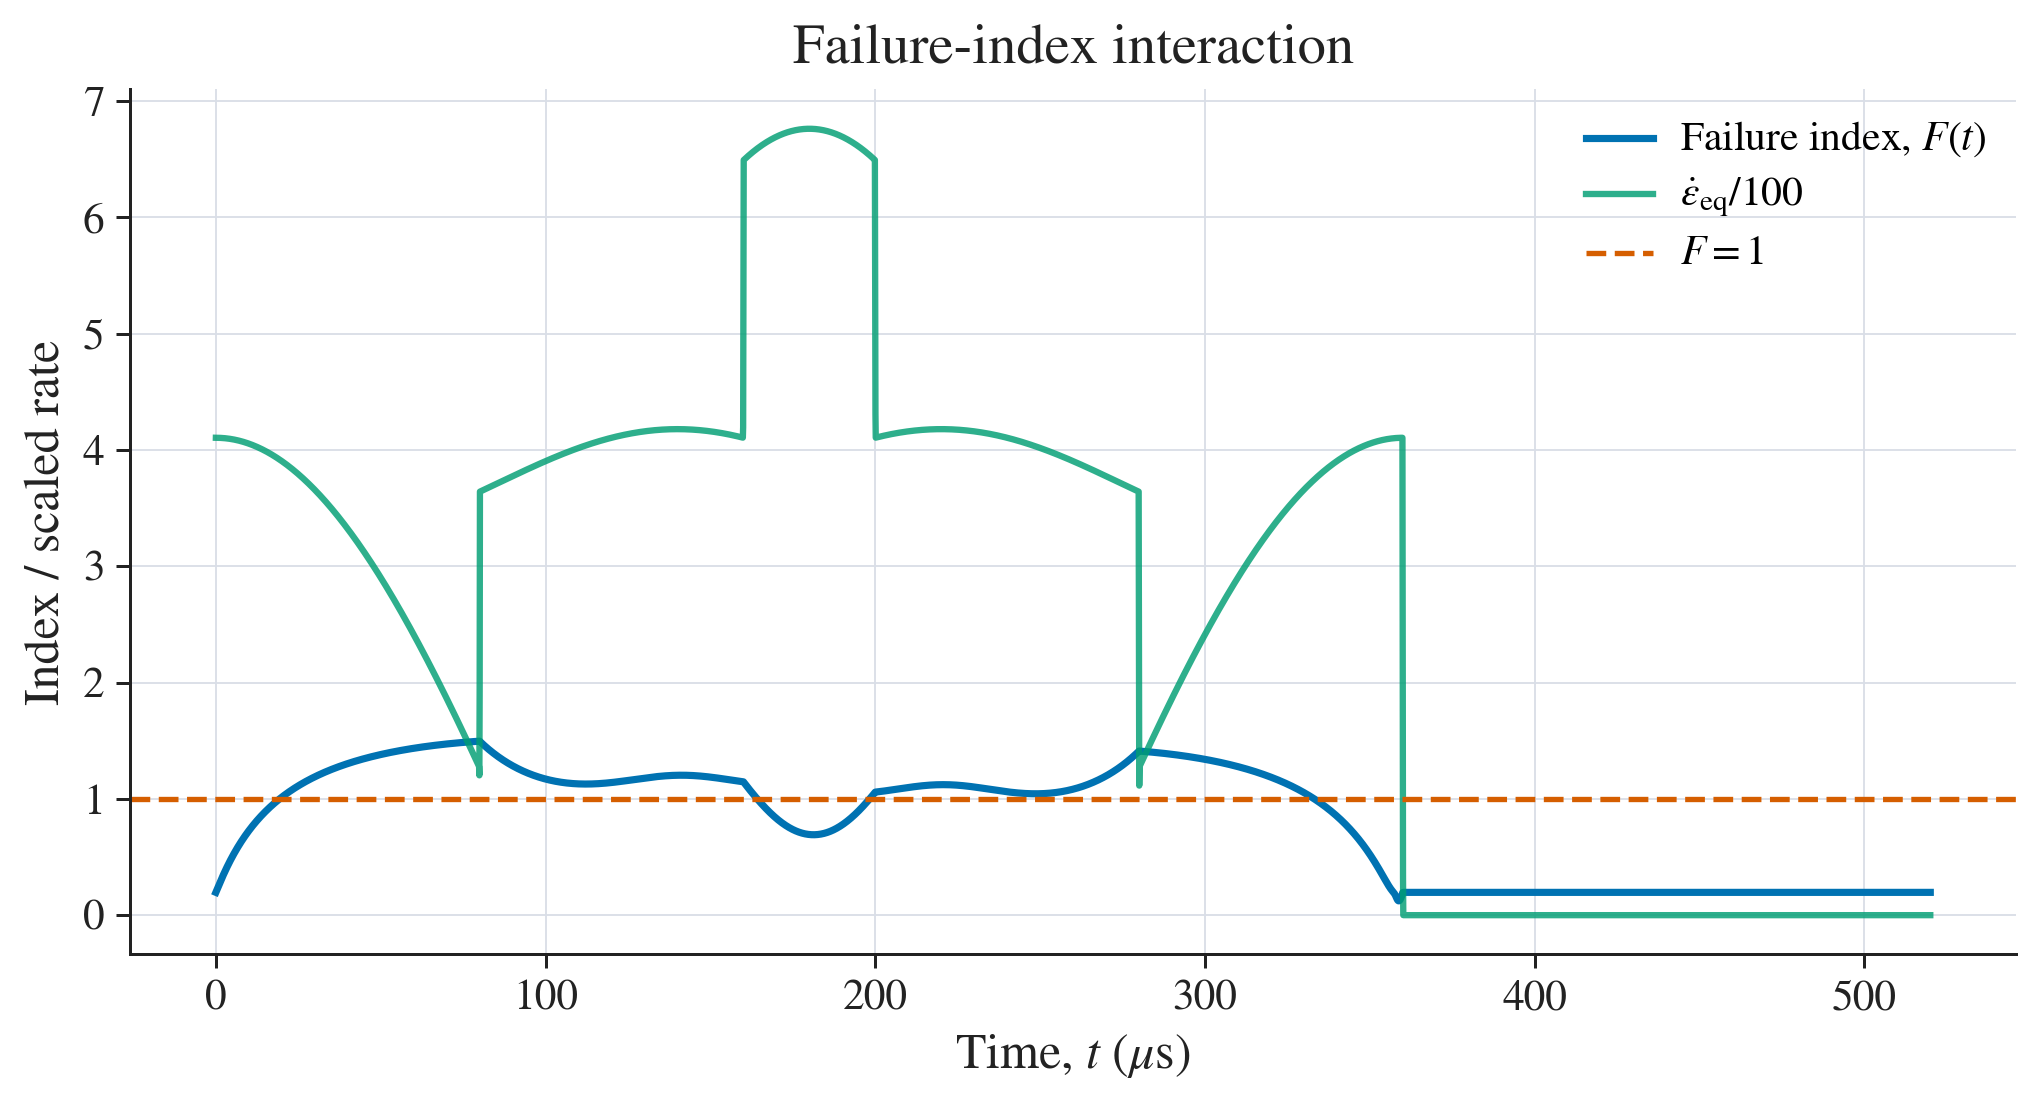
\includegraphics[width=0.92\linewidth]{figures/handbook_steps/step3_failure_index_strain_rate.png}
  \caption{Step~3 default sandstone asynchronous XYZ case: failure index $F=q/q_f$ and scaled equivalent deviatoric strain-rate indicator.}
  \label{fig:step3-failure-index-strain-rate}
\end{figure}

\section{Damage and energy equations (Step 4 tab)}\label{sec:damage}

\subsection{Damage evolution}

A Perzyna-type, saturating, rate-sensitive damage law is adopted
\cite{Perzyna1966,Murakami2012}. Damage is driven by the \emph{effective}
failure index, i.e.\ the stress carried by the intact material fraction,
\begin{equation}
  F_{\text{eff}}(t) \;=\; \bigl(1-D\bigr)\,F(t),
  \qquad F=q/q_f,
  \label{eq:Feff}
\end{equation}
so that the rate law reads
\begin{equation}
  \dot D \;=\; \frac{(1-D)^{\alpha}}{\tau_D}\,
              \left\langle\frac{F_{\text{eff}}-1}{F_0}\right\rangle^{m}
              \left(\frac{|\epsdot_{\text{eq}}|}{\epsdot_0}\right)^{\beta},
  \qquad D\in[0,1],
  \label{eq:damage-evol}
\end{equation}
where $\langle\cdot\rangle$ denotes the Macaulay bracket (damage grows
only when $F_{\text{eff}}>1$). The factor $(1-D)$ in \eqref{eq:Feff} is a
load-shedding feedback: as the material softens it carries less of the
applied deviatoric stress, so the effective overstress falls back toward
unity and the damage rate self-limits. The damage variable therefore rises
smoothly and saturates near $1-1/F_{\max}$, rather than jumping abruptly to
$D=1$ once the failure surface is first crossed. The exponents and time
scale are tabulated in Appendix~\ref{app:tables}.

\subsection{Stiffness and wave-speed degradation}
\begin{equation}
  E(D) \;=\; E_0\,(1-D),
  \qquad
  c_p(D) \;=\; c_{p0}\,\sqrt{\max(1-D,\,0)}.
\end{equation}

\begin{figure}[htbp]
  \centering
  
\includegraphics[width=0.92\linewidth]{figures/handbook_steps/step4_damage_trigger.png}
  \caption{Step~4 default sandstone asynchronous XYZ case: failure-index history and the threshold above which damage is allowed to grow.}
  \label{fig:step4-damage-trigger}
\end{figure}

\begin{figure}[htbp]
  \centering
  
\includegraphics[width=0.92\linewidth]{figures/handbook_steps/step4_cumulative_damage.png}
  \caption{Step~4 default sandstone asynchronous XYZ case: cumulative scalar damage and normalised damage-rate history.}
  \label{fig:step4-cumulative-damage}
\end{figure}

\begin{figure}[htbp]
  \centering
  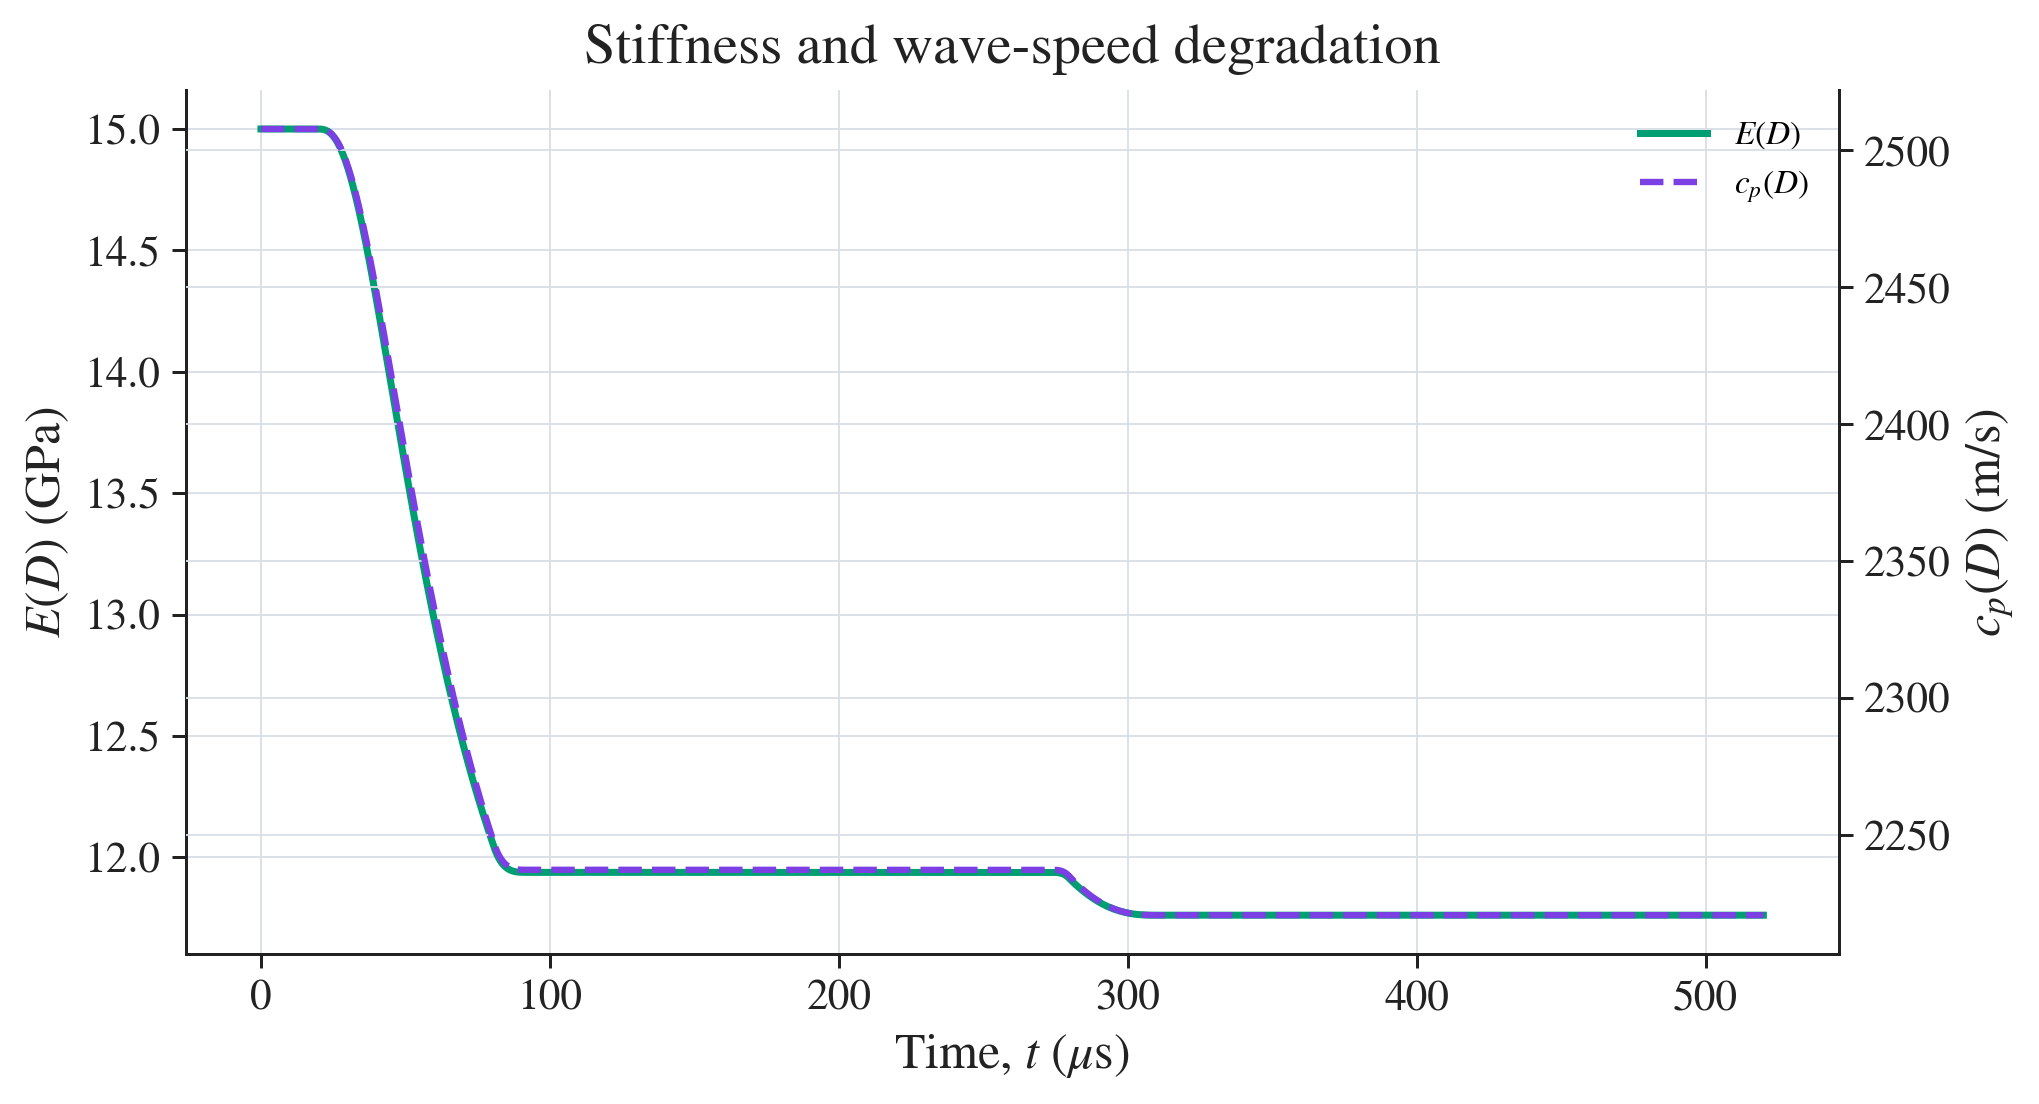
\includegraphics[width=0.92\linewidth]{figures/handbook_steps/step4_stiffness_wave_speed.png}
  \caption{Step~4 default sandstone asynchronous XYZ case: stiffness degradation and corresponding P-wave-speed reduction.}
  \label{fig:step4-stiffness-wave-speed}
\end{figure}

\begin{figure}[htbp]
  \centering
  
\includegraphics[width=0.92\linewidth]{figures/handbook_steps/step4_damage_profile.png}
  \caption{Step~4 default sandstone asynchronous XYZ case: synthetic specimen damage profile and central/symmetry descriptors used for DEM or experimental comparison.}
  \label{fig:step4-damage-profile}
\end{figure}

\subsection{Energy indicators per unit volume}
\begin{align}
  W_{\text{el}} &\;=\; \frac{1}{2E}\Bigl[\sig_x^{2}+\sig_y^{2}+\sig_z^{2}
                  -2\nu(\sig_x\sig_y+\sig_y\sig_z+\sig_z\sig_x)\Bigr], \\
  W_{\text{input}}(t) &\;=\; \int_{0}^{t}\!\bigl(\sig_x\epsdot_x+\sig_y\epsdot_y+\sig_z\epsdot_z\bigr)\,d\tau, \\
  W_{\text{diss}}(t) &\;=\; \int_{0}^{t} Y\,\dot D\,d\tau,
                  \qquad Y \;=\; W_{\text{el}}.
  \label{eq:Wdiss}
\end{align}
The dissipated energy \eqref{eq:Wdiss} is the continuum-damage-mechanics
form: $Y=W_{\text{el}}$ is the energy-release rate (the elastic energy
released as the modulus degrades), so $W_{\text{diss}}$ is non-negative,
remains zero until damage grows, and then increases monotonically. This is
preferred to the earlier elastic-cancellation estimate
$W_{\text{input}}-W_{\text{el}}$, which is near zero by construction for a
reversible elastic stress--strain field and therefore does not represent
the irreversible damage work. With stresses in MPa and dimensionless
strains, $W$ is in MJ\,m\textsuperscript{-3}.

\subsection{Synthetic DEM/experimental descriptors}

The damage profile $D(x)$ across the specimen is reconstructed from three
contributions (left wave, right wave, and central superposition), then
the following summary statistics are derived:
\begin{align}
  D_c &\;=\; \frac{\int_{\text{centre}}D(x)\,dx}{\int_{0}^{\Ls}D(x)\,dx}
         \quad (\text{central damage fraction}), \\
  S_x &\;=\; 1 - \frac{|D_{\text{left}}-D_{\text{right}}|}{D_{\text{left}}+D_{\text{right}}}
         \quad (\text{symmetry index}).
\end{align}
These are model indicators intended for planning and interpretation, not
substitutes for a real DEM simulation or CT scan; they should be
validated against measured fracture patterns whenever such data are
available.

\begin{figure}[htbp]
  \centering
  
\includegraphics[width=0.92\linewidth]{figures/handbook_steps/step4_energy_density_histories.png}
  \caption{Step~4 default sandstone asynchronous XYZ case: input, recoverable elastic, and dissipated energy-density histories. With the damage-coupled strain (\S\ref{sec:v6-energy}) the first law closes exactly, $W_{\mathrm{input}}=W_{\mathrm{el}}+W_{\mathrm{diss}}$: $W_{\mathrm{input}}$ ends above zero by exactly the dissipated part, $W_{\mathrm{el}}$ returns toward zero on unloading, and $W_{\mathrm{diss}}$ rises monotonically.}
  \label{fig:step4-energy-density-histories}
\end{figure}

\begin{figure}[htbp]
  \centering
  
\includegraphics[width=0.92\linewidth]{figures/handbook_steps/step4_power_density.png}
  \caption{Step~4 default sandstone asynchronous XYZ case: instantaneous mechanical power-density history.}
  \label{fig:step4-power-density}
\end{figure}

\begin{figure}[htbp]
  \centering
  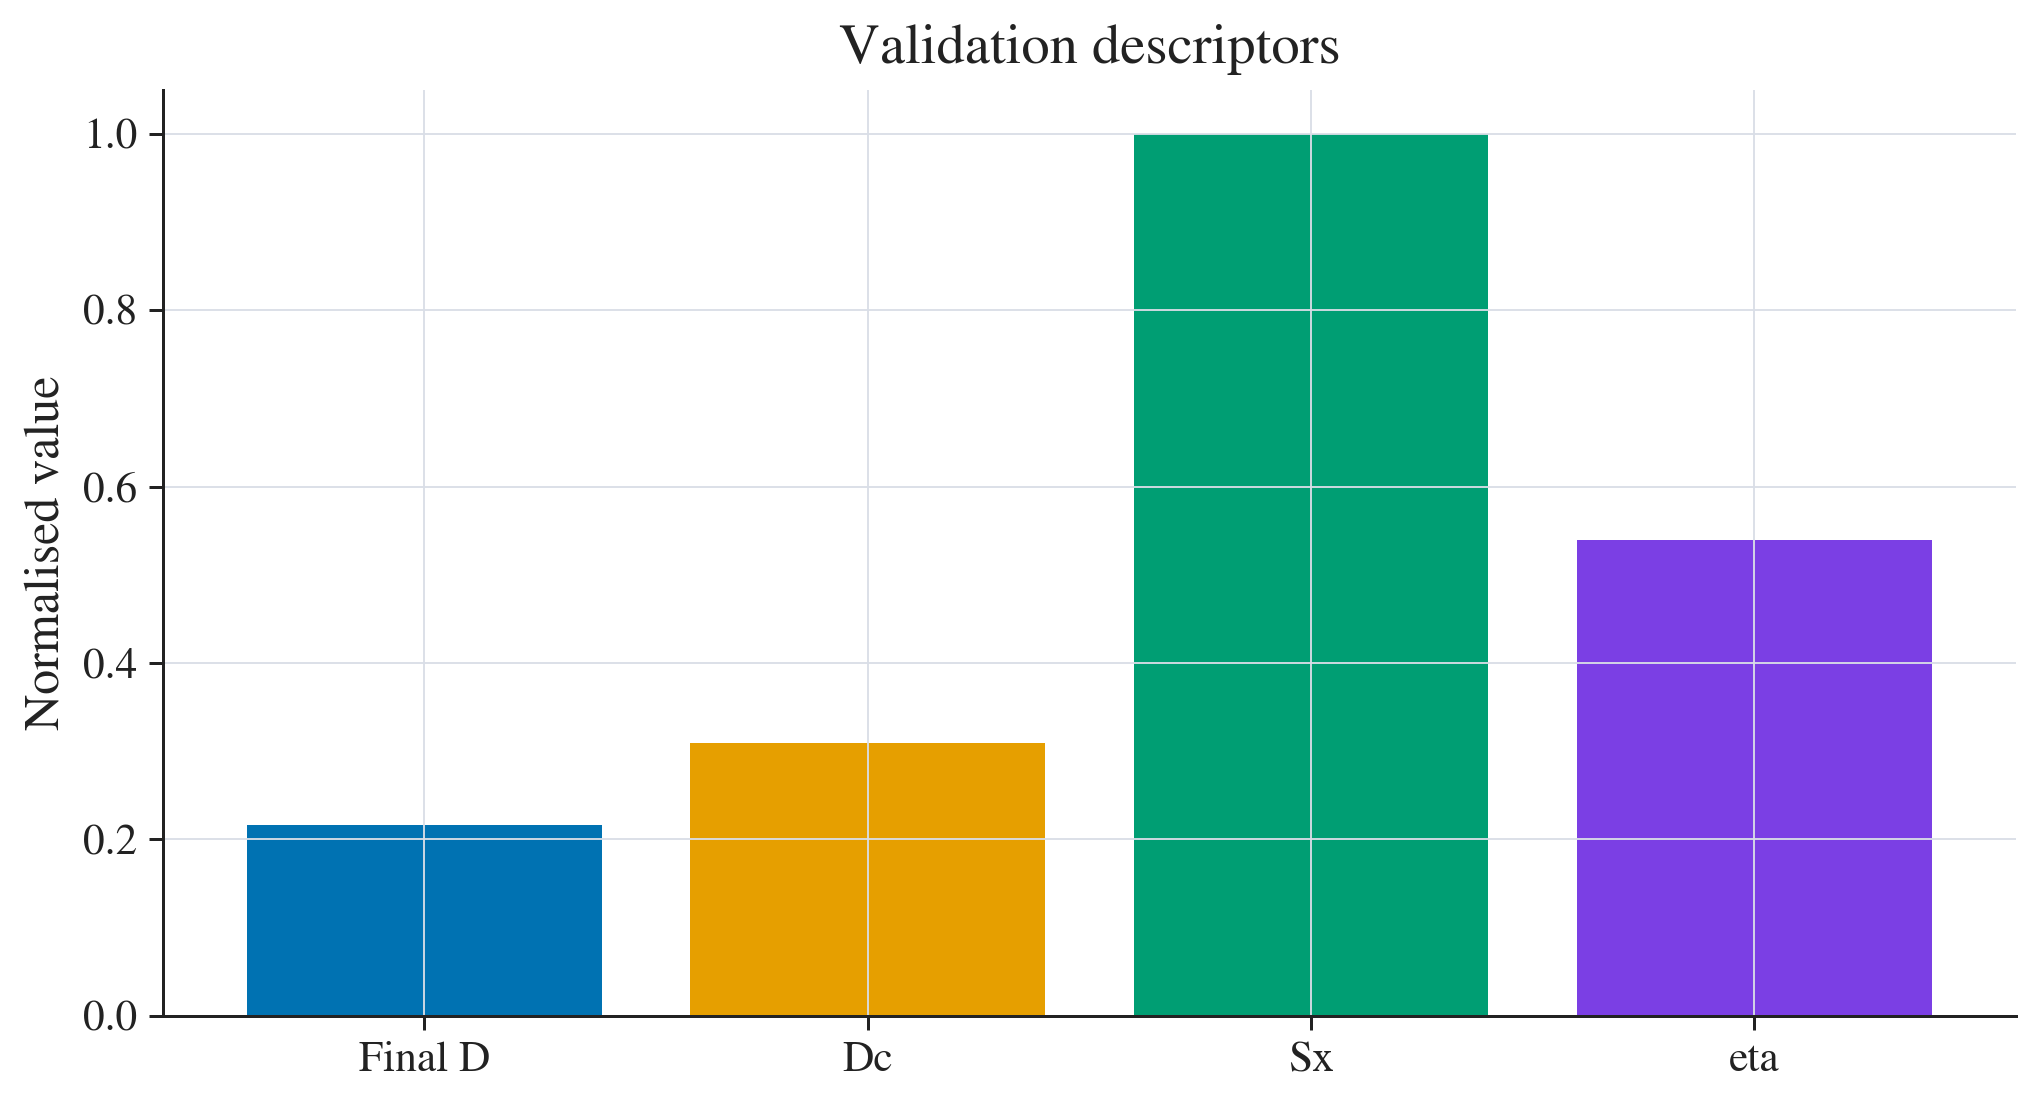
\includegraphics[width=0.92\linewidth]{figures/handbook_steps/step4_validation_descriptors.png}
  \caption{Step~4 default sandstone asynchronous XYZ case: scalar validation descriptors including final damage, central damage fraction, symmetry index, and superposition indicator.}
  \label{fig:step4-validation-descriptors}
\end{figure}

\begin{figure}[htbp]
  \centering
  
\includegraphics[width=0.92\linewidth]{figures/handbook_steps/step4_delay_sensitivity_indicators.png}
  \caption{Step~4 default sandstone asynchronous XYZ case: delay-sensitivity guide curves for final and central damage trends.}
  \label{fig:step4-delay-sensitivity-indicators}
\end{figure}

\section{Sidebar controls common to Steps~2--4}

\begin{description}[leftmargin=2em,style=nextline]
  \item[Control level] \emph{Guided} or \emph{Advanced}. Advanced exposes
    the failure parameters $A,B,n$, the Lode amplitude $a_\theta$, the
    damage time scale $\tau_D$, the saturation exponent $\alpha$, the
    overstress exponent $m$, the rate exponent $\beta$, the reference
    strain rate $\epsdot_0$, and the normalisation $F_0$.
  \item[Use Step 1 setup] When ticked (default if Step~1 has been run),
    the material, geometry, prestress, pulse amplitude, pulse duration,
    and loading dimensionality are read from the shared session state.
    Untick to enter a standalone setup.
  \item[Analysis goal] A workflow preset that opens the most relevant tab
    first and pre-fills sensible defaults (the calibration goals start in
    Advanced mode with the model constants exposed). In the stepped workflow
    it is set \emph{automatically} from the active step --- Step~2 $\to$
    \emph{Quick validation}, Step~3 $\to$ \emph{Stress-path focus}, Step~4
    $\to$ \emph{Damage calibration} --- so it is not re-selected on every
    step; the standalone (combined) view still shows the selector with all
    four goals. The governing equations are identical across goals.
\end{description}

\section{Export from Step~4}

A single CSV download bundles every time-series produced by the
wave/damage module: input pulses, $\sig_x,\sig_y,\sig_z$, the invariants
$p,q,\theta$, the failure surface $q_f$, the failure index $F$, the
equivalent strain rate, $D,\dot D,E(D),c_p(D),W_{\text{input}},
W_{\text{el}},W_{\text{diss}}$.

\section{Advanced constitutive options (Version~6)}\label{sec:v6-advanced}

Version~6 adds three physics upgrades, all exposed under \emph{Advanced} mode on
the Step~4 page. They are opt-in: the defaults reproduce the earlier scalar,
quasi-static behaviour except where noted, so existing results are unchanged.

\subsection{True-triaxial and rate-dependent failure envelope}\label{sec:v6-envelope}

The failure envelope keeps the form $q_f=(A_{\mathrm{eff}}+B_{\mathrm{eff}}\,
p^{n})\,h(\theta)$, but the deviatoric shape $h(\theta)$ and the rate dependence
are now selectable.

\paragraph{Deviatoric (Lode) shape.} Three forms are offered. The historical
``legacy'' cap $h=1+a_\theta(1-\cos 3\theta)$ \emph{raises} the extension
meridian above compression, which is the wrong sense for brittle rock. The new
default, an extension-weakened Lode interpolation, and the convex
Willam--Warnke form both use the extension/compression meridian ratio
$\rho_t/\rho_c$ and make extension correctly \emph{weaker} than compression
(Figure~\ref{fig:v6-lode}):
%
\begin{equation}
h_{\mathrm{Lode}}(\theta)=1-(1-\rho)\,\tfrac{1-\cos 3\theta}{2},\qquad
\rho=\rho_t/\rho_c\in(0.5,1],
\end{equation}
%
with $\theta=0$ the compression meridian and $\theta=60^\circ$ the extension
meridian. The intermediate principal stress ($\sigma_2$, true-triaxial) effect
therefore enters through the Lode angle with the physically correct sign;
$\rho_t/\rho_c=1$ recovers the $\sigma_2$-independent (von~Mises) circle. The
default is the Lode form with $\rho_t/\rho_c=0.70$.

\begin{figure}[htbp]
  \centering
  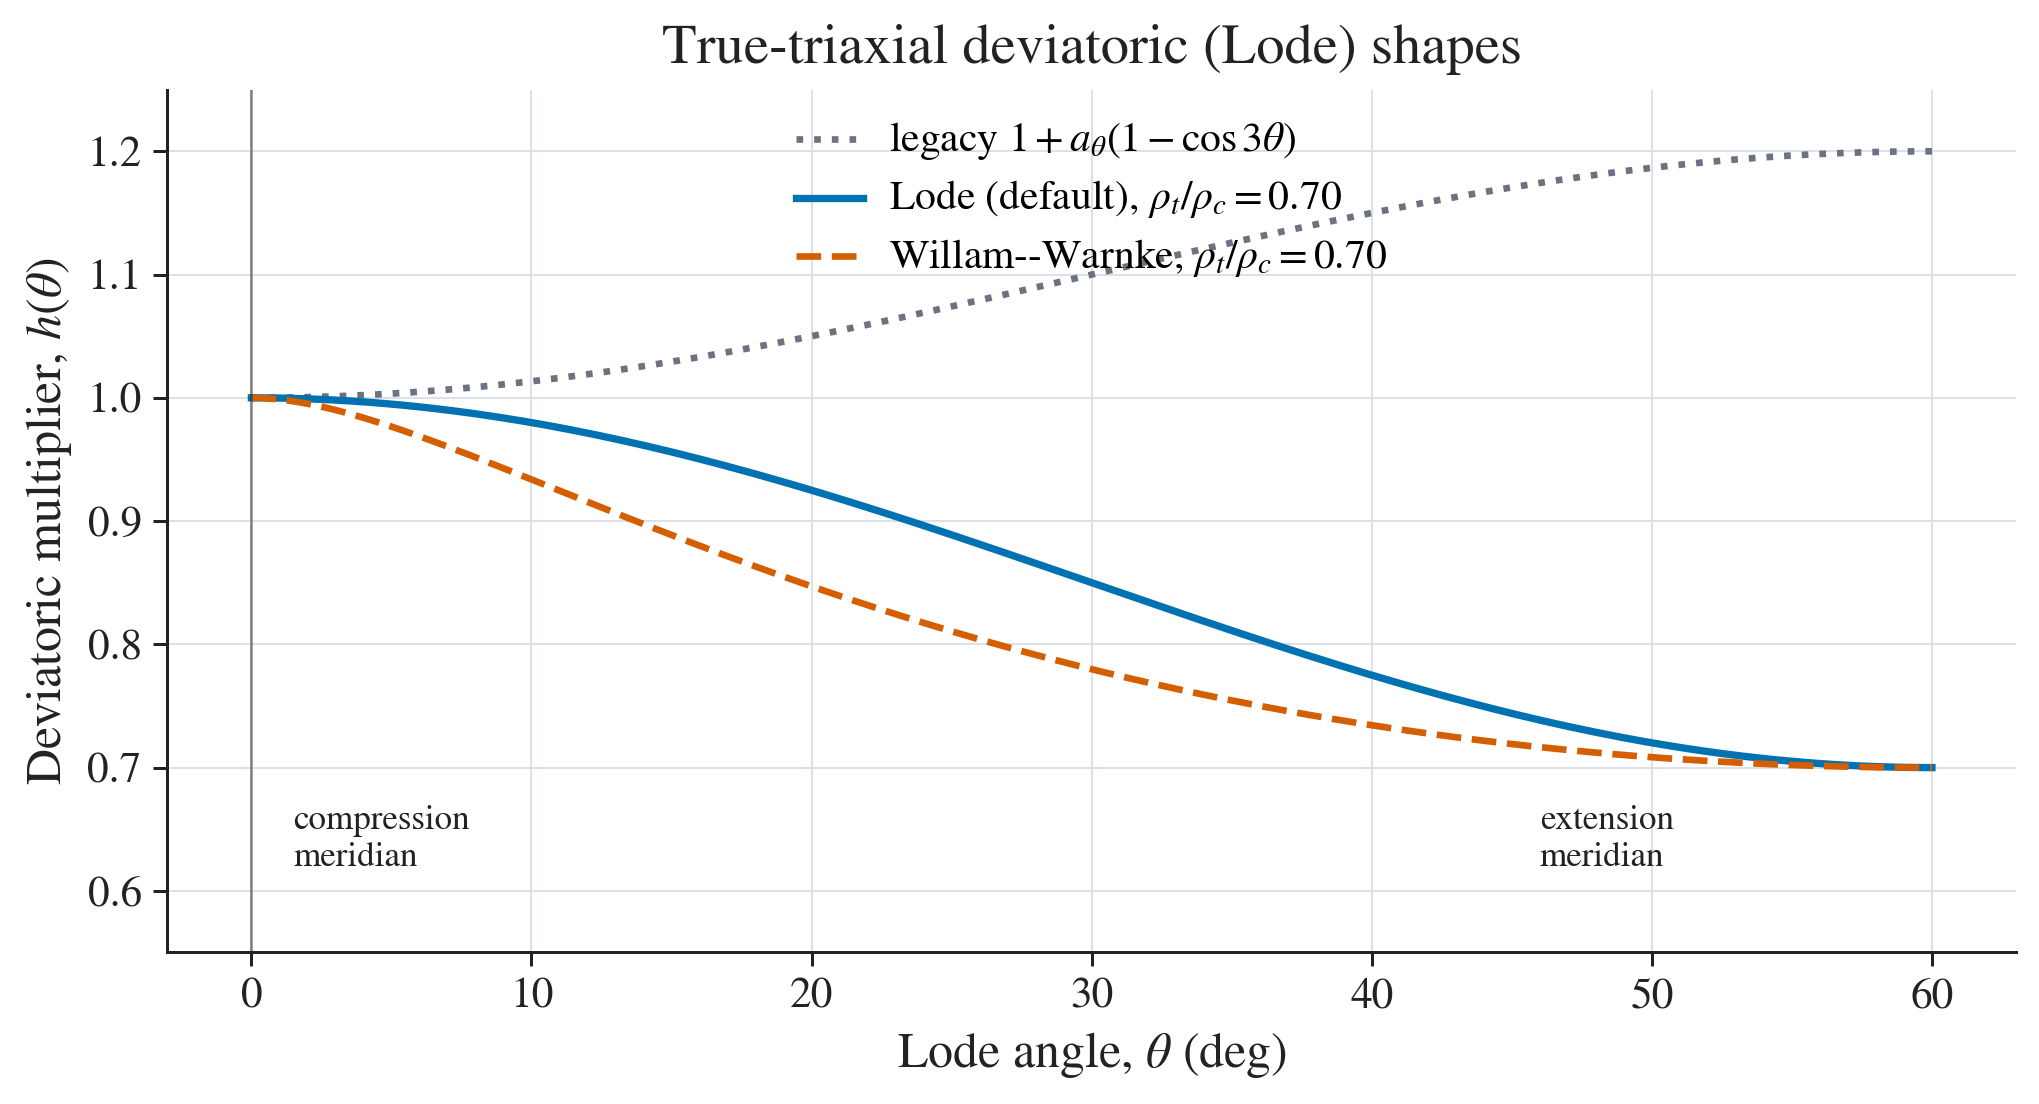
\includegraphics[width=0.82\linewidth]{figures/handbook_steps/step3_lode_shapes.png}
  \caption{Deviatoric (Lode) strength multiplier $h(\theta)$ for the three
  selectable envelopes. The legacy cap strengthens the extension meridian; the
  default Lode and the Willam--Warnke forms correctly weaken it
  ($\rho_t/\rho_c=0.70$ shown), capturing the intermediate principal stress
  effect.}
  \label{fig:v6-lode}
\end{figure}

\paragraph{Rate-dependent envelope.} Optionally, a dynamic increase factor
inflates the envelope so the failure \emph{onset} shifts with strain rate, in
addition to the rate term already in the damage law:
%
\begin{equation}
A_{\mathrm{eff}}=A\,\mathrm{DIF},\quad B_{\mathrm{eff}}=B\,(\mathrm{DIF}\text{ or }1),\qquad
\mathrm{DIF}=1+b_{\mathrm{env}}\log_{10}\!\max\!\Big(\frac{|\dot\varepsilon_{\mathrm{eq}}|}{\dot\varepsilon_0},1\Big).
\end{equation}
%
The slope $b_{\mathrm{env}}$ may act on the cohesion $A$ alone or on both $A$ and
$B$; the default is the quasi-static surface (no envelope DIF), with the rate
effect carried only by the damage kinetics. Figure~\ref{fig:v6-rate} shows the
envelope DIF over four decades of strain rate.

\begin{figure}[htbp]
  \centering
  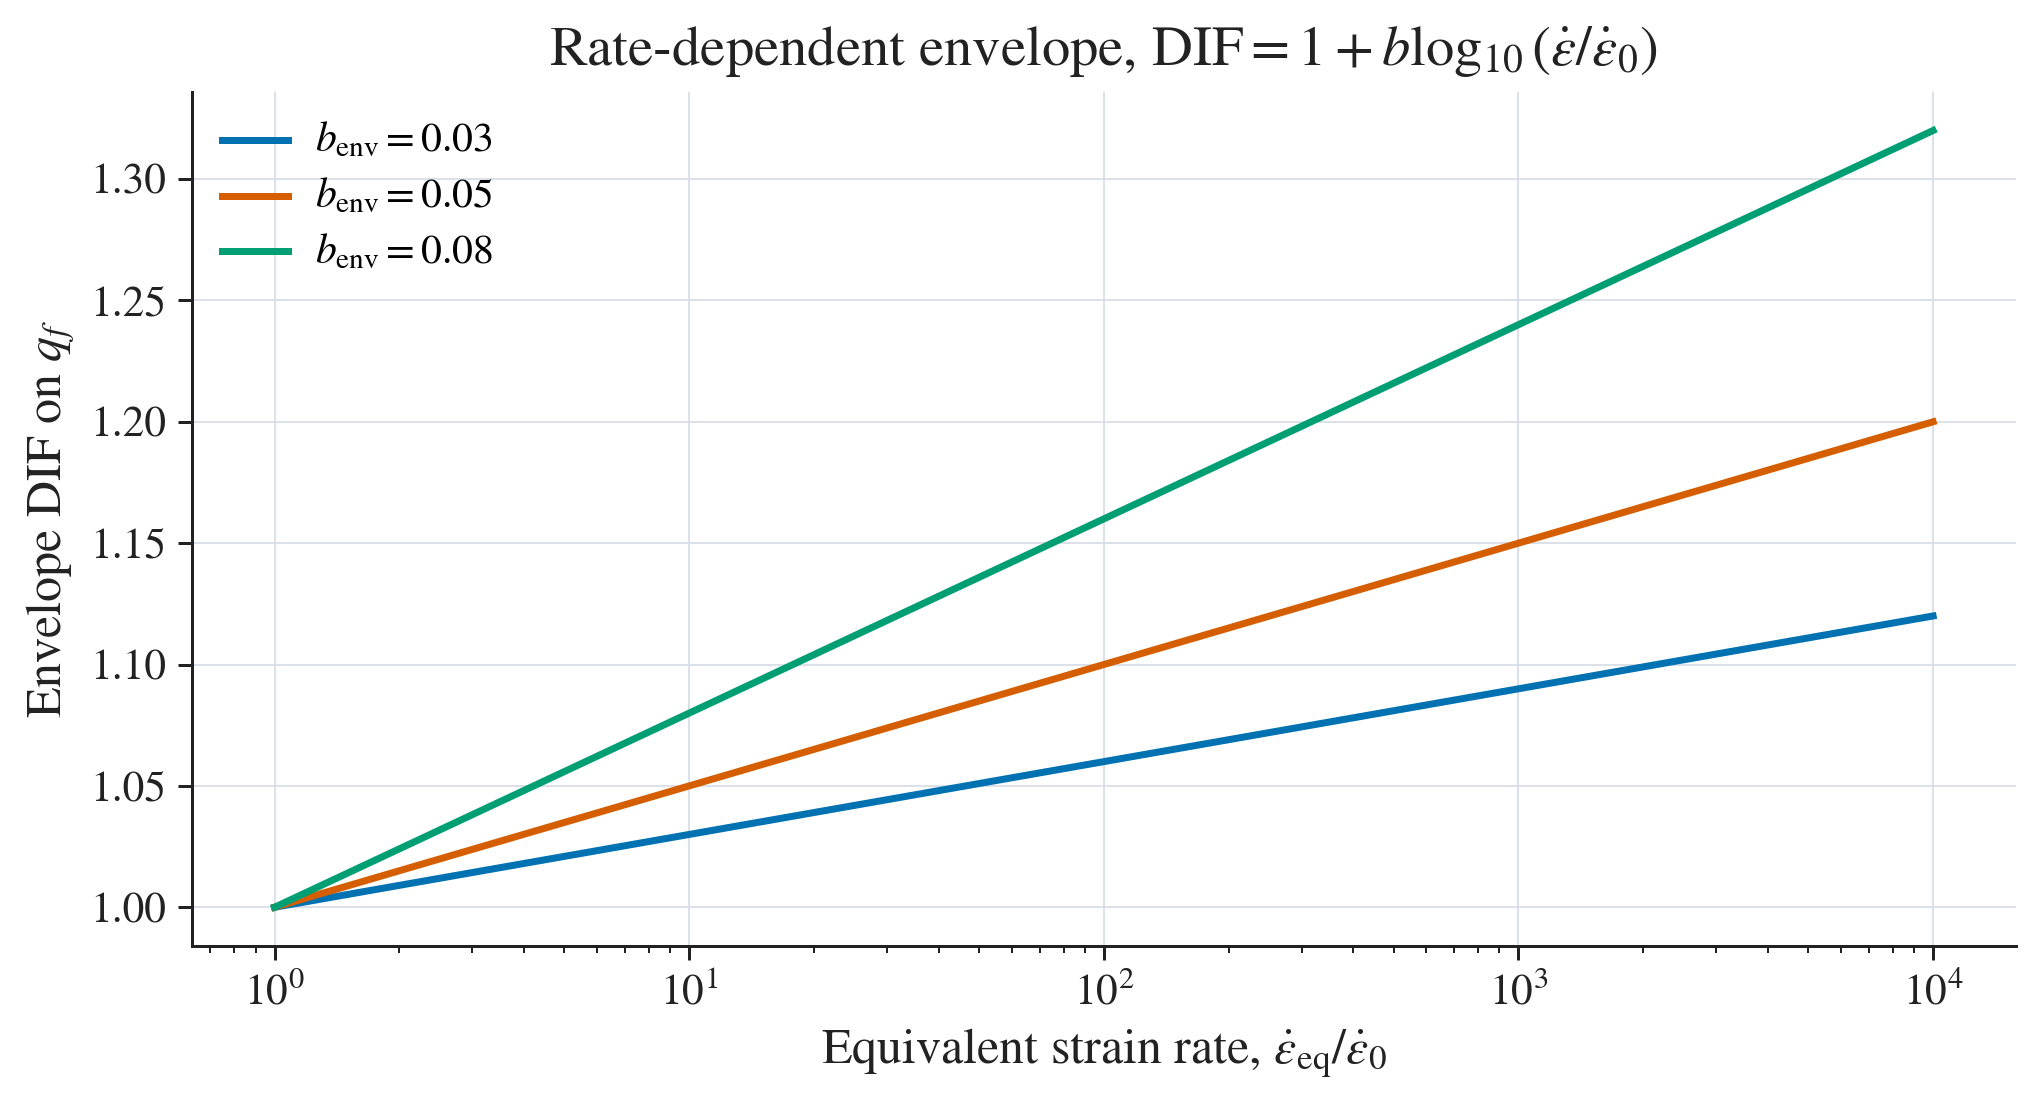
\includegraphics[width=0.82\linewidth]{figures/handbook_steps/step3_rate_dependent_envelope.png}
  \caption{Optional rate-dependent envelope: the dynamic increase factor applied
  to $q_f$ as a function of normalised equivalent strain rate, for three values
  of the slope $b_{\mathrm{env}}$.}
  \label{fig:v6-rate}
\end{figure}

\subsection{Energy-balance-consistent damage dissipation}\label{sec:v6-energy}

The damage dissipation is now derived from a single constitutive relation so the
first law closes by construction. Damage degrades the secant modulus to
$E_0(1-D)$, so the specimen carries the damage-coupled (effective-compliance)
elastic strain
%
\begin{equation}
\varepsilon_i=\frac{\sigma_i-\nu(\sigma_j+\sigma_k)}{E_0\,(1-D)},\qquad
W_{\mathrm{input}}=\int_0^t \sigma_i\,\dot\varepsilon_i\,d\tau,\qquad
W_{\mathrm{el}}=\tfrac12\,\sigma_i\varepsilon_i,
\end{equation}
%
and the dissipated energy is the part of the input work that cannot be returned
on unloading,
%
\begin{equation}
W_{\mathrm{diss}}=W_{\mathrm{input}}-W_{\mathrm{el}}=\int_0^t Y\,\dot D\,d\tau\;\ge 0,
\qquad\Longrightarrow\qquad W_{\mathrm{input}}=W_{\mathrm{el}}+W_{\mathrm{diss}}.
\end{equation}
%
This replaces the earlier mix of an undamaged-elastic input work and a separate
$\int Y\,dD$ sum, which did not balance. The corrected partition is the one
plotted in Figure~\ref{fig:step4-energy-density-histories}.

\subsection{Orthotropic (anisotropic) damage tensor}\label{sec:v6-orthotropic}

Blasting-induced fracturing is directional: cracks open perpendicular to the
local tension, so the stiffness and wave-speed loss differ by direction. Version~6
offers a diagonal damage tensor $D=\mathrm{diag}(D_x,D_y,D_z)$ aligned with the
bars (which are the principal loading directions in the rig). Each component is
driven by the directional tensile (extensile) strain through the same overstress
kinetics,
%
\begin{equation}
\dot D_i=\frac{(1-D_i)^{\alpha}}{\tau_D}
\Big\langle\frac{(1-D_i)F_i-1}{F_0}\Big\rangle^{m}
\Big(\frac{|\dot\varepsilon_{\mathrm{eq}}|}{\dot\varepsilon_0}\Big)^{\beta},
\qquad
F_i=\frac{\langle-\varepsilon_i\rangle_+}{\varepsilon_{t0}},\quad
\varepsilon_{t0}=\frac{\sigma_t}{E_0},
\end{equation}
%
for $i=x,y,z$. Damage grows only under directional extension ($\langle\cdot
\rangle_+$ is the positive part, so there is no damage in pure compression) ---
the tension-driven anisotropy of blasting. Axial X compression therefore drives
the lateral components $D_y,D_z$ (axial splitting) while $D_x\approx 0$, and
confinement on an axis suppresses its damage (Figure~\ref{fig:v6-orthotropic}).
The per-axis modulus and wave speed degrade independently,
$E_i=E_0(1-D_i)$, $c_{p,i}=c_{p0}\sqrt{1-D_i}$
(Figure~\ref{fig:v6-directional}) --- the directional quantities the Tri-HB's
three orthogonal bars measure post-test, from which each $D_i$ is calibrated
component-by-component. A uniaxial split-Hopkinson bar cannot do this.

\begin{figure}[htbp]
  \centering
  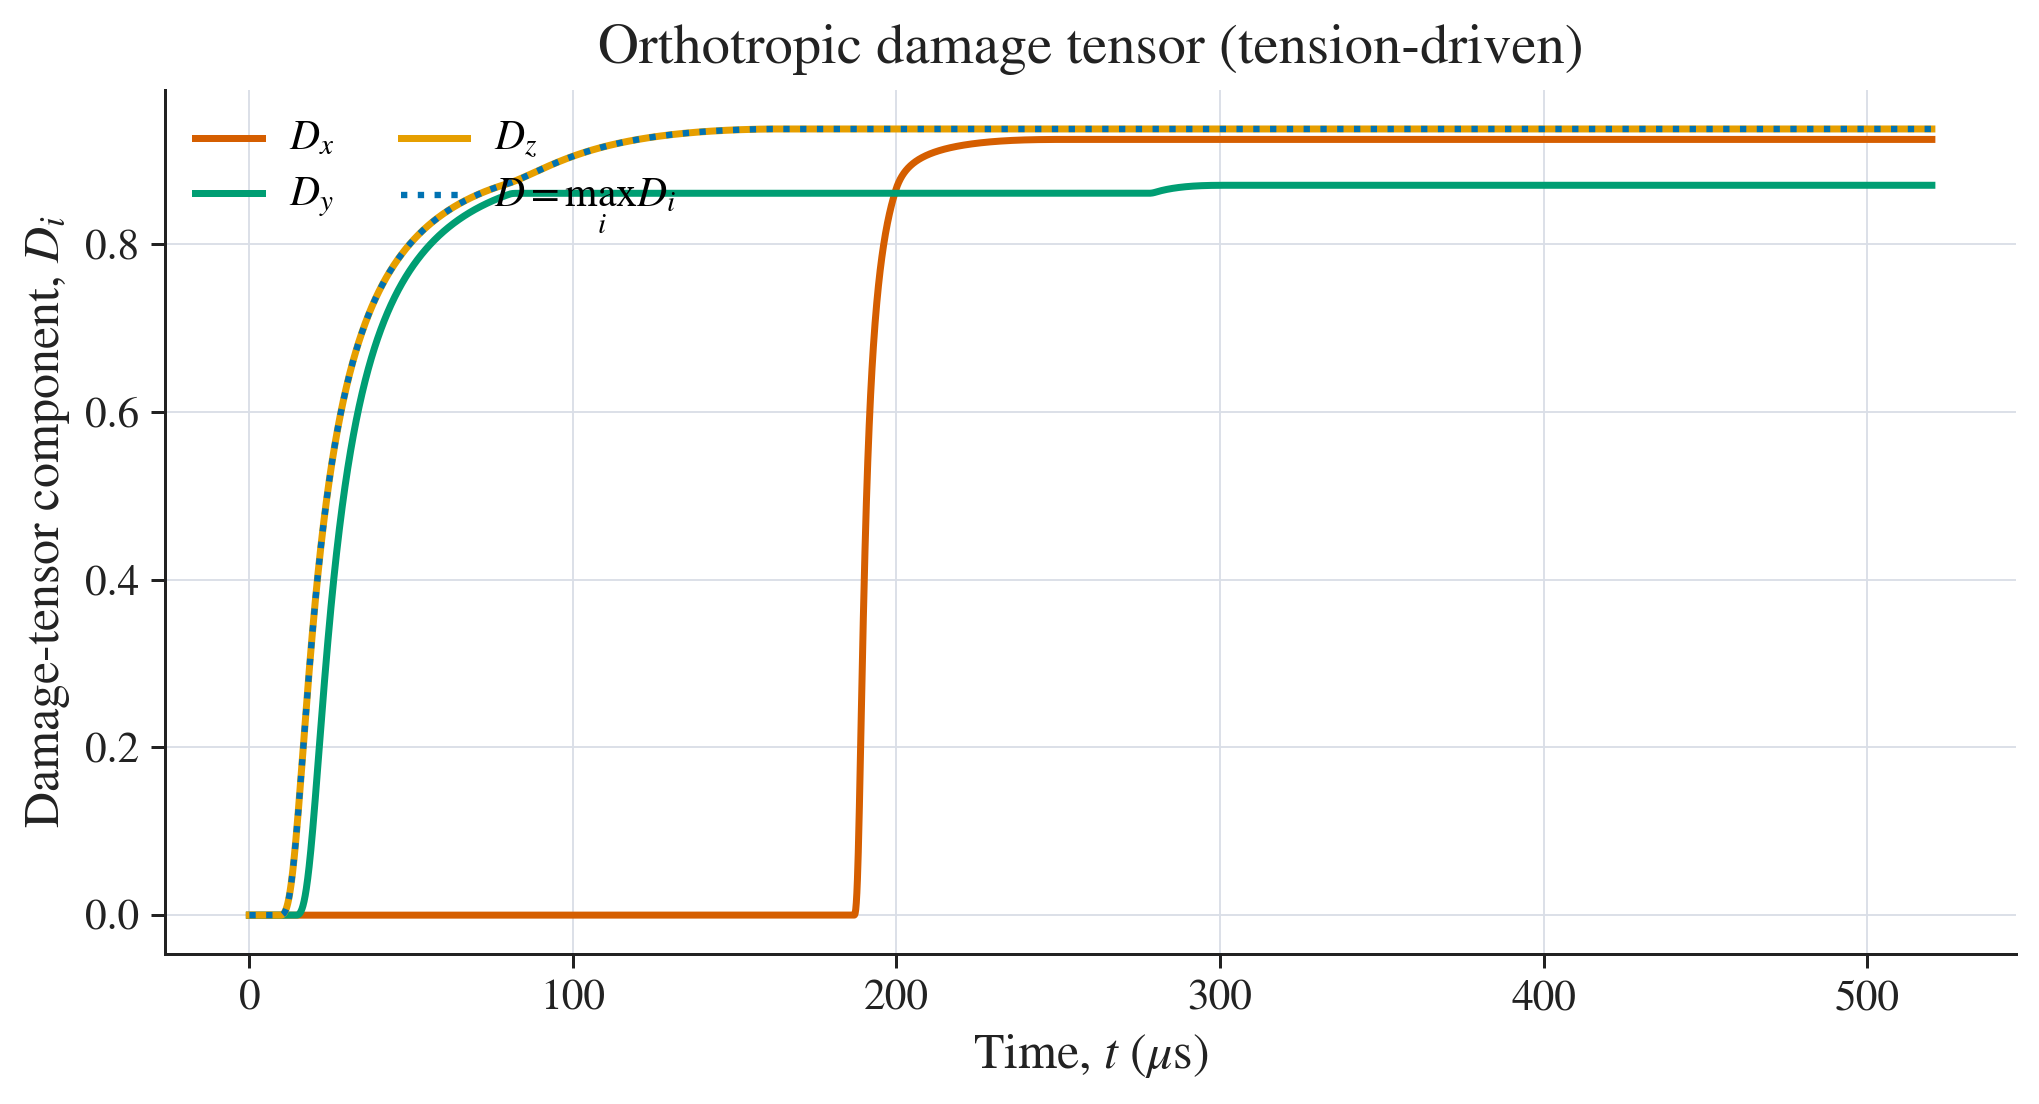
\includegraphics[width=0.82\linewidth]{figures/handbook_steps/step4_orthotropic_damage.png}
  \caption{Orthotropic (diagonal) damage-tensor components $D_x,D_y,D_z$ for the
  default sandstone asynchronous XYZ case. Each grows from its own directional
  extensile strain; the scalar $D=\max_i D_i$ governs the energy/stiffness
  summary.}
  \label{fig:v6-orthotropic}
\end{figure}

\begin{figure}[htbp]
  \centering
  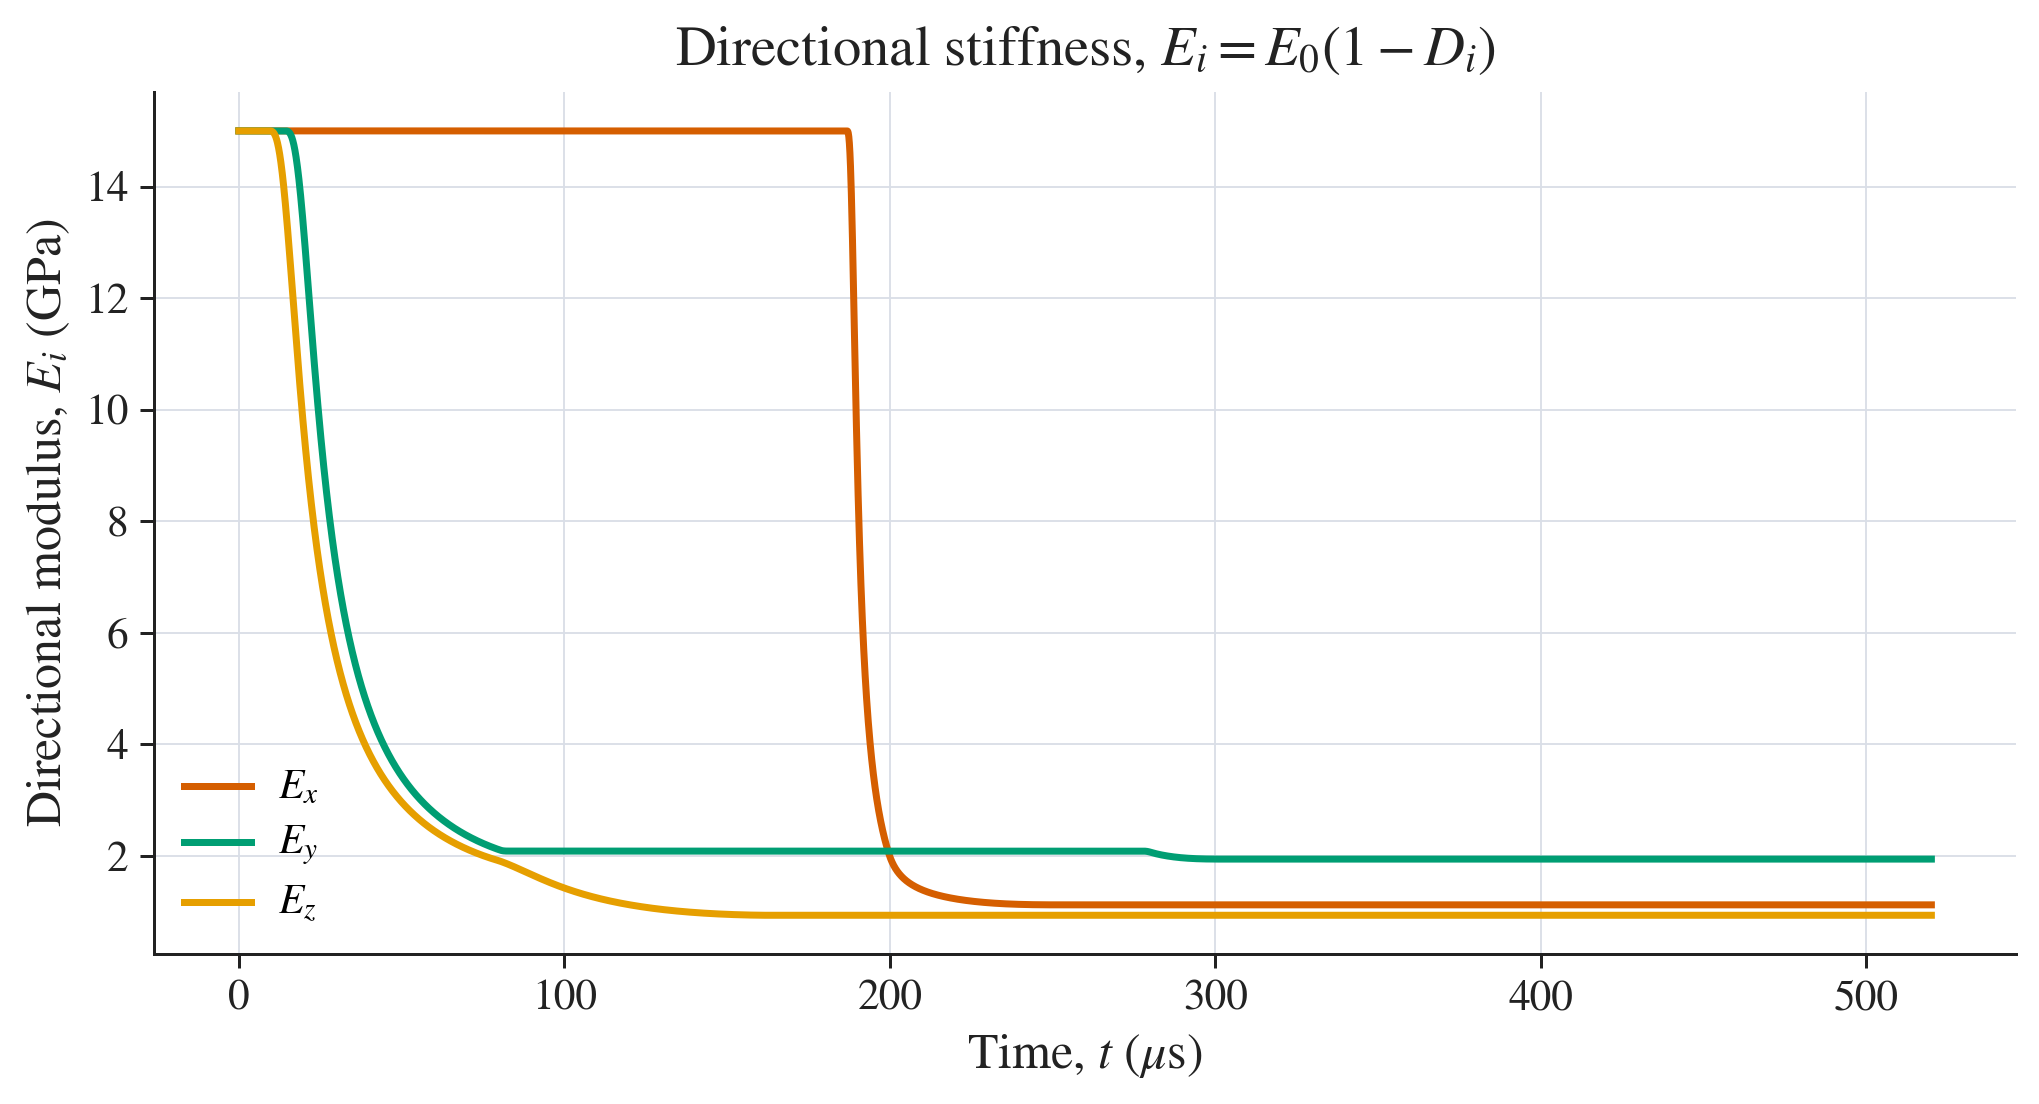
\includegraphics[width=0.82\linewidth]{figures/handbook_steps/step4_directional_stiffness.png}
  \caption{Directional stiffness degradation $E_i=E_0(1-D_i)$ for the orthotropic
  damage tensor --- the per-axis modulus loss measurable on each of the three
  bar pairs.}
  \label{fig:v6-directional}
\end{figure}

\begin{conceptbox}[Stage-1 scope]
The Version~6 orthotropic model is Stage~1: tension-driven directional damage
growth plus directional stiffness/wave-speed degradation. The energy partition
uses the scalar aggregate $D=\max_i D_i$ so the first law stays consistent for
any loading. A full anisotropic energy partition, unilateral crack-closure
stiffness recovery in compression, and a full second-order damage tensor with
principal-direction rotation are Stage~2--3; see
\texttt{docs/validation\_calibration\_plan.md}~\S11 for the roadmap and the
component-by-component calibration route.
\end{conceptbox}

\section{Document generation: Step~6}\label{sec:docgen}

The Step~6 page (\emph{Report and Presentation}) turns the current run into
ready-to-share documents through two tabs. Both reuse the metrics table and the
\SI{600}{dpi} figure set that the Step~5 summary captures in session state (each
figure is stored together with its caption, its short reading guide, and the
\LaTeX{} of its governing equations), so the generated documents match the
Step~5 view exactly.

\begin{description}[leftmargin=2em,style=nextline]
  \item[Presentation tab] Builds a Beamer slide deck in the Handbook
    lecture style. The deck contains an automatically generated title slide,
    an overview slide, a test-configuration slide, one key-results slide per
    workflow step, and one slide per captured figure. Each figure slide is a
    two-column layout: the figure on the left, and on the right a short
    bulleted description followed by the figure's governing equations. A
    closing scope slide states the planning-grade modelling assumptions. The
    deck is compiled with \texttt{xelatex} (it falls back to the default theme
    when the Metropolis theme is unavailable).
  \item[Report tab] Builds a short article-class report: an overview, a
    test-configuration table, a grouped key-results table, the captured
    figures (each with its caption, bulleted description, and governing
    equations), and a scope/validation note. It is compiled with
    \texttt{pdflatex}.
\end{description}

Each tab offers three downloads: the compiled PDF, the editable \texttt{.tex}
source, and a self-contained ZIP (the \texttt{.tex} plus all figure PNGs) for
offline compilation. The workspace locates the \LaTeX{} engine even when it is
not on the launching shell's \texttt{PATH} (it also searches standard MiKTeX
and TeX~Live install directories) and enables silent on-the-fly package
installation, so a first cold run does not stall. If no engine is found, the
\texttt{.tex} and ZIP are still produced and the page reports the reason.


%==============================================================================
%  APPENDICES
%==============================================================================
\appendix

%==============================================================================
\chapter{Reference tables}\label{app:tables}
%==============================================================================

\section{Bar properties (42CrMo steel) -- default values}

These are the digital twin's default bar parameters; each is editable in
the Step~1 \emph{Experimental setup} sidebar tab.

\begin{center}
\begin{tabular}{@{}lcc@{}}
\toprule
\textbf{Quantity} & \textbf{Symbol} & \textbf{Default value} \\
\midrule
Young's modulus & $E_b$ & \SI{210}{GPa} \\
Density & $\rho_b$ & \SI{7850}{kg/m^{3}} \\
Bar wave speed & $\Cz$ & \SI{5172}{m/s} \\
Proportional limit & $\sigprop$ & \SI{1000}{MPa} \\
Yield stress (approx.) & $\sig_Y$ & \SI{1080}{MPa} \\
Acoustic impedance & $Z_b=\rho_b\Cz$ & \SI{40.6e6}{kg\,m^{-2}\,s^{-1}} \\
Round bar area (editable default $\Phi 50$) & $\Ab$ & \SI{1963}{mm^{2}} \\
Square bar area (\SI{50}{mm}$\times$\SI{50}{mm}) & $\Ab$ & \SI{2500}{mm^{2}} \\
\bottomrule
\end{tabular}
\end{center}

\section{Default specimen parameters in the simulator}
\begin{center}
\renewcommand{\arraystretch}{1.3}
\begin{tabular}{@{}lccccccc@{}}
\toprule
\textbf{Material} & $E_s$ (GPa) & $\sig_{c0}$ (MPa) & $\nu$ & $b_{\text{rate}}$ & $\epsdot_{\text{ref}}$ (s$^{-1}$) & $k_{\text{conf}}$ & $\eps_{\text{peak}}$ \\
\midrule
Sandstone & 15 & 80  & 0.20 & 0.18 & \num{1e-5} & 4.5 & 0.008 \\
Granite   & 50 & 180 & 0.25 & 0.12 & \num{1e-5} & 5.5 & 0.005 \\
Concrete  & 30 & 40  & 0.20 & 0.22 & \num{1e-5} & 4.0 & 0.006 \\
\bottomrule
\end{tabular}
\end{center}

Selecting a preset in the Step~1 sidebar populates the editable
$E_s$, $\sig_{c0}$, and $\nu$ fields from this table. The remaining
columns are hidden preset constants used by the Streamlit constitutive
model.

\section{Default damage-model parameters (Step 4 Advanced mode)}
\begin{center}
\renewcommand{\arraystretch}{1.3}
\begin{tabular}{@{}lcc@{}}
\toprule
\textbf{Symbol} & \textbf{Meaning} & \textbf{Default} \\
\midrule
$A$ & Failure-surface intercept & $3\,\text{UCS}_{\text{eff}}/(k_{\text{conf}}+2)$ \\
$B$ & Failure-surface pressure coefficient & $3(k_{\text{conf}}-1)/(k_{\text{conf}}+2)$ \\
$n$ & Failure-surface pressure exponent & 1 \\
$a_\theta$ & Lode-angle amplitude & 0.10 \\
$\tau_D$ & Damage time scale & \SI{30}{\micro s} \\
$\alpha$ & Saturation exponent & 1.0 \\
$m$ & Overstress exponent & 2.0 \\
$\beta$ & Rate exponent & 0.15 \\
$\epsdot_0$ & Reference strain rate & \SI{1.0}{s^{-1}} \\
$F_0$ & Failure-index normalisation & 1.0 \\
\bottomrule
\end{tabular}
\end{center}

\section{Useful identities}
\begin{align*}
  \text{Acoustic impedance:}\quad & Z=\rho\,c \\
  \text{Pulse transmission (Fresnel):}\quad
    & \frac{F_T}{F_I}=\frac{2Z_2}{Z_1+Z_2},
      \quad \frac{F_R}{F_I}=\frac{Z_2-Z_1}{Z_1+Z_2} \\
  \text{Dynamic Increase Factor:}\quad
    & \text{DIF}=1+b_{\text{rate}}\log_{10}
      \!\left[\max(\epsdot,\epsdot_{\text{ref}})/\epsdot_{\text{ref}}\right] \\
  \text{Mean pressure:}\quad & p=\tfrac{1}{3}(\sig_1+\sig_2+\sig_3) \\
  \text{Deviatoric stress:}\quad
    & q=\sqrt{\tfrac{1}{2}\bigl[(\sig_1-\sig_2)^{2}+(\sig_2-\sig_3)^{2}+(\sig_3-\sig_1)^{2}\bigr]} \\
  \text{Lode angle:}\quad
    & \cos(3\theta)=\tfrac{3\sqrt{3}}{2}J_3/J_2^{3/2} \\
  \text{P-wave modulus:}\quad
    & M=E(1-\nu)/[(1+\nu)(1-2\nu)] \\
  \text{Shear, bulk modulus:}\quad
    & G=E/[2(1+\nu)],\quad K=E/[3(1-2\nu)]
\end{align*}

%==============================================================================
\chapter{Suggested exercises}\label{app:exercises}
%==============================================================================

\begin{enumerate}[leftmargin=*,itemsep=4pt]
  \item In Mode~1 (gas-gun), determine the maximum striker velocity for
        which a granite specimen with \SI{50}{MPa} confinement remains
        within the bar proportional limit. Verify the hand calculation
        against the warning system of the digital twin.
  \item In Mode~3 (gas-gun coupled triaxial), test sandstone
        ($\sig_{c0}=\SI{80}{MPa}$, $k_{\text{conf}}=4.5$,
        $b_{\text{rate}}=0.18$) at striker velocity $V=\SI{20}{m/s}$ and
        three confining pre-stress levels: $\sig_2=\sig_3=0$,
        \SI{20}{MPa}, and \SI{40}{MPa}. Plot the predicted dynamic peak
        strength from \eqref{eq:mode3-peak} against confinement, and check
        whether the bar stress stays within $\sigprop$ in each case.
        Discuss why confinement strengthens the rock dynamically without
        increasing the bar stress.
  \item In Mode~4, keep $\sigpeak=\SI{400}{MPa}$ fixed and vary $\tau$ from
        \SI{50}{\micro s} to \SI{300}{\micro s}. Plot peak specimen stress
        against strain rate. Extract the rate-hardening parameter
        $b_{\text{rate}}$ and compare with the nominal value in
        Appendix~\ref{app:tables}.
  \item In Mode~5, run sandstone at $\sig_{\text{conf}}=\SI{30}{MPa}$ with
        $\Delta t_y=\Delta t_z=0$ (synchronous), then with
        $\Delta t_y=\SI{100}{\micro s}$, $\Delta t_z=\SI{200}{\micro s}$.
        Compare peak $\sig_x$, then open Step~2 and record
        $\Delta t^{\ast}$ and the regime classifier output. Discuss the
        link between $\Delta t^{\ast}$ and the change in peak strength.
  \item In Mode~6 (symmetric XYZ), find the peak specimen pressure
        achievable with single-pulse $\sigpeak=\SI{900}{MPa}$ (right at
        the bar limit). Compare with the maximum pressure achievable in
        Mode~4 before bar yielding.
  \item Derive equations \eqref{eq:sig-sym} and \eqref{eq:epsdot-sym}
        from first principles (force and velocity continuity), without
        consulting Chapter~\ref{ch:mode6}.
  \item Extend the symmetric-mode derivation to the case where the two
        opposing pulses have different amplitudes, say $\sigpeak^{+}$ and
        $\sigpeak^{-}$. Show that the specimen experiences both a squeeze
        proportional to $\sigpeak^{+}+\sigpeak^{-}$ and a net acceleration
        proportional to $\sigpeak^{+}-\sigpeak^{-}$. At what amplitude
        ratio does this degenerate into Mode~4 (one-sided) behaviour?
  \item In Mode~4, test sandstone with $\sigpeak=\SI{300}{MPa}$,
        $\tau=\SI{200}{\micro s}$, $\sig_2=\sig_3=\SI{30}{MPa}$. Run the
        simulation three times with $\sig_1=0$, $\SI{25}{MPa}$, and
        $\SI{50}{MPa}$. Export the $\sig$--$\eps$ CSV from each run,
        overlay the three curves, and verify that increasing $\sig_1$
        shifts the entire curve upward by a constant offset without
        changing peak strength. Explain why $\sig_1$ behaves differently
        from $\sig_2$ and $\sig_3$.
  \item In Step~1, run any Mode~4 case. Switch the inner radio to
        ``Experimental data analysis'' and choose \emph{Data source =
        Latest simulator result}. Confirm that the three-wave reduction
        reproduces the simulator's stress--strain curve. Switch to
        \emph{Transmitted-wave only} and verify that the two reductions
        agree once stress equilibrium is reached.
  \item Take the same Mode~4 simulator result and download the All
        Signals CSV. Re-upload it through the ``Upload bar strain
        gauges'' branch with column mapping. Verify the reduced curve
        matches the simulator-derived curve, then deliberately mis-set
        the strain unit (e.g.\ claim ``microstrain'' for data stored as
        strain) and observe how the energy sanity warning fires.
  \item Move to Step~3 with any asynchronous Mode~5 simulator result.
        Read $\Delta t^{\ast}$ and the regime classifier off the Wave
        model tab, then trace the $p$--$q$ path in the Stress path tab.
        Identify the instant at which $F(t)=q(t)/q_f(t)$ first exceeds
        unity and compare with the time at which damage starts to grow
        on the Damage evolution tab in Step~4.
  \item Choose any test case of interest and download all four file
        types (Signals CSV, $\sig$--$\eps$ CSV, Configuration JSON, Full
        XLSX). Open the JSON file in a text editor and identify:
        (a) the simulator version, (b) the export timestamp, (c) the bar
        plasticity warning state, (d) the peak specimen stress. Discuss
        how this metadata supports reproducibility in a research
        context.
\end{enumerate}

%==============================================================================
%  BACK MATTER
%==============================================================================
\backmatter

\printbibliography[heading=bibintoc,title={References}]

\end{document}
